\documentclass[12pt]{article}

\usepackage[T1]{fontenc}
\usepackage{mathptmx}
\usepackage{amsmath}
\usepackage{amssymb}
\usepackage{graphicx}
\usepackage[title, titletoc]{appendix}
\usepackage{url}
%\usepackage[activeacute,spanish_PI]{babel}
\usepackage{fancyhdr}
\usepackage{color}
%\usepackage{newverbs}
%\usepackage{spverbatim}
\usepackage{tipa}
\usepackage{soul}
%\usepackage{listings}
\usepackage{enumitem}
\usepackage[colorlinks, linkcolor=link, citecolor=link, filecolor=link,pagecolor=link, urlcolor=link]{hyperref}
\usepackage{longtable}
\usepackage{caption}
\usepackage{fancyvrb}
\usepackage{rotating}

\setcounter{topnumber}{3}
\setcounter{bottomnumber}{2}
\setcounter{totalnumber}{4}     % 2 may work better
\renewcommand{\textfraction}{0.1}	% allow minimal text w. figs
\renewcommand{\floatpagefraction}{0.8}	% require fuller float pages

%\addtolength{\textwidth}{.4cm}
%\addtolength{\hoffset}{-.2cm}
\addtolength{\textheight}{2.4cm}
\addtolength{\voffset}{-1.4cm}

\newenvironment{pending}
{
\small
\begin{quotation}}
{\end{quotation}
\normalsize
}

\newcommand{\parte}{\textbf}
\newcommand{\user}{\texttt}
\newcommand{\esptab}{\multicolumn{1}{c}{} \\[-.3cm]} % espacio al empezar
\newcommand{\sa}{\textit{See also }}

%\urldef{\urlA}\url{http://chat.stackoverflow.com/transcript/message/26114065#26114065}
%\urldef{\urlB}\url{http://chat.stackoverflow.com/transcript/message/26114026#26114026}
%\urldef{\urlC}\url{http://chat.stackoverflow.com/transcript/message/26879794#26879794}
%\urldef{\urlD}\url{http://chat.stackoverflow.com/transcript/message/27351795#27351795}
%\urldef{\urlE}\url{http://chat.stackoverflow.com/transcript/message/27352363#27352363}
\urldef{\urlF}\url{http://chat.stackoverflow.com/transcript/message/25584017#25584017}
\urldef{\urlG}\url{https://chat.stackoverflow.com/transcript/message/29732017#29732017}


\definecolor{bg}{rgb}{.93,.93,.93}
\definecolor{fgmatl}{rgb}{.15,0,.8} %.25, 0, .85
\definecolor{fgmatlab}{rgb}{.75,0,.2}
\definecolor{link}{rgb}{.2,.5,0}

\sethlcolor{bg} % highlight color (soul package)

%\newverbcommand{\matl}{\color{fgmatl}\begin{lrbox}{\verbbox}}{\end{lrbox}\colorbox{bgmatl}{\usebox{\verbbox}}}
% Esto produce los dos colores, pero no permite line breaks

% ttfamily s� inserta saltos de l�nea. colorbox lo impide

%\newverbcommand{\matlab}{\color{cmatlab}}{}
%\newverbcommand{\matlab}{\color{fgmatlab}\begin{lrbox}{\verbbox}}{\end{lrbox}\colorbox{bgmatlab}{\usebox{\verbbox}}}

\newcommand{\comp}{\texttt}

\newcommand{\matl}[1]{{\ttfamily\color{fgmatl}{\hl{#1}}}} % Esto funciona, s�lo que no es verb: hay que usar {} como delimitadores, y "escapar" los caracters especiales que haya dentro

% De spverbatim. Cambio cosas
\makeatletter
%\gdef\matl{%
%  \bgroup
%  \color{fgmatl}%
%  \let\spverb@ve=\verb@egroup
%  \def\verb@egroup{\spverb@ve\egroup}%
%  \def\@xobeysp{\mbox{}\space}%
%  \verb
%}
\gdef\matlab{%
  \bgroup
  \color{fgmatlab}%
  \let\spverb@ve=\verb@egroup
  \def\verb@egroup{\spverb@ve\egroup}%
  \def\@xobeysp{\mbox{}\space}%
  \verb
}
\makeatother
% Con esto s�lo faltar�a el fondo gris


% http://tex.stackexchange.com/a/273850/90222. Tiene algunas cosas que no me valen, y requiere llaves para delimitar
%\newcommand\matl[1]{\mytokenshelp#1 \relax\relax}
%\def\mytokenshelp#1 #2\relax{\allowbreak\grayspace\tokenscolor{#1}\ifx\relax#2\else
% \mytokenshelp#2\relax\fi}
%\newcommand\tokenscolor[1]{\colorbox{bg}{\textcolor{fgmatl}{%
%  \ttfamily\mystrut\smash{\detokenize{#1}}}}}
%\def\mystrut{\rule[\dimexpr-\dp\strutbox+\fboxsep]{0pt}{%
% \dimexpr\normalbaselineskip-2\fboxsep}}
%\def\grayspace{\hspace{0pt minus \fboxsep}}

% Para listados (entorno): usar fancyvrb (o quiz� el propio verbatim). Para inline no veo c�mo evitar "escapar" las cosas de LaTeX


% !TeX spellcheck = en_GB
% This is so that TexStudio sets language automatically


\title{The MATL programming language}
\date{\today}
\author{Luis Mendo}


\begin{document}

\maketitle

%\tableofcontents

\section{Introduction}

MATL is a programming language based on MATLAB/Octave and suitable for code golf.

The MATL language is stack-oriented. Data are pushed onto and popped out of a stack. Functions may take elements from the stack (usually those at the top) and push one or more outputs onto the stack. Since the functions use data that's already present in the stack, reverse Polish notation (or postfix notation) is used.

This is in line with some other code-golf languages, and allows compact syntax for calling functions on data. To ease stack handling, values from the stack can also be copied and pasted using several clipboards. These are similar to variables in other stack-based code-golf programming languages. %Cada uno puede guardar varias cosas. O mejor no ponerlo aqu�; resaltarlo luego en su apartado

The main goal in designing the language has been to keep it as close to MATLAB as possible. Think of it as MATLAB shorthand with data on a stack. MATL includes most commonly used MATLAB functions. It should be very easy for a MATLAB user to start programming in MATL within minutes.

%%I am currently working on defining the language and developing a compiler that runs on MATLAB and generates MATLAB code.


\subsection{The name}

``MATL'' /\textsf{\textprimstress m\ae t.\textsecstress l}/ is pronounced to rhyme with ``cattle''.

The spelling is purposely \emph{short} (few letters) and \emph{unusual} (words ending in \mbox{``-tl''} are rare in English). This is intended to reflect the facts that
\begin{itemize}
\item
the language has been designed for code golf (\emph{short} programs); and
\item
doing so requires some features that make it a somewhat weird/esoteric (\emph{unusual}) language.
\end{itemize}

The name is written in capitals to follow MATLAB's official name, which is also all capitals. (Besides, that way it looks more important!)


\subsection{Notation}

This is how MATL code is displayed in this document: \matl{iXyD}. Or sometimes with spaces for greater clarity: \matl{i Xy D}.

MATLAB code is displayed like this: \matlab+n = input(''); disp(eye(n)))+.

\begin{pending}
Auxiliary or ``meta'' stuff is typeset in smaller font with indentation. This includes discussions as to why something has been done in a particular way, or things that remain to be done.
\end{pending}


\subsection{Examples}
\label{parte: examples of programs}

Here are some simple example programs, just to give an idea of MATL. These are explained in \S\ref{parte: example programs explained}.
%Note that the specific characters may change as a result of development:
\begin{enumerate}
\item
Infinite loop that does nothing:
\begin{description}
\item
MATL: \matl{`T}
\item
MATLAB: \matlab+while true, end+
\end{description}
\item
First $10$ Fibonacci numbers:
\begin{description}
\item
MATL: \matl{1t8:"yy+}
\item
MATLAB:\\
\matlab+x=[0 1];for n=1:10,disp(x(2)),x=[x(2) sum(x)]; end+
\end{description}
\item
Get unique characters from an input string, maintaining their order:
\begin{description}
\item
MATL: \matl{ju}
\item
MATLAB: \matlab+unique(input('','s'),'stable')+
\end{description}
\item
Same as above but done manually, that is, without using MATLAB's \matlab+unique+ or its MATL equivalent \matl{u}:
\begin{description}
\item
MATL: \matl{jt\&=XRa\textasciitilde{})}
\item
MATLAB:\\
\matlab+s=input('','s');s(~any(triu(bsxfun(@eq,s,s.'),1)));+
\end{description}
\end{enumerate}


\section{The stack. Data types}
\label{parte: stack. Data types}

The stack can be thought of as a vertical arrangement of elements. Those elements may be popped from the stack, pushed onto the top of the stack, or rearranged. Functions take stack elements as inputs, and push new elements as outputs.

Any element contained in the stack will be an \emph{array} of one of the following types:
\begin{itemize}
\item
Numerical arrays;
\item
Logical arrays;
\item
Character arrays;
\item
Cell arrays;
\item
Symbolic arrays.
\end{itemize}
Either of these arrays can be 2D or multidimensional. As in MATLAB, there aren't arrays of one dimension. All arrays are at least 2D, possibly with size $1$ in some of their dimensions. Dimensions with size $1$ are called singleton dimensions. Arrays with only one non-singleton dimension are referred to as \emph{vectors}. For example, a row vector has size $1 \times n$. Numbers are considered 2D numerical arrays of size $1\times 1$.

MATL does not have the \matlab+string+ data type introduced by MATLAB's release 2016b. In this document, a \emph{string} should be understood as a row vector of chars.

2D numerical arrays are full or sparse. Their default class is \matlab+double+. MATL can work with all the other numerical classes. Conversion is done with a function corresponding to MATLAB's \matlab+cast+, or with functions corresponding to \matlab+double+ and \matlab+int64+. Symbolic arrays can be obtained converting from numerical arrays or strings, using a function corresponding to MATLAB's \matlab+sym+ or \matlab+str2sym+.

\begin{pending}
The symbolic data type was not originally in the language; it was a later addition.
\end{pending}


\section{Statements and separators}

A MATL program is divided into \parte{statements}, \parte{separators} and possibly \parte{comments}.

A \parte{statement} can be
\begin{itemize}
\item
a literal;
\item
a function; or
\item
a control flow modifier (loops, conditional branches).
\end{itemize}
Literals can have a varying number of characters depending on their content. Functions and control flow modifiers consist of either
\begin{itemize}
\item
one character (different from \matl{X}, \matl{Y} or \matl{Z}); or
\item
two characters, the first of which is \matl{X}, \matl{Y} or \matl{Z}.
\end{itemize}

\parte{Separators} are sometimes needed to separate literals of the same type. For example, \matl{12} means the number $12$, whereas \matl{1 2} means number $1$ followed by number $2$. Similarly, \matl{'Padm�' 'Anakin'} means string \matl{'Padm�'} followed by string \matl{'Anakin'}, whereas \matl{'Padm�''Anakin'} would be interpreted as a single string containing an apostrophe between the two names (quotation marks within strings are duplicated, as in MATLAB).

Separators are not needed if the literals are of different type, such as numerical and logical: for example: \matl{T2} represents a MATLAB literal \matl{T} (corresponding to \matlab+true+ in MATLAB) followed by literal \matl{2}.

Blank space and newline are the separator characters. For clarity (but not for code-golf purposes!), it may be convenient to display the program with spaces or linebreaks inserted between statements.

Using several lines also allows inserting \parte{comments} in MATL code. The convention is similar to MATLAB: \matl{\%} marks the start of a comment, and then everything until the end of the current line is considered to be a comment (that is, ignored).


\section{Literals}
\label{section: literals}

Literals can be
\begin{itemize}
\item
Numbers (equivalent to $1\times 1$ numerical arrays)
\item
Numerical arrays, 2D (numerical vectors and matrices)
\item
Logical arrays, 2D (logical vectors and logical matrices)
\item
Character arrays, 2D (strings or 2D character arrays)
\item
Cell arrays, 2D
\end{itemize}
The effect of a literal statement is to push the element represented by that literal onto the top of the stack.

Literals correspond to one of the data types referred to in \S\ref{parte: stack. Data types} except symbolic, and are limited to 2D. It's not possible to define a multidimensional array directly as a literal (this limitation exists in MATLAB too). But it is possible, for example, to produce a 3D numerical array by concatenating several 2D arrays along the third dimension.

At any given time, the stack contents will consist of either literals or outputs produced by functions.


\subsection{Numbers}
\label{parte: numbers}

Standard MATLAB formats are allowed, except that only \matl{j} (not \matl{i}) can be used for the imaginary unit, and only \matl{e} (not \matl{E}) can be used for exponents in scientific notation. Examples of valid number literals are \matl{1.2}, \matl{-.2j}, \matl{1.}, \matl{-1.2e3}, \matl{+.25e-3j}.

Characters used in number literals ``stick'' to each other. Therefore consecutive number literals may need a separator to avoid confusion. For example, \matl{12} represents number $12$ (\matl{1} sticks to \matl{2}), whereas \matl{1 2} represents numbers $1$ and $2$. An exception to numerical characters sticking is that characters \matl{X}, \matl{Y} or \matl{Z} always grab the following character to form a two-character statement. For example \matl{X123} represents function \matl{X1} followed by number literal \matl{23}.

The character \matl{-} sticks to subsequent numbers. Thus \matl{1-2} represents numbers $1$ and $-2$ (\matl{-} sticks to \matl{2}), whereas \matl{1- 2} represents number $1$, function \matl{-} and then number $2$. On the other hand, \matl{5.6e-7j24} is interpreted as number $5.6\cdot10^{-7} j$ followed by $24$, even if no separator is included, because the first number literal is already complete when the \matl{j} character is processed.

The character \matl{+}, unlike \matl{-}, does not stick to numbers. Thus \matl{1+2} represents number $1$, function \matl{+} and then number $2$.

\matl{j} is interpreted as imaginary unit when used as part of literals, and as a function elsewhere. Again, a separator may be needed to avoid function \matl{j} being interpreted as part of a literal. For example, \matl{4j} is a literal representing number $4j$, whereas \matl{4 j} is a literal representing number $4$ followed by function \matl{j}. To get number $j=\sqrt{-1}$ use the number literal \matl{1j} (or the array \matl{[j]}; see \S\ref{parte: numerical arrays}).

Similarly, \matl{e} and \matl{.} denote exponent or decimal point when used as part of literals, and are interpreted as functions elsewhere. For example, \matl{4e3} is a literal representing number $4000$, whereas \matl{4e+} is a literal representing number $4$, followed by function \matl{e}, followed by function \matl{+}.

Complex numbers in general can't be introduced directly as literals; only real or imaginary numbers can. For example, \matl{1-2j} would be interpreted as literal \matl{1} followed by literal \matl{-2j}. (However, array literals allow infix operators, as discussed in \S\ref{parte: numerical arrays}; so \matl{[1+2j]} would be interpreted as the complex number $1+2j$.)

\subsection{Numerical arrays}
\label{parte: numerical arrays}

Notation is the same as in MATLAB: \matl{[1 2 3]}, \matl{[1,2,3]}, \matl{[1,2j;3e4,-.2e-5]}, \matl{[]}. Within array literals commas can be used as column separators, in addition to spaces.

Colon notation can also be used: \matl{[1:4;3 7 5 8]}, \matl{[1:2:5;0 0 -1]}. For row vectors in colon notation the square brackets symbols may be omitted: \matl{.5:.5:10}. In that case, a separator may be needed depending on what comes next.

The described infix colon notation can only be used in array literals. The colon symbol can also denote a function with similar meaning; but as happens for all MATL functions, it takes its inputs from the stack, and thus uses postfix notation. A separator (space or newline) is sometimes needed to distinguish which use of the symbol \matl{:} is meant. For example, \matl{5:8} is a numerical array literal as described above, whereas \matl{5: 8} (or \matl{5 :8} ) is the \matl{:} function applied to number literal \matl{5}, followed by number literal \matl{8}.

\matl{j} or \matl{i} can be used to represent the imaginary unit within array literals (recall that only \matl{j} can be used in number literals; \S\ref{parte: numbers}). Thus \matl{[0 j]}, \matl{[0 1j]}, \matl{[0 i]} and \matl{[0 1i]} are equivalent.

Operators can be used within MATL literals as in MATLAB, and they are interpreted as infix. For example, the literal \matl{[1/2 1+1/4]} would define an array with the two numbers $0.5$ and $1.25$.

Numerical arrays can also contain the following letters, which are interpreted as numbers:
\begin{itemize}
%\item
%\matl{T}, \matl{F}, which represent the logical values \matlab+true+ and \matlab+false+.
\item
\matl{P}, \matl{Y}, \matl{N}, which correspond to \matlab+pi+, \matlab+inf+ and \matlab+NaN+ respectively,
\item
\matl{O}, \matl{l}, \matl{H}, \matl{I}, \matl{K}, \matl{A}, \matl{B}, \matl{C}, \matl{D}, \matl{E}, \matl{X}; \matl{a}, \matl{b} \matl{c} \matl{d}; \matl{J}, \matl{G}, respectively used as shorthand for numbers \matlab+0+, \matlab+1+, \ldots, \matlab+10+; \matlab+-1+, \matlab+-2+, \matlab+-3+, \matlab+-4+; \matlab+1j+, \matlab+-1j+.
\end{itemize}
Table \ref{tab: meaning of letters in arrays} summarizes the correspondence between letters and numbers within literal arrays.

These letters need not have separators between them. Specifically, each letter is interpreted within a numerical array as the corresponding number \emph{surrounded by spaces}. For example, \matl{[1H2J2j;YNG42A]} corresponds to \matlab+[1 2 2 j 2j; inf NaN -j 42 5]+.

\begin{table}
\centering
\caption{Letters used as numbers in arrays}
\label{tab: meaning of letters in arrays}
\begin{tabular}{|l||l|l|l|l|l|l|l|l|l|l|l|l|l|l|l|l|l|l|l|l|}
\esptab
\hline
Letter & \matl{P} & \matl{Y} & \matl {N} & \matl{O} & \matl{l} & \matl{H} & \matl{I} & \matl{K} & \matl{A} & \matl{B} \\ \hline
Meaning & \matlab+pi+ & \matlab+inf+ & \matlab+NaN+ & \matlab+0+ & \matlab+1+ & \matlab+2+ & \matlab+3+ & \matlab+4+ & \matlab+5+ & \matlab+6+ \\ \hline
\multicolumn{1}{c}{}\\[1mm]
\hline
Letter & \matl{C} & \matl{D} & \matl{E} & \matl{X} & \matl{a} & \matl{b} & \matl{c} & \matl{d} & \matl{J} & \matl{G} \\ \hline
Meaning & \matlab+7+ & \matlab+8+ & \matlab+9+ & \matlab+10+ & \matlab+-1+ & \matlab+-2+ & \matlab+-3+ & \matlab+-4+ & \matlab+1j+ & \matlab+-1j+ \\ \hline
\end{tabular}
\end{table}

Only arithmetic operators, numbers, or the letters in Table \ref{tab: meaning of letters in arrays} can appear within literals. They cannot contain calls to MATLAB functions (for example, \matl{[cos(2); sqrt(3)]} is not allowed).

Similar restrictions apply to \emph{evaluated input}, that is, array literals entered from keyboard by means of the \matl{i} (\matlab+input+) function or by implicit input (see \S\ref{parte: implicit inputs}), or strings used as inputs to \matl{U} (\matlab+str2num+ / evaluate string), which are evaluated. However, in these cases the set of allowed letters is smaller: only \matl{Y}, \matl{N}, \matl{P}, \matl{T}, \matl{F} are allowed; and \emph{they need separators} (spaces are not automatically inserted).

Table \ref{tab: characters in arrays} summarizes all characters that have \emph{special meaning} within \emph{number literals, array literals or evaluated input}. Note that in other uses (for example as normal code) they have a different, possibly unrelated meaning.

Numerical array literals are full (as opposed to sparse). Although 2D sparse numerical arrays are supported, they cannot be introduced directly as literals.

\begin{sidewaystable}
\begin{center}
\caption{Characters that have special meaning within number literals or array literals}
\label{tab: characters in arrays}
\begin{tabular}{|l|l|l|l|}
\esptab
\hline
Character & Numerical literals & \matl{[ ]} or \matl{\{ \}} array literals & Evaluated input (\matl{i}, implicit, \matl{U}) \\ \hline\hline
\matl{T} \matl{F} & --- & ``True'', ``false'' $^\dagger$ & ``True'', ``false'' $^\ddagger$\\ \hline
\matl{Y} \matl{N} \matl{P} & --- & Infinity, not a number, pi $^\dagger$ & Infinity, not a number, pi $^\ddagger$\\ \hline
\matl{O} \matl{l} \matl{H} \matl{I} \matl{K} \matl{A} \matl{B} \matl{C} \matl{D} \matl{E} \matl{X} \matl{a} \matl{b} \matl{c} \matl{d} \matl{J} \matl{G} & --- & Numbers $^\dagger$ & --- \\ \hline
\matl{j} & \emph{Imaginary; $\sqrt{-1}$} & \emph{Complex; $\sqrt{-1}$} & \emph{Complex; $\sqrt{-1}$}\\ \hline
\matl{i} & --- & \emph{Complex; $\sqrt{-1}$} & \emph{Complex; $\sqrt{-1}$}\\ \hline
\matl{e} & \emph{Exponent} & \emph{Exponent} & \emph{Exponent} \\ \hline
\matl{(} \matl{)} & --- & \emph{Grouping} & \emph{Grouping} \\ \hline
\matl{\&} \matl{+} \matl{<} \matl{>} \matl{\^} \matl{|} & --- & \emph{Operators (infix)} & \emph{Operators (infix)} \\ \hline
\matl{-} & \emph{Sign} & \emph{Operator (infix)} & \emph{Operator (infix)} \\ \hline
\matl{.} & \emph{Decimal point} & \emph{Decimal point; element-wise} & \emph{Decimal point; element-wise} \\ \hline
\matl{*} \matl{/} \matl{\textbackslash} & --- & \emph{Matrix operations (infix)} & \emph{Matrix operations (infix)} \\ \hline
\matl{:} & --- & \emph{Colon operator} & \emph{Colon operator} \\ \hline
\matl{;} & --- & \emph{End row} & \emph{End row} \\ \hline
\matl{=} & --- & \emph{In relational operators} & \emph{In relational operators} \\ \hline
\matl{[} \matl{]} & --- & \emph{Array concatenation} & \emph{Array contatenation} \\ \hline
\matl{\{} \matl{\}} & --- & \emph{Cell array concatenation} & \emph{Cell array concatenation} \\ \hline
\matl{\textasciitilde} & --- & \emph{In relational operators; ``not''} & \emph{In relational operators; ``not''} \\ \hline
\end{tabular}
\end{center}
\begin{small}
Italic text indicates that the meaning is the same as in MATLAB

$^\dagger$ No separator needed

$^\ddagger$ Separator needed
\end{small}
\end{sidewaystable}


\begin{pending}
\label{parte: array checking}
It's important to define carefully what is permitted within arrays. For instance: should these be allowed? \matl{[sqrt(1:3)]}, \matl{[cos(1) sin(1)]}, \matl{[path]}. Allowing arbitrary MATLAB code within literals that can be evaluated brings flexibility, but it's dangerous. Consider \matl{[rmpath('C:\textbackslash path\textbackslash to\textbackslash files')]} for example: evaluating it would remove a folder from the path in MATLAB.

One possibility to prevent that unwanted behaviour is to check the array contents strictly: a numerical array is \matl{[...]} with contents separated by commas/spaces and semicolons. Each content must be a number, a numerical array, or a character array (which will be interpreted as numbers); and content sizes must match to form a 2D array. That involves hard work when parsing the array. It's much easier to let MATLAB do that work (via the compiled code), which it does very well.

In fact, this problem already exists with MATLAB's \matlab+input+ and \matlab+str2num+  functions: they \emph{evaluate} what the user types, which is a dangerous thing to do. If the user types \matlab+[cos(1) sin(2]+ as input, evaluating that is probably fine. But what if they type \matlab+addpath('c:\path\to\folder')+?

Possible solutions have been discussed in Stack Overflow\footnote{\url{http://stackoverflow.com/q/33124078/2586922}}. The best approach seems to be: use regular expressions to detect function or variable names, but ignoring such names if they are within a string (for example, \matl{['path' 115]} should be allowed, and would be equivalent to \matl{'paths'}). The key here is that the regular expression doesn't need to check if the array is well formed (for example, \matl{[[1 2; 3 4], [5 6]]} is not well formed), because that can be done later by evaluating it in MATLAB, once evaluation has been deemed safe. The regular expression only needs to make sure the array doesn't contain any reference to variables or functions, excluding string contents (a string can safely contain anything).

The compiler proceeds as follows:
\begin{itemize}
\item
In array literals, the recognized letters that are not within strings are substituted by numbers (surrounded by spaces). An error is issued if either an unrecognized letter or two contiguous recognized letters are found that are not part of a string.
\item
In evaluated input (user input or input to \matl{U}), the recognized letters are considered as variables with the indicated value. An error occurs if an unrecognized letter or any two contiguous letters are found outside of a string.
\end{itemize}
The procedure is different in the two cases because in the first case it is done at compile-time, whereas in the second it has to be done at run-time. So the check in the second case should be faster (it may have to be applied in a loop for example). The need to keep the check simpler in the second case is the reason why fewer letters are allowed and separators are required.

The above also applies to checking the contents of cell arrays.

Note that MATLAB does not check the contents of \matlab+input+ or \matlab+str2num+ before evaluating them.
\end{pending}


\subsection{Logical arrays}
\label{parte: logical arrays}

\matl{T} and \matl{F} correspond to \matlab+true+ and \matlab+false+ respectively, and can be used for defining 2D arrays in MATLAB. So \matl{[T F T; F F T]} or \matl{[T F T;F F T]} define a logical 2D array. Column separators are not necessary, so the latter could be written as \matl{[TFT;FFT]}.

For logical row vectors the square brackets can be omitted; that is, the notation \matl{[T F T]} or \matl{[TFT]} can be simplified to \matl{TFT}. A separator may be needed if a new logical array follows: \matl{TFT TT}. But it's not necessary in other cases: \matl{TFT3.5}.


\subsection{Character arrays}

They are defined as in MATLAB. Quotation marks within strings need to be duplicated. Two example character arrays are \matl{'I''m sorry, Dave'} (a row character array, or string) and \matl{['Deckard'; 'Rachael']} (a 2D character array).

Numbers or number arrays can be used as components of character arrays; and then they are interpreted as ASCII codes of characters (as in MATLAB). For example, \matl{['My food ' [105 115] ' problematic']} is the same as \matl{'My food is problematic'}.

Strings (row character arrays) can also be defined using colon notation: for example, \matl{'d':'j'} is equivalent to \matl{'defghij'}, and \matl{'a':4:'z'} is equivalent to \matl{'aeimquy'}. As in MATLAB, the first and last operands must be of type char.


\subsection{Cell arrays}

They are defined as in MATLAB. Each cell can contain any of the preceding literals, or other cell arrays. An example cell array literal is \matl{\{'Great-Crack', 'But seeds are not pods!', \{1,2,3,'travel','swift','petal'\}\}}.

For defining numbers within cell arrays, the same letter substitutions can be used as in numerical arrays (\S\ref{parte: numerical arrays}) or logical arrays (\S\ref{parte: logical arrays}). For example, the array literal \matl{\{a:AX['hey';'ho!']TF\}} is equivalent to \matl{\{-1:5 10 ['hey';'ho!'] true false\}}


\section{Functions}
\label{parte: functions}

Functions operate on the contents of the stack, and produce new contents that are popped onto the stack. Function outputs can be of any of the types introduced in \S\ref{parte: stack. Data types}.

Functions take their input data in the same order in which they are in the stack, that is, bottom to top. So for example \matl{5 4/}  gives the result $1.25$. This applies even if the input data are not taken from the top. Consider for example a two-input function. As will be seen in \S\ref{parte: meta-functions}, this could take its inputs from arbitrary positions in the stack, say from the top and three positions below. In that case, the element that is \emph{lowest} in the stack will be the \emph{first} input to the function.

Outputs are pushed to the stack in the order in which they are returned by the function. That is, if the function returns two outputs, the first output will be pushed first; and then the second, which will be left on top.

There are four types of functions:
\begin{itemize}
\item
\parte{Normal functions} take their inputs from the stack and push their outputs onto the stack. An important particular class of normal functions is that of \parte{indexing functions}, which will be dealt with separately.
\item
\parte{Meta-functions} take their inputs from the stack, and produce no output on the stack. They are used for modifying the behaviour of normal functions; specifically, for defining their numbers of inputs and outputs.
\item
\parte{Stack rearranging functions} take a group of elements from the stack and rearrange them; or get information about the stack.
\item
\parte{Clipboard functions} give access to the clipboards, which store values from the stack and push them back. They behave like variables.
\end{itemize}
\emph{Inputs used by normal functions and meta-functions are always consumed}, that is, disappear from the stack. For stack rearranging functions or clipboard functions that's not necessarily the case.


\subsection{Normal functions}

Normal functions operate on stack inputs and produce outputs that are pushed onto the stack. A given function may accept a variable number of inputs and produce a variable number of outputs.

The full list of normal functions is given in \S\ref{parte: table of functions}, and their detailed definitions appear in Appendix \S\ref{parte: list of functions}. Most MATL functions have a MATLAB equivalent. For example, MATL's \matl{u} corresponds to MATLAB's \matlab+unique+ (with the \matlab+'stable'+ option by default). In MATL, each function has a \emph{minimum and a maximum number of allowed inputs and outputs}, usually the same as in MATLAB; but in addition \emph{default numbers of inputs and outputs} are specified. Continuing with the example, \matl{u} by default takes one input and produces one output. So if the top of the stack contains \matl{[1 1 2 3 2]}, the function \matl{u} would produce \matl{[1 2 3]}. The meta-functions \matl{\$}, \matl{\#} and \matl{\&} (see \S\ref{parte: meta-functions}) can be used to change the number of inputs and outputs of a function.

In some cases there exists a variation of the MATL function that corresponds to another one with a certain argument input fixed. For example, MATL's \matl{Xu} corresponds to MATLAB's \matlab+unique(..., 'rows', ...)+ (again, with the \matlab+'stable'+ option by default).

MATL functions take inputs of the same data types as their corresponding MATLAB function. For example, in MATLAB numerical arrays can be added with character arrays or with logical arrays, and the result is a numerical array. Similarly, the MATL \matl{+} function accepts these types of inputs and produces a numerical array as output. Thus \matl{T1+D} would display a result \comp{2} on screen (\matl{D} by default displays the top of the stack), and \matl{T'a'T++D} would display \comp{99} (the character code for \comp{'a'} is $97$).

Some normal functions simply push fixed, predefined literals onto the stack depending on their input. These are functions \matl{X0},\ldots,\matl{Z9}. Also, clipboards initially contain certain predefined values. The former are used mainly for strings (such as \matl{'stable'} or \matl{'@mean'}), whereas the latter are used for numeric values (such as \matl{2} or \matl{[0 -1 1]}). These literals are used often, and calling the corresponding function requires less characters than actually typing the literal.
% *!* todo este p�rrafo anterior


\subsection{Meta-functions}
\label{parte: meta-functions}

Meta-functions are \matl{\$}, \matl{\#} and \matl{\&}. The first two are used for specifying the number of inputs and outputs that will be used by the next function, whether it's a normal, stack rearranging or clipboard function. The third specifies a certain number of inputs and outputs, as an alternative or secondary default input/output configuration for some functions.

\emph{The input/output specifications done with meta-functions} \matl{\$}, \matl{\#} and \matl{\&} \emph{are consumed (deleted)} by the next \emph{normal, stack rearranging or clipboard function}. If that function doesn't allow the number of inputs or outputs specified by \matl{\$} or \matl{\#} an error occurs. Using \matl{\&} with a function that doesn't have a secondary default specification gives an error too. If a \matl{\$}, \matl{\#} or \matl{\&} specification is issued before the previous one has been consumed by a function, the new specification replaces the previous one.

The \matl{\$} meta-function \parte{specifies the inputs} to be used by the next function. \matl{\$} takes as argument the top element of the stack, and consumes it. That element can be a \emph{number} such as \matl{3}, or a \emph{logical array} such as \matl{TTF}. In the first case, the next function will use the three highest elements on the stack as inputs. In the second case, the logical values are interpreted as a logical index into the stack elements, starting from the top. So \matl{TTF\$} indicates that the function will use as inputs the two elements below the top element.

If the \matl{\$} specification is a logical array which is not a vector, it is interpreted in \emph{column-major} order, that is, it's implicitly linearized. Also, \emph{leading} \matl{F} values are ignored. Thus, both \matl{FTFT\$} and \matl{[F,F,F;F,T,T]\$} would be equivalent to \matl{TFT\$}. This is in line with how MATLAB treats logical indices: they are automatically linearized and trailing \matlab+false+ values are ignored. Note that here it's leading (not trailing) values that are ignored, because logical indexing into the stack is based on its top (not on its bottom): given $\cdots$\matl{TF}, the rightmost value (\matl{F}) refers to the top; the value to its left (\matl{T}) refers to the second highest element in the stack, etc.

Consider as an example the \matl{f} function, which corresponds to MATLAB's \matlab+find+. The code \matl{[0 4 7 0]f} would produce the output \matl{[2 3]}, just as \matlab+find([0 4 7 0)+ in MATLAB. \matl{[0 4 7 0]1 2\$f} would produce \comp{2}, corresponding to the two-input MATLAB call \matlab+find([0 4 7 0], 1)+. The same result could be obtained with \matl{[0 4 7 0]1TT\$f}; and also with \matl{[0 4 7 0]1FFFTT\$f}.

For an example with non-contiguous inputs, assume the stack contains, bottom to top, \matl{[0 4 7 0]}, \matl{'abc'}, \matl{1}. Then after executing \matl{TFT\$f} it will contain \matl{'abc'}, \matl{2}.

The \matl{\#} meta-function \parte{specifies the outputs} to be produced by the following function. \matl{\#} takes as input either a number or a logical array. For ease of presentation, the case of logical arrays is discussed first. If the input is a logical array, it indicates which of the possible outputs will be asked for from that function. For example, if the stack contains \matl{[0 4 7 0]}, \matl{1} bottom to top, the code \matl{2\$FTT\#f} will produce \matl{4}, \matl{2}, corresponding to \matlab+[~, col, val] = find([0 4 7 0], 1)+ in MATLAB.

Again, logical arrays are interpreted in \emph{column major order} when passed to \matl{\#}. However, in this case
% trailing (or leading)
\matl{F} values are \emph{not ignored}. This is consistent with MATLAB's behaviour: \matlab+[ii,~] = find([0 4 7 0])+ and \matlab+ii = find([0 4 7 0])+ produce \emph{different} results. In general, functions behave differently depending on the number of outputs with which they are called, regardless of whether some of those outputs will be ignored; and this is true even for ignored \emph{trailing} outputs. Another example is the \matlab+size+ function: \matlab+s = size(eye(3))+ produces \matlab+[3 3]+, whereas \matlab+[s,~] = size(eye(3))+ produces \matlab+3+. These would be done in MATL as \matl{3XyZy} and \matl{3XyTF\#Zy} (\matl{Xy} is \matlab+eye+, and \matl{Zy} is \matlab+size+, which is called with one output argument by default).

\begin{pending}
This may be a little surprising. One tends to think that adding outputs to a function call won't affect the preceding outputs. But in some cases it does. So saying ``Use the first output of \matlab+find+ to obtain the result'' is not strictly correct, because it's ambiguous: ``Which first output? The one I get when calling the function with two outputs? With one output? \ldots?''.
\end{pending}

If the input to \matl{\#} is a number $n$, there are two modes in which this number can be interpreted:
\begin{itemize}
\item
\emph{As number of inputs}: when $n$ is in the range defined by the minimum and maximum numbers of outputs for the considered function, it indicates that the function will be called with $n$ outputs. This is analogous to how \matl{\$} works with a number.
\item
\emph{As a specific output}: when $n$ exceeds the maximum allowed number of outputs $M$, it addresses the $(n-M)$-th output. It is equivalent to a logical vector with one \matl{T} preceded by $n-M-1$ times \matl{F}. As an example, for a function with a maximum number of outputs $M=3$, \matl{5\#} would be equivalent to \matl{FT\#}, and \matl{6\#} to \matl{FFT\#}.
\end{itemize}

\begin{pending}
The ``\matl{6\#}'' notation in the preceding example is shorter, whereas ``\matl{FFT\#}'' is probably clearer.
\end{pending}

Note that, even if the function inputs can be taken from arbitrary positions of the stack (using \matl{\$} with a logical array), the outputs are always pushed onto the top of the stack.

The \matl{\&} meta-function causes the next function to use its \parte{alternative or secondary default input/output configuration}. Specifically, it sets an input specification and an output specification that are fixed for each function. For example, for \matl{f} the meta-function \matl{\&} specifies $1$ input and $2$ outputs. So \matl{[0 4 7 0]\&f} would produce the arrays \matl{[1 1]} and \matl{[2 3]}.

When MATL processes a function, if no \matl{\$}, \matl{\#} or \matl{\&} specifications exist (for example, because they have been consumed by a previous function call), the default number of inputs or outputs is used for the current function. If \matl{\$}, \matl{\#} or \matl{\&} specifications are actually issued, they don't need to be right before the function. For example, there can be literals in between (but not another function, as it would consume those specifications). So, if the stack contains \matl{[0 4 7 0]}, \matl{1}, after executing \matl{TTF\$'abc'FTT\#f} it will contain \matl{'abc'}, \matl{4}, \matl{2}.

Input and output specifications can be modified by successive calls to meta-functions. For example, the code \matl{1\#2\#f} is equivalent to \matl{2\#f} (the second call to \matl{\#} overrides the specification done by the first). The code \matl{\&2\$f} causes \matl{f} to use $2$ inputs and $2$ outputs: first \matl{\&} specifies $1$ input and $2$ outputs, and then \matl{2\$} specifies $2$ inputs, leaving the number of outputs unaltered. On the other hand, \matl{2\$\&f} is equivalent to \matl{\&f}, because \matl{\&} overrides the previous \matl{2\$}.

To delete the specifications set by \matl{\$}, \matl{\#} or \matl{\&}, and thus have the next function apply the default number of inputs or outputs, use \matl{[]\$} or \matl{[]\#}.

\begin{pending}
Another possibility would have been to define the language so that the number argument to \matl{\$} and \matl{\#} was interpreted as a bitmap indicating which inputs (and how many) are used. In other words, the number would be binary decoded and the result interpreted as a logical array. So \matl{7\$} in this alternative definition would correspond to \matl{3\$} or \matl{TTT\$} in the above definition: use as inputs the three highest elements, thus $111$ in binary, which is number $7$.

Pros of this alternative approach: most functions have three inputs/outputs or less, and this would thus result in more compact code (\matl{TFT\$} would become \matl{5\$}). Cons: (1) If a very large number of inputs were used the argument to \matl{\$} would become long. For example, MATLAB's \matlab+cat+ often accepts a lot of inputs (maybe from a comma-separated list). $20$ inputs would require number $2^{20}-1 = 1048575$ as argument to \matl{\$}. (2) Less natural semantics, specially for some stack rearranging functions.

So I think it's best to interpret integer numbers as number of inputs, and use logical arrays for bitmaps, as has been defined above. If desired, a number can be transformed into a logical vector corresponding to its binary expansion very easily (there's a function for that).
\end{pending}


\subsection{Stack rearranging functions}
\label{parte: stack rearranging functions}

These functions rearrange the elements in the stack (by duplicating, moving, deleting) or get information about the stack (number of elements, stack contents). Except for \matl{N} (see below), they don't strictly have outputs; rather, they operate on the stack elements directly, and any \matl{\#} specification other than the default \matl{0\#} will give an error.
\begin{itemize}
\item
\matl{x} (delete). It can have an arbitrary number $n = 0, 1, 2, \ldots$ or a logical array as \matl{\$} specification; default is $1$. It deletes the $n$ top elements from the stack; or the elements specified by the logical array. For example, \matl{TTF\$x} deletes the two elements below the top of the stack.
\item
\matl{w} (swap). It can have an arbitrary number $n=0,1,2,\ldots$ specified to \matl{\$}; by default $2$. For $n>0$ it swaps elements $1$ (top) and $n$ in the stack, leaving those in between intact. For $n=0$ it does nothing. If the \matl{\$} specification is a logical array, the first and last indicated elements are swapped.
\item
\matl{t} (duplicate elements). It can have an arbitrary number $n=0,1,2,\ldots$ specified to \matl{\$}; by default $1$. It copies the top $n$ elements from the stack, and pastes them (without deleting them from their original positions) at the top of the stack, maintaining their order. For example, if the stack contains \matl{'a'}, \matl{'b'}, after \matl{2\$t} the stack will contain \matl{'a'}, \matl{'b'}, \matl{'a'}, \matl{'b'}.

If a logical array is used as argument to \matl{\$}, it specifies which elements should be copied, maintaining their relative order. For example, \matl{TTF\$t} would copy the third- and second-highest elements and paste them at the top of the stack.
\item
\matl{y} (duplicate element). This function is similar to \matl{t}, but it only duplicates the lowest element among those specified as inputs. It can have an arbitrary number $n=0,1,2,\ldots$ specified to \matl{\$}; by default $2$; secondary default $3$. Or a logical array can be used as input specification. For example, if the stack contains \matl{'a'}, \matl{'b'}, \matl{'c'}, either \matl{3\$y} or \matl{TTF\$y} would leave the stack as \matl{'a'}, \matl{'b'}, \matl{'c'}, \matl{'a'}. Without input specification, \matl{y} duplicates the second element from the top.
\item
\matl{b} (bubble up). It can have an arbitrary number $n=0,1,2,\ldots$ specified to \matl{\$}; by default $3$; secondary default $4$. It makes the $n$-th highest element ``bubble up'' to the top, shifting elements $1$, \ldots, $n-1$ one position down. For $n=0$ it does nothing.

If a logical array is used as argument to \matl{\$}, the bubbling is done only among the indicated stack elements. For example, if the stack initially contains \matl{'a'}, \matl{'b'}, \matl{'c'}, \matl{'d'} from bottom to top, \matl{TTFT\$b} would leave the stack as \matl{'b'}, \matl{'d'}, \matl{'c'}, \matl{'a'}. Note how \matl{'c'} remains in its original position.
\item
\matl{N} (stack size). It pushes the number of elements that the stack currently has. It has no inputs (so the only allowed input specification would be \matl{0\$}, which is unnecessary anyway).
\item
\matl{X\#} (show stack). It displays the current contents of the stack (as a MATLAB cell array). This is useful for debugging.
\end{itemize}


\subsection{Clipboard functions}
\label{parte: clipboard functions}

Clipboards can be of two types: standard and automatic. Standard clipboards behave like variables: they allow copying values from the stack and pasting them (pushing them to the stack). Automatic clipboards are similar but copying is automatically triggered when certain events happen.

\subsubsection{Standard clipboards}
\label{parte: standard clipboards}

There are five standard clipboards (or arbitrarily many, depending on interpretation; more about that below). They are identified with the capital letters ``H'', \ldots, ``L''. Clipboards are used for copying from and pasting to the stack.

The first four clipboards behave as would be expected: they store values that can be retrieved later. Clipboard L is special: it consists of an arbitrarily large amount of ``levels'', and each level (beginning at $1$) behaves as an independent clipboard. Thus clipboard L is actually an ``infinite'' collection of clipboards. Compared with clipboards H, \ldots, K, copying and pasting with clipboard L requires at least one extra character (to specify level), as will be seen.

Access to the clipboards is provided by means of the following functions:
\begin{itemize}
\item
\matl{XH}, \matl{XI}, \matl{XJ}, \matl{XK} (copy to specified clipboard): copy a number of elements from the stack to one of the clipboards, without removing them from the stack. These functions have an arbitrary number of inputs $0, 1, 2 \ldots$, and no outputs. How many or which elements should be copied to the given clipboard is specified with \matl{\$}. For example, \matl{2\$XH} indicates copy the two top elements to clipboard H; and \matl{TF\$XH} indicates copy the element right below the top. By default the top element is copied, corresponding to \matl{1\$}; secondary default (specified with \matl{\&}) is \matl{2\$}.

Copying elements to a clipboard removes its previous contents.

If the argument to \matl{\$} is $0$, or a logical array containing only \matl{F} values, the copying functions clear the clipboard contents.
\item
\matl{H}, \matl{I}, \matl{J}, \matl{K} (paste from specified clipboard): paste copied elements onto the stack, in the same relative order in which they originally were. The argument to \matl{\#} indicates which elements should be pasted, among those that the clipboard currently contains. By default all contents of the clipboard are pasted. These functions have no inputs.
\item
\matl{XL} (copy to some level of clipboard L): behaves like \matl{XH}, but takes one last additional input that specifies the level used within clipboard L. The default number of inputs is $2$. So \matl{1XL} (or \matl{1 2\$XL}, or \matl{2\$1XL}) copies the top of the stack to clipboard L, level $1$. The input that specifies the level is automatically converted to \matlab+double+. So \matl{TXL} would do the same thing.

As usual, a logical array can also be used as argument \matl{\$}. If the stack contains from bottom to top \matl{'a'}, \matl{'b'}, \matl{'c'}, the code \matl{TTFT\$4XL} copies \matl{'a'}, \matl{'b'} to clipboard L4 (note that the last \matl{T} refers to \matl{4}, which specifies the level).
\item
\matl{L} (paste from some level of clipboard L): behaves like \matl{H}, but takes as input one number that specifies the level used within clipboard L.
\end{itemize}

As can be seen from the above, clipboards H, I, J, K provide easier access (fewer characters) than clipboard L. In many cases four clipboards will be enough. On the other hand, clipboard L provides extended capabilities if needed, at the cost of at least one extra character to specify the level.

Clipboards H, I, J and K, as well as the first levels of clipboard L, initially contain the values indicated in Table \ref{tab: clipboard initial contents}.

\begin{pending}
Using for example \matl{H} instead of \matl{2} may be useful to avoid a separator (space or newline) if that $2$ is surrounded by other numbers. Values $0$ and $1$ can be obtained with functions \matl{O} and \matl{U} (which correspond to \matlab+zeros+ and \matlab+ones+ respectively; by default the take no inputs and produce a single number as output).
\end{pending}

% *!*
Clipboard L only has a certain number of levels initially (necessary to hold the initial contents specified in Table \ref{tab: clipboard initial contents}). Higher levels are created at run-time \emph{on the fly}. For example, if clipboard L currently has $30$ levels, copying some elements to level $32$ will cause MATL to create levels $31$ and $32$: level $31$ will be empty, and level $32$ will hold the copied elements. Trying to paste from level $33$ gives an error, because that level doesn't exist; but level $31$ now exists, and is empty. Therefore \matl{31L} is valid code, and does nothing. \matl{0\#31L} is also valid, but \matl{1\#33L} (or even \matl{F\#33L}) is not, because a non-existent first element in level $33$ is being referenced.

\begin{pending}
Clipboard L effectively provides an infinite amount of ``variables'', but requires more characters compared with variables in other languages such as CJam. Clipboards H, I, J and K use less characters. Why only four such clipboards? The main reason is that MATLAB has a lot of ``high-level'' vectorized functions compared with other languages. It's desirable to have many of those functions in MATL, and that requires reserving a significant part of character space for them, at the expense of clipboards/variables. Also, characters should be reserved in order to be able to include new functions in the future. These four clipboards, plus the automatic ones, are probably enough in almost all situations. When that's not the case, clipboard L can be used with a small penalty in number of characters.

Clipboard L starts at level $1$, not $0$, to match MATLAB indexing. This is important for debugging. The MATL debugger makes use of MATLAB's debugging capabilities to show relevant variables. Therefore the first level of clipboard L will be shown by MATLAB as $1$, not as $0$. A less important, more subtle advantage is that this makes the above mentioned implicit conversion to \matlab+double+ unnecessary: characters are converted implicity by MATLAB, and \matlab+true+ used as a logical index has the same effect as the integer index \matlab+1+; whereas \matlab+false+ wouldn't have the desired effect of selecting the first ($0$-th) level.
\end{pending}

\begin{table}
\centering
\caption{Initial content of clipboards}
\label{tab: clipboard initial contents}
\begin{tabular}{|l|l|}
\esptab
\hline
Clipboard & Contents \\ \hline\hline
H & \matlab+2+ \\ \hline
I & \matlab+3+ \\ \hline
J & \matlab+1j+ \\ \hline
K & \matlab+4+ \\ \hline
L, level $1$ & \matlab+[1 2 1j]+ \\ \hline
L, level $2$ & \matlab+[2 2 1j]+ \\ \hline
L, level $3$ & \matlab+[1 1j-1]+ \\ \hline
L, level $4$ & \matlab+[2 1j]+ \\ \hline
L, level $5$ & \matlab+[1 0]+ \\ \hline
L, level $6$ & \matlab+[2 1j-1]+ \\ \hline
L, level $7$ & \matlab+[2 3 1]+ \\ \hline
L, level $8$ & \matlab+[3 1 2]+ \\ \hline
L, level $9$ & \matlab+[1 1j]+ \\ \hline
L, level $10$ & \matlab+[1j -1 1]+  \\ \hline
L, level $11$ & \matlab+3600+ \\ \hline
L, level $12$ & \matlab+86400+ \\ \hline
L, level $13$ & \matlab+1440+ \\ \hline
L, level $14$ & \matlab+[31 28 31 30 ... 31]+ \\ \hline
L, level $15$ & \matlab+[31 29 31 30 ... 31]+ \\ \hline
L, level $16$ & Euler-Mascheroni constant, $\gamma$ \\ \hline
L, level $17$ & Golden ratio, $\varphi$ \\ \hline
L, level $18$ & \matlab+2j*pi+ \\ \hline
L, level $19$ & \matlab+[1 3 2 4]+ \\ \hline
L, level $20$ & \matlab+[1 3 4 2]+ \\ \hline
L, level $21$ & \matlab+[3 1 2 4]+ \\ \hline
L, level $22$ & \matlab+[3 1 4 2]+ \\ \hline
L, level $23$ & \matlab+[3 4 1 2]+ \\ \hline
L, level $24$ & \matlab|[1 .5j]| \\ \hline
L, level $25$ & \matlab|[1 .5+.5j]| \\ \hline
L, level $26$ & \matlab|[1+.5j 1j]| \\ \hline
L, level $27$ & \matlab|[.5+.5j 1j]| \\ \hline
\end{tabular}
\end{table}


\subsubsection{Automatic clipboards}
\label{parte: automatic clipboards}

There are two automatic clipboards: G and M. These are multi-level clipboards, like L. A distinctive feature of clipboards G and M is that they don't have copying functions. Instead, copying happens automatically.

Clipboard G automatically stores all \parte{user inputs}. User inputs may be obtained from explicit input functions (see \S\ref{parte: table of functions}) or implicitly (see \S\ref{parte: implicit inputs}). Each input is automatically stored on a different level of clipboard G, starting from $1$. Clipboard G is initially empty, and each input fills a new level.

Function \matl{G} is used for pasting from clipboard G. It can have $0$ or $1$ input arguments. With $0$ input arguments, \matl{G} retrieves the contents of all levels that currently exist in clipboard G. The default number of outputs is the current number of clipboard levels (each level contributes one output), although this can be of course modified by an output specification. The content of each level is pushed onto the stack separately. For example, if clipboard G currently has $2$ levels, this produces $2$ new elements in the stack.

With $1$ input argument, \matl{G} retrieves the contents of the clipboard level specified by the argument. The default number of outputs in this case is $1$. For example, \matl{2G} retrieves the second user-input, assuming there have been two user-inputs. The selected user-input can also be specified using modular addressing, similar to indexing in arrays (see \S\ref{parte: indexing}). So \matl{0G} would retrieve the (currently) last user-input, \matl{-1G} would retrieve the second-last input, etc.

If clipboard G has no levels (no user-input has occurred yet), calling \matl{G} causes one user-input to be implicitly taken (see \S\ref{parte: implicit inputs}) in order to fill the first level.

This function by default has $0$ input arguments if clipboard G currently has zero or one levels, and $1$ input argument otherwise. This is intended to facilitate clipboard handling: when there are zero or one levels there is no need to specify which level to paste from. So without \matl{\$}, \matl{\#} or \matl{\&} specifications, function \matl{G} behaves as follows: if no input has been asked from the user yet \matl{G} takes one user-input implicitly and pushes it; if one user-input has been asked \matl{G} pushes it; and if two or more user-inputs have been asked \matl{G} takes one argument that specifies which one will be pushed. Secondary default (\matl{\&}) is $0$ input arguments.

Clipboard M automatically stores all \parte{function inputs} from the $4$ most recent calls to \emph{normal} functions that took \emph{at least one} input from the stack. The inputs corresponding to each function call are stored on a different level, by increasing order of age. So clipboard level $1$ contains all inputs of the most recent call (to a normal function that used inputs); level $2$ from the second most recent call, etc.

Function \matl{M} is used for pasting from clipboard M. It takes one numeric input, which can be interpreted in two different ways depending on its value:
\begin{itemize}
\item
\emph{Combined addressing}: \matl{M} takes as input a number $1$, \ldots, $4$. The number defines the addressed level. The default number of outputs is the number of elements stored in that level (that is, the number of inputs of the function call used). So for example \matl{[3 7 0 5]u1Mf} produces the vectors \matl{[3 7 0 5]} (\matlab+unique([3 7 0 5])+) and \matl{[1 2 4]} (\matlab+find([3 7 0 5])+); and \matl{3 4+ 1M*} produces \matl{7} and \matl{12}.

If the referred function call hasn't actually occurred, \matl{M} produces no outputs. For example, \matl{3M} does nothing if there have been less than three normal function calls with inputs. However, any output specification other than \matl{0} gives rise to an error in this case.
\item
\emph{Individual addressing}: \matl{M} takes as input a number $5$, $6$, \ldots. The number individually addresses inputs from function calls that used more than one input. Addressing is from most recent to less recent call, and from most recent (rightmost) to less recent (leftmost) input in the function signature. Only calls that had more than one input are considered, because single-input calls are already covered by combined addressing. So $5$ refers to the latest input of the latest call that used several inputs; $6$ refers to the second latest such input, etc.

If the addressed function input doesn't actually exist, \matl{M} produces no output. For example, \matl{5M} does nothing if there haven't been any normal function calls with several inputs.
\end{itemize}

As an example, consider the following code, where spaces are used to separate statements for clarity: \matl{10 20 30 3\$+ [5 0 7] 1 4 X0 3\$f =}. There are four function calls, with the following inputs and outputs:
\begin{enumerate}
\item
\matl{3\$+} (addition): inputs are \matl{10}, \matl{20}, \matl{30}. Produces \matl{60}.
\item
\matl{X0} (predefined literal): input is \matl{4}. Produces the string \matl{'last'}.
\item
\matl{3\$f} (\matlab+find+): inputs are \matl{[5 0 7]}, \matl{1}, \matl{'last'}. Produces \matl{3}.
\item
\matl{=}: inputs are \matl{60}, \matl{3}. Produces \matl{F} (\matlab+false+).
\end{enumerate}
In this scenario, \matl{4M} would push \matl{10}, \matl{20}, \matl{30} onto the stack. \matl{5M} would push \matl{3}. \matl{9M} would push \matl{[5 0 7]}. \matl{10M} would push \matl{30}, no \matl{4}, because \matl{4} was a single input (which could be produced with \matl{3M}).

Note the similarity of \matl{M} with function \matl{L}, which is used for pasting from multi-level clipboard L. In both cases, the input argument to the function specifies the clipboard level which is being addressed, and the output specification controls which of the multiple elements (arrays) existing in that level are pushed to the stack. In function \matl{G}, on the other hand, both the input argument and the output specification specify which levels are pushed, each level containing only one element (array). Another difference between clipboards G and M is that the former uses chronological order, whereas the latter uses reverse chronological order.

Clipboards G and M differ from H, \ldots, L in that here copying is done automatically, and it doesn't use or consume any \matl{\$} or \matl{\#} specifications. But pasting with functions \matl{G} and \matl{M} does consume \matl{\$} and \matl{\#} specifications, like pasting from standard clipboards does.

\begin{pending}
The default number of inputs and outputs of \matl{G} has been defined such that, in normal usage, an input number is used to address the intended level; but this number is spared when it's not needed because there is only one level. Note that with this function there may be several ways of obtaining the same result using different input and output specifications. For example, if clipboard G has two levels, \matl{0\$1\#G} is equivalent to \matl{1\$1G}.

Perhaps a cleaner syntax could have been used to distinguish combined addressing and individual addressing in clipboard M, such as negative numbers for individual addressing, two inputs, or a different function name. However, all those alternatives either require using more characters in the code or consume more character space.
\end{pending}


\subsection{Indices and indexing functions}
\label{parte: indexing}

Indexing with \parte{round brackets} is used in MATLAB for accessing array's contents and cells of a cell array. Indexing with \parte{curly braces} is used for accessing cells' contents in a cell array.

Indexing can be used for two purposes: \parte{referencing} elements of an array, or \parte{assigning} values to elements of an array. For example, in the statement \matlab+a(2,:) = b(1,:)+, reference indexing is being used for \matlab+b+, and assignment indexing is being used for \matlab+a+.
%The MATLAB functions \matlab+subsref+ and \matlab+subsasgn+ correspond to these types of indexing. However, in MATLAB these functions are not usually called directly, but rather the parenthesis notation is used.

The four basic indexing functions in MATL are the following:
\begin{itemize}
\item
\matl{)} round-bracket reference indexing;
\item
\matl{(} round-bracket assignment indexing;
\item
\matl{X)} curly-brace reference indexing;
\item
\matl{X(} curly-brace assignment indexing.
\end{itemize}

\begin{pending}
I find it more natural to use a closing parenthesis \matl{)} for reference indexing and an opening parenthesis \matl{(} for assignment indexing. The latter suggests ``opening'' the array so it can accept new contents.
\end{pending}

In addition, there are four functions that include a colon index. This is useful for indexing rows or columns of 2D arrays:
\begin{itemize}
\item
\matl{Y)} round-bracket reference indexing with final colon;
\item
\matl{Z)} round-bracket reference indexing with initial colon;
\item
\matl{Y(} round-bracket assignment indexing with final colon;
\item
\matl{Z(} round-bracket assignment indexing with initial colon;
\end{itemize}
There are also two functions that correspond to MATLAB's reference indexing with a colon only:
\begin{itemize}
\item
\matl{X:} round-bracket reference indexing with colon;
\item
\matl{Y:} curly-brace reference indexing with colon.
\end{itemize}

The arrays used as indices, in turn, may be of one of the following four types. The are all analogous to different forms of MATLAB indexing, with some extensions.
\begin{itemize}
\item
Numerical indexing;
\item
Logical indexing;
\item
\matlab+end+-based indexing;
\item
Colon indexing;
\end{itemize}

With \parte{numerical} indexing, each number specifies the coordinates of the element in a given dimension (or in several coalesced dimensions if linear indexing is used; see below). Indexing is $1$-based, as in MATLAB. If the values are not integer, they are automatically \emph{rounded} to the closest integer. In addition, they are interpreted \emph{modularly} or \emph{semi-modularly}, as is now described:
\begin{itemize}
\item
\emph{For reference indexing}, values can be outside the range corresponding to the size of the array, and are interpreted as \emph{modular indices}, via a $1$-based modulo operation. For example, given a dimension of size $5$, either $-1$ or $9$ used as indices are equivalent to $4$ (adding or subtracting $5$ an integer number of times gives $4$, which is in the range $1,\ldots,5$).
\item
\emph{For assignment indexing}, only \emph{non-positive} values are interpreted modularly. This will be called \emph{semi-modular indexing}. Positive values exceeding the size of the array are interpreted normally (not modularly), and will effectively extend the array. For example, given a dimension of size $5$, index $-1$ is equivalent to $4$. Index $9$ is interpreted as $9$, so assigning content to that position will make the array grow.
\end{itemize}

With \parte{logical} indexing, the index is a logical array in which \matl{T} (\matlab+true+) indicates elements that should be picked in the corresponding dimension (or dimensions). For example, the integer index \matl{[1 3 4]} would be equivalent to the logical index \matl{TFTT}. In MATLAB, a logical index need not have the same size as the dimension(s) it's indexing into. \matlab+a(2,[true false true true])+ works even if \matlab+size(a,2)+ is greater than $4$; and trailing \matlab+false+ values are ignored\footnote{\url{http://stackoverflow.com/a/2462898/2586922}}. This also applies to MATL.

For \matlab+end+\parte{-based indexing} the following convention is used: whenever an array used as index has \emph{three or less} elements and at least one of them has \emph{non-zero imaginary part} it is interpreted as an \matlab+end+-based index. A complex value such as \matlab|b*j+a| corresponds to \matlab|b*end + a|, and if the array has two or three elements colons are implicitly assumed between them. So, for example,
\begin{itemize}
\item
\matl{[2 j-1]} represents \matlab|2:end-1|.
\item
\matl{.5j} represents \matlab|end/2|.
\item
\matl{[1 2 j]} represents \matlab|1:2:end|.
\end{itemize}
An \matlab+end+-based index is equivalent to a numerical index, with \matlab+end+ expanded depending on the dimensions of the indexed array. The rounding is applied to the value that results from interpreting the \matlab+end+ part (imaginary) and adding with the normal part (real). For example, the index \matlab|.5j+.8| applied on an array with $7$ elements would give the fourth element: \matlab+.5j+ is first translated into \matlab+3.5+, then \matlab+.8+ is added to give \matlab+4.3+, and this number is rounded to \matlab+4+. Similarly, the modular or semi-modular conversion (for reference or assignment indexing respectively) is applied at the end.

\parte{Colon indexing} refers to \matlab+:+ used as an index. Often, a colon index is the same as the \matlab+end+-based index \matlab+1:end+, that is, \matl{[1 1j]}. However, there are cases when a colon is specifically needed (such as in null assignment, to be described later). Although MATL doesn't have an equivalent of \matlab+:+ to be specified as index, the \emph{string} \matlab+':'+ can be used instead of a colon, as in MATLAB\footnote{\url{http://stackoverflow.com/q/22537326/2586922}}.

All these four types of indices can be used with any of the indexing functions, taking into account that numeric values are interpreted as modular (in reference indexing) or semi-modular (in assignment indexing).

\begin{pending}
Common \matlab+end+-based indexing expressions are predefined as initial contents of clipboard L; see Table~\ref{tab: clipboard initial contents}.

I had initially dropped the idea to include \matlab+end+-based indexing because it seemed complicated: MATLAB's \matlab+end+ is used \emph{within} an array, and the known size of that array determines its meaning. But MATL's stack-oriented character and absence of infix notation means that the \matlab+end+-based array needs to be pushed onto the stack by itself, and exist independently of whichever array it will end up indexing into.

But I picked it again following a discussion with \user{@beaker}. I came up with the idea that the imaginary unit can be used as an ``\matlab+end+ label'', which is left unresolved until an indexing function such as \matl{)} establishes its relationship with a specific array. By using imaginary values the sign is available to indicate positive or negative displacements with respect to \matlab+end+.

Modular indexing was added later, following a suggestion by \user{@Dennis}. At first I thought it would not be compatible with \matlab+end+-based indexing, but it could be made compatible by restricting modular indices to be scalar.
%http://codegolf.stackexchange.com/questions/75841/parity-of-a-permutation/75853#comment184427_75853

Then I changed the semantics of \matlab+end+-based indices so that any numeric index could be interpreted modularly, and also added rounding.

Assignment indexing was initially not modular at all. Then I added semi-modularity (modularity for non-positive values). Assignment indexing cannot be fully modular because then it would not be possible to grow an array by assigning a new entry.

Element-wise indexing (see \S\ref{parte: basic indexing functions}) was added later.
\end{pending}

Quite independently of the above, an index can refer to one or several dimensions. This gives rise to \parte{multidimensional}, \parte{linear} or \parte{partially linear} indexing, exactly like in MATLAB. ``Linearity'' of an index refers to the fact that several dimensions are coalesced and indexed jointly, using the standard column-major order. In general, if there are less indices than dimensions, the last index refers to all trailing dimensions as if they were collapsed into one.


\subsubsection{Basic indexing functions}
\label{parte: basic indexing functions}

\matl{)} takes an arbitrary number of inputs $2, 3, 4, \ldots$, by default $2$, and produces $1$ output by default. The first input is the array to be indexed, and the others are interpreted as indices into that array. For example, \matlab+a(2,[1 3 4])+ would be done in MATL, assuming \matlab+a+ is currently at the top of the stack, as \matl{2[1 3 4]3\$)}. The three inputs would be consumed, and the indexed array \matlab+a(2,[1 3 4])+ would now occupy the top of the stack.

As an example with modular indexing, if the top of the stack is a $6\times 7$ array \matlab+a+, \matl{8[3 -1]3\$)} would produce \matlab+a(2,[3 6])+.

The function \matl{)} can also be used with $2$ outputs. The simplest case is when only one input index is used. This is the secondary default input/output configuration. The first output is the same as described above, and the second is the ``complementary'' array formed by the index values not present in the input index. For example, \matl{[2 4 6 8][2 3]2\#)} produces the arrays \matl{[4 6]} and \matl{[2 8]}, as does \matl{[2 4 6 8]FTT2\#)}.

In general, the second output of \matl{)} is obtained by means of a \emph{null assignment} of the form \matlab+a(...) = []+, which removes the indicated elements from the input array. In MATLAB, given a $3\times 4$ array \matlab+a+, neither \matlab+a(1:3,[2 4]) = []+ nor even \matlab+a(1:end,[2 4]) = []+ are allowed. Instead, a \emph{colon} needs to be explicitly used: \matlab+a(:,[2 4]) = []+. The general rule is that, if several indices are used, all but one need to be \matlab+:+ (colon). As mentioned earlier, the string \matlab+':'+ can be used in MATL (as in MATLAB) as equivalent to a colon. Thus, \matl{':'[2 4]3\$2\#)} is valid code, which produces as first output an array with columns 2 and 4 from the input, and as second output the input array with those columns removed.

\matl{(} takes an arbitrary number of inputs, by default $3$, secondary default $4$. The first input is the array to which values will be assigned; the second is an array containing the values to be assigned to the first; and the following inputs are the indices into the first array. Consider for example \matlab+a(5,6) = b+. In MATL, if the stack contains \matl{a} and \matl{b} on top, the corresponding assignment would be \matl{5 6 4\$(}. Or, combining this with reference indexing into the right-hand size, \matlab+a(5,[6 7]) = b(8,[9 10])+ would be \matl{8 [9 10] 3\$) 5 [6 7] 4\$(}. Note that the initial \matl{8 [9 10] 3\$(} replaces the top of the stack \matlab+b+  by \matlab+b(8, [9 10])+.

The order of inputs used by \matl{(}, namely ``destination'', ``data'', ``indices'', naturally adapts to certain situations, such as processing in a loop: in each iteration some processing is done, resulting in the data to be assigned to a destination array that was previously pushed onto the stack. The index of the assignment is then pushed onto the stack and \matl{(} is called.

The function \matl{(} can also do null assignments, corresponding to MATLAB's \matlab+a(...) = []+, to remove elements from an array. The simplest case is a row or column array (numeric, character or cell) with a single index. For example, \matl{\{10 20 30\}[][1 3](} produces the cell array \matl{\{20\}}. In the general case, null assignments to whole rows or columns of a 2D array (or to slices of a multidimensional array) have the same restrictions mentioned above: all indices but one must be \matl{':'}. Thus, to remove the second row of a 2D array the following could be used: \matl{[]2':'4\$(}. However, in most cases this can be done more easily with the functions \matl{Y(} and \matl{Z(}, to be described below.

Of course, the inputs to \matl{(} and \matl{)} can be specified by logical arrays (\matl{TTT\$}) instead of numbers (\matl{3\$}).

\matl{X)} is analogous to \matl{)}, but corresponds to MATLAB's \matlab+{...}+ reference indexing. It takes an arbitrary number of inputs $2, 3, 4, \ldots$, by default $2$. The first input should be a cell array, and the others are interpreted as indices into that cell array. The indices can be integer or logical values. The result of that indexing in MATLAB would be a comma-separated list of the indexed cell's contents. In MATL, each element of that list is pushed onto the stack in the indexing order.

\matl{X(} is similar to \matl{(}, but corresponds to MATLAB's \matlab+{...}+ assignment indexing; and has some differences. In MATLAB, an assignment like \matlab+a{[1,2]} = ...+ can be done in two ways:
\begin{itemize}
\item
\matlab+[a{[1,2]}] = b{[2001,2010]}+ (comma-separated list generated from a cell array on the right-hand side);
\item
\matlab+[a{[1,2]}] = deal('Follow the white rabbit', '101')+ (\matlab+deal+ on the right-hand side).
\end{itemize}
The first is actually equivalent to \matlab+(...)+ indexing: it can be done as \matlab+a(...) = b(...)+ or, more generally, \matlab+a(...) = reshape(b(...),...)+. The second makes more sense for MATL, and is actually what \matl{X(} does.

Considering two indices for greater generality, a typical assignment of this type might be, in MATLAB, \matlab+[a{[1,2],[3,4]}] = deal({'Mostly harmless', [],42,5})+. In MATL it's done as follows. \matl{X(} takes as inputs, in this order: a destination cell array (corresponding to \matlab+a+), an arbitrary number of data ($4$ in this case), an arbitrary number of indices ($2$ in this case) that define the exact destination of those data within the cell array, and \emph{a number that specifies how many indices exist}. So in this case $8$ inputs should be specified for \matl{X(}. If the stack contains, bottom to top: destination cell array, \matl{'Mostly harmless'}, \matl{[]}, \matl{42}, \matl{5}, \matl{[1 2]}, \matl{[3 4]}, \matl{2}, then \matl{8\$X(} does the assignment.

The reason why the number of indices needs to be specified as an additional input is to avoid ambiguities with \matlab+end+-based indexing. Suppose the number of indices were not specified, and consider the following inputs to \matl{X(}: destination cell array, \matl{'Mostly harmless'}, \matl{[]}, \matl{42}, \matl{5}, \matl{[1 j]} (note that the latter is an index interpreted as \matlab+1:end+). The destination cell array (\matlab+a+) initially has size $2\times 1 \times 2$. In these conditions, there are \emph{two} possible interpretations for the assignment: either \matlab+[a{1:end}] = deal({'Mostly harmless',[],42,5})+ (assign four values, using linear indexing) or \matlab+[a{42,5,1:end}] = deal({'Mostly harmless',[]})+ (assign two values along the third dimension).

\begin{pending}
This ambiguity occurs only because of \matlab+end+-based indexing. With standard numeric or logical indices, interpreting one input as index instead of data would increase or maintain the number of indexed positions in the destination array, while at the same time would reduce the amount of available data, so there would only be (at most) one valid possibility.

Having to specify the number of indices is not very nice, specially compared with \matl{(}, where it's not needed. But it seems unavoidable. And after all, MATLAB also requires \matlab+deal+ in this case, which is not needed in round-bracket assignments.
\end{pending}

According to the above, the minimum number of inputs for \matl{X(} would be $4$: destination array, at least one data element, at least one index, and number of indices. The most common case is probably that of a single data element and a single index. To alleviate the syntax in this case, this can be realized with only $3$ inputs, omitting the last one specifying the number of indices. That is, when \matl{X(} is used with $3$ inputs they are interpreted as destination array, one data element and one index. This is the default number of inputs for \matl{X(}. Any other number above $3$ is also allowed, and in that case the last input tells the number of indices.

\begin{pending}
What a mess! Couldn't this \matl{X(} stuff have been made simpler?

I would have liked to, but I haven't found a way to make curly-brace assignment simpler while keeping consistence with \matl{\$} semantics. MATLAB notation \matlab+[a{ind1,ind2}] = deal(data1, data2, data3, ...)+ is not terribly simple to begin with; and having everything in a stack can sometimes obscure things a bit (although of course it has other advantages).

In many cases the assignment will be to a single cell with a single index (\matlab+a{ind} = data+). In MATL that case is simple indeed, and totally analogous to round-bracket indexing: push \matlab+a+, then \matlab+val+, then \matlab+ind+, and \matl{X(} will do the assignment. In the more general case one only has to remember to include the number of indices as a final input.

All in all, notation may get a little complicated in the general case. On the positive side, some people may consider code obfuscation to be, well, a good thing\ldots specially in a weird/esoteric language worth that name!

On a more serious note, MATL indexing supports integer/logical indexing; multidimensional/linear/partially linear indexing; curly braces (cell contents) and round brackets (cells, standard arrays); reference (getting values from an array) and assignment (putting values into an array); all working on a stack. I hope notation is just about as complicated as it needed to be.
\end{pending}

Functions \matl{)}, \matl{(}, \matl{X)} and \matl{X(} also support an \emph{element-wise indexing} mode: with a single indexing input, if that input is a cell array of numeric arrays, those arrays are interpreted as indices into the first input, but the indices are first combined to form a \emph{linear index}. The behaviour is similar to that of MATLAB's \matlab+sub2ind+, but with modularity (for \matl{)} and \matl{X)}) or semi-modularity (for \matl{(} and \matl{X(}) and rounding. Modularity and rounding are applied per dimension (that is, before converting to a linear index).

For example, \matl{[10 20 30; 40 50 60][1 2][3 -1]3\$)} gives \matl{[30 20; 60 50]} (that is, all pairs of entries from \matl{[1 2]} and \matl{[3 -1]} are used as indices; the latter is modularly equivalent to \matl{[3 2]}); whereas \matl{[10 20 30; 40 50 60]\{[1 2] [3 -1]\})} gives \matl{[30 50]} (matching pairs of entries from \matl{[1 2]} and \matl{[3 -1]} are used as indices). The latter is equivalent to \matl{[10 20 30; 40 50 60][5 4])}; effectively, the indices \matl{[1 2]} and \matl{[3 -1]} are combined into the linear index \matl{[5 4]} (taking into account the size of \matl{[10 20 30; 40 50 60]}; modularly and with rounding per dimension). The same result would be achieved with \matl{[10 20 30; 40 50 60]\{[1 2] [3;-1] 3.3\})}, as \matl{3.3} in the third dimension is in this case modularly equivalent to \matl{1}. This also illustrates that non-scalar arrays within the indexing cell array are reshaped to match the first (so in this case \matl{[3;-1]} is reshaped into \matl{[3 -1]}), and that scalar indices are implicitly repeated (so \matl{3.3} is the same as \matl{[3.3 3.3]}. Scalar data values are also repeated if needed, that is, they are written in all specified positions. Similarly, in \matl{X(} if there is a single data value or array it is repeated if necessary.

When using this mode with \matl{X(}, the number of indices (possibly specified by the last input of \matl{X(}) is \matl{1}, which refers to the cell array, even if that cell array contains several numeric arrays.

As an example with assignment indexing, \matl{[10 20 30; 40 50 60][7 8]\{[-2 3] [4 -1]\}(} gives \matl{[10 20 30 0; 40 50 60 7; 0 0 8 0]}. First the initial $2\times 3$ matrix is extended into a $2 \times 4$ matrix to include a \matl{7} at row $2$ (semi-modularly equivalent to $-1$), column $4$. This is then extended into a $3 \times 4$ matrix to include an \matl{8} at row $3$, column $3$ (semi-modularly equivalent to $-1$, considering the \emph{updated} matrix size resulting from the previous step).


\subsubsection{Colon indexing functions}

\matl{Y)} is similar to \matl{)}, except that a colon index is added \emph{after} the specified index or indices. It takes an arbitrary number of inputs; by default $2$, corresponding to the array and one specified index. By default it produces $1$ output. For example, if the stack contains the array \matl{[1 2; 3 4]}, the code \matl{1Y)} produces the first row of the array, that is, \matl{[1 2]}. So it's equivalent to the more cumbersome \matl{1':'3\$)} or \matl{1[1 j]3\$)} (the latter uses \matl{[1 j]}, or \matlab+1:end+, instead of \matlab+:+, but they \emph{are} equivalent for reference indexing).

\matl{Z)} is analogous to \matl{Y)} except that the colon index is added \emph{before} the specified index or indices. Thus if the stack contains the array \matl{[1 2; 3 4]}, the code \matl{1Z)} produces the first column of the array, \matl{[1;3]}. The equivalent code using \matl{)} would be \matl{':'1 3\$)} or \matl{[1 j]1 3\$)}.

The functions \matl{Y)} and \matl{Z)} also have $2$-output versions, analogous to that of \matl{)}. In this case only one input index can be different from \matl{':'}, and the second output is the ``complementary'' array. For example, \matl{[1 2; 3 4; 5 6] [1 3]2\#Y)} produces the arrays \matl{[1 2; 5 6]} and \matl{[3 4]}. The secondary default configuration for these functions is $1$ input and $2$ outputs.

\matl{Y(} and \matl{Z(} add a final or initial colon respectively in assignment indexing. They take at least $2$ inputs; by default $3$, corresponding to destination array, data, and one specified index. They produce $1$ output. For example, if the stack contains \matl{[1 2; 3 4]}, the code \matl{5,1Y(} produces the array \matl{[5 5; 3 4]}. It is thus equivalent to the more cumbersome \matl{5 1':'4\$(} or \matl{5 1[1 j]4\$(}.

The functions \matl{Y(} and \matl{Z(} support null assignment, with the usual restriction that only one input index can be different from \matl{':'}. Thus, given an array \matl{[1 2; 3 4]}, the code \matl{[]1Z(} removes its first column, producing \matl{[2; 4]}. The corresponding code with \matl{(} would be \matl{[]':'1 4\$(} (for null assignment \matlab+:+ and \matlab+1:end+ are \emph{not} equivalent).

\matl{X:} takes an input array and applies MATLAB's \matlab+(:)+ reference indexing. This has the effect of linearizing the array into a column. The number of inputs and outputs is $1$. For example, \matl{[1 2; 3 4]X:} would replace the input array \matl{[1 2; 3 4]} by \matl{[1; 3; 2; 4]}. An equivalent result could be obtained by \matl{Y)} or \matl{Z)} without specifying any index (so that only \matlab+:+ is applied): \matl{[1 2; 3 4]1\$Y)} or \matl{[1 2; 3 4]1\$Z)}.

\matl{Y:} takes one input, which must be a cell array, and applies MATLAB's \matlab+{:}+ reference indexing. This has the effect of ``unboxing'' the cell array, that is, it produces its contents (in column-major order), which are pushed onto the stack. The output specification for \matl{Y:} controls how many or which of the input contents are pushed onto the stack; by default all contents are pushed. For example, \matl{\{\{'G�del' 'Escher' 'Bach'\} 'Hofstadter' 1979\} Y:} would consume the input cell array and push onto the stack, in this order: cell array \matl{\{'G�del' 'Escher' 'Bach'\}}, string \matl{'Hofstadter'}, and number \matl{1979}.


\section{Control flow: conditional branches and loops}

\subsection{Conditional branches: ``if\ldots{}else''}

An ``if'' branch is begun with \matl{?}, ended by \matl{]}, and can optionally contain \matl{\}}. These correspond to MATLAB's \matlab+if+, \matlab+end+ and \matlab+else+ respectively. \matl{?} pops (consumes) the top array from the stack, and the statements until \matl{\}} or \matl{]} are executed if the real part of that array has all nonzero elements\footnote{This used to be MATLAB's behaviour in the past, if I recall correctly. Recent versions give an error when the expression has complex values.}. Otherwise the statements between \matl{\}} and \matl{]}, if any, are executed.


\subsection{Loops: ``for'', ``do twice'', ``do\ldots{}while'' and ``while''}

A ``for'' loop is begun by \matl{"} (double quotation symbol) and ended by \matl{]}. The statement \matl{"} takes (consumes) the top array from the stack. That element array is split into pieces, namely the columns of the array (or in general second-dimension slices, like with MATLAB's \matlab+for+); and those pieces are iterated on (loop variable). In each iteration, all statements until \matl{]} are executed. The current piece of the array can be obtained with the statement \matl{@}; see below. The loop normally ends when all pieces have been iterated on. However, statements \matl{.} (\matlab+break+) and \matl{X.} (\matlab+continue+) can modify this behaviour, as will be discussed later.

A ``do twice'' loop is begun by \matl{,} and ended by \matl{]}. The statement \matl{,} is equivalent to \matl{[0 1]"}; that is, it produces a ``for'' loop with two iterations. The statements \matl{.}, \matl{X.} and \matl{@} can be used as in a ``for'' loop. In particular, \matl{@} will push \matl{0} in the first iteration and \matl{1} in the second.

A ``do\ldots{}while'' loop is begun by \matl{`} (back tick) and ended by \matl{]}. A ``do\ldots{}while'' loop is different from MATLAB's ``while'' loop in that the loop condition is evaluated at the end, not at the beginning. MATL initially executes all statements between \matl{`} and \matl{]}. It then takes (consumes) the top array of the stack and checks if its real part has all nonzero elements (like MATLAB's \matlab+while+ does). If so it goes back to the beginning of the loop; else it exits the loop. As an example, \matl{10`1-t]} counts from \matl{9} down to \matl{0}. Statements \matl{.} and \matl{X.} can also be used in ``do\ldots{}while'' loops. \matl{@} in this type of loops pushes the current iteration index.

A ``while'' loop is begun by \matl{X`} and ended by \matl{]}. In this case the loop condition is evaluated at the beginning, as happens with MATLAB's \matlab+while+ loops. Statements \matl{.} and \matl{X.} can also be used, and \matl{@} pushes the current iteration index.

The statement \matl{@} within a ``for'' or ``do twice'' loop pushes the current value of the loop variable, that is, the current part of the array that is being iterated on. Within a ``do\ldots{}while'' or ``while'' loop it pushes the current iteration index, starting at $1$. The output of \matl{@} is that corresponding to the \emph{innermost} loop.

The statement \matl{X@} pushes the current iteration index of the innermost ``for'' loop, starting at $1$. If \matl{X@} is within a ``do twice'', ``do\ldots{}while'' or ``while'' loop, it still refers to the innermost ``for'' loop which contains it. That is, ``do twice'', ``do\ldots{}while'' and ``while'' loops are ``transparent'' for \matl{X@}.
\label{parte: @}

The statement \matl{.} (``break'') causes the program to exit the innermost ``for'', ``do twice'', ``do\ldots{}while'' or ``while'' loop.

The statement \matl{X.} (``continue'') ends the current iteration of the innermost loop, and the loop proceeds with the next iteration, if any.

The statement \matl{\}} (``finally'') can optionally be used in ``do\ldots{}while'' or ``while'' loops. If present, it causes the top of the stack to be consumed at that point and used as loop condition. The statements between \matl{\}} and \matl{]} will be executed only at the end of the last iteration, before the loop is exited. That is, if the array used as loop condition has all elements with nonzero real part MATL goes back from that point to the beginning of the loop; else the statements between \matl{\}} and \matl{]} are executed and the loop is exited. In other words, \matl{\}} ends the loop body, but the code between \matl{\}} and \matl{]} is executed at the end of the last iteration. This may be useful in order to get the last iteration index before exiting.

Statements \matl{]} at the very end of the program can be omitted; see \S\ref{parte: implicit actions}.

\begin{pending}
% The iteration index of a ``for'' loop could be added, but it's probably less useful. It would require an additional character or pair of characters.

I initially defined MATL with ``for'' and ``while'' loops only, as in MATLAB. But I realized that all ``while'' loops I was writing had a \matl{T} before \matl{`} to force the loop code to be executed at least once. So I introduced ``do\ldots{}while'' loops. The ``finally'' statement was a later addition.

The ``do twice'' loop modifies the semantics of \matl{@}, but not of \matl{X@} (which will still refer to the minimally outer ``for'' loop). Another possibility would have been to also leave \matl{@} unaffected by ``do twice'' loops, thus allowing access to the variable of an outer ``for'' loop. However, it is sometimes useful to have information about the iteration index of the ``do twice'' loop. In addition, having \matl{@} push \matl{0} in the first iteration and \matl{1} in the second allows writing partially repeated code with the pattern \matl{aabbaacc} (where \matl{aa} etc represent different code parts) as \matl{,aa@?cc\}bb]}.
\end{pending}


\section{Implicit actions}
\label{parte: implicit actions}

\subsection{Initial actions}

When a MATL program is run, it begins with \matlab+tic+, \matlab+format compact+, \matlab+format long+, \matlab+warning('off','all')+, \matlab+close all+. The colormap is set as \matlab+gray(256)+. The seed of the random number generator is set using \matlab+rng('shuffle')+.


\subsection{Final actions}

At the end of the program, any loops or conditional branches that have not been closed by a corresponding \matl{]} statement are implicitly closed. That is, as many \matl{]} statements as needed are implicitly included after the last (explicit) statement in the source code.

After that, the display function \matl{XD} is implicitly called. This function (see \S\ref{parte: table of functions} and \S\ref{parte: list of functions}) by default takes each element from the stack, converts it to string if needed, and prints it on screen. Cell array inputs are unboxed and their contents are displayed in linear order. Nested cell arrays are allowed. For example, consider that the stack contains two elements: number \matl{1} and the cell array \matl{\{'aa' \{3 4; 5 6\}\}}. Then the displayed values will be, in this order: \comp{1}, \comp{aa}, \comp{3}, \comp{5}, \comp{4}, \comp{6}.

The number of inputs for the implicit display function can be modified by one final call to \matl{\$}. For example, to display only the top of the stack specify \matl{1\$} at the end of the program; or use \matl{\&}, which for \matl{XD} has the same meaning as \matl{1\$} (see \S\ref{parte: meta-functions}). To prevent the implicit display function from displaying any stack contents use \matl{0\$} (or delete all stack contents).

If called with $1$ or more inputs, this function modifies clipboard M, and consumes its inputs from the stack, exactly as if the program included an explicit \matl{XD} statement at the end. (This is probably irrelevant anyway, because it is by definition the last function call, so the clipboard or the stack can't be accessed afterwards).

\begin{pending}
In fact, this implicit function is implemented by the compiler adding a \matl{XD} statement at the end of the source code. This statement is marked as implicit for displaying purposes, but when generating the compiled code it is treated as if it were an explicit function call.
\end{pending}

When the program finishes, the original MATLAB \matlab+warning+ state and default colormap are restored.


\subsection{Implicit inputs}
\label{parte: implicit inputs}

In addition to the explicit \matl{i} and \matl{j} input functions (see \S\ref{parte: table of functions}), user input is implicitly triggered when a non-existent element of the stack is accessed by \emph{any} statement. This implicit input is always \emph{evaluated} (with content checking), that is, corresponds to function \matl{i}. But the implicit input method is \emph{not a function call}. It does not use or consume \matl{\$} or \matl{\#} specifications, and it doesn't affect clipboard M. It does produce an automatic copy of the input to (a new level of) clipboard G.

In general, the stack at any given moment contains elements at positions $1$, $2$, ... $N$, where $N$ is the current number of elements in the stack (possibly $0$). Implicit inputs can be viewed as follows: the stack is indefinitely \emph{extended below the bottom}, that is, at positions $0$, $-1$, $-2$, \ldots with values that are not initially defined, but are resolved on the fly via implicit input. These inputs are asked from the user only when they are needed, in the order in which they are needed. If several inputs are required at the same time they follow the normal stack order, that is, the input that is deepest in the (extended) stack is entered first.

A few examples will help clarify this. Consider the program \matl{3\textasciicircum{}}. The function \matl{\textasciicircum{}} needs two inputs but there is only one element in the stack (namely, number $3$ at stack position $1$). Thus MATL needs to ``use'' stack position $0$ as well, which triggers user input. The number or array introduced by the user, say $x$, will be placed \emph{below} the original $3$. So the result will be $x^3$. To compute $3^x$ with implicit input, a swap operation would be needed: \matl{3w\textasciicircum{}} (and then it is \matl{w}  that triggers the implicit input); or explicit input could be used: \matl{3i\textasciicircum{}} .

The program \matl{+\textasciicircum{}} asks for three numbers $x$, $y$, $z$ in that order, and computes $z^{x+y}$. It works as follows. The stack is initially empty. When interpreting \matl{+}, MATL asks the user for two numbers, $x$ and $y$. So the stack now contains $x$ and $y$, bottom to top. After \matl{+} the stack contains a single value, $x+y$. Then \matl{\textasciicircum{}} asks for another value, $z$, to fill the position below $x+y$. So the stack now contains $z$, $x+y$. After \matl{\textasciicircum{}} it contains a single value, $z^{x+y}$. Therefore, the code is equivalent to \matl{ii+iw\textasciicircum{}} (not to \matl{iii+\textasciicircum{}}, as one might initially think).

The program \matl{y} will implicitly ask for two inputs, and then push a copy of the first, leaving the stack with three elements. Note that even though \matl{y} here copies only one element, that element is \emph{two} positions below the current bottom of the (empty) stack, and consequently two implicit inputs are required.

A single input is implicitly asked from the user also when function \matl{G} is called and clipboard G doesn't have any levels, as was described in \S\ref{parte: automatic clipboards}.

%Implicit input is applied for
%- normal functions
%- stack rearranging functions
%- clipboard functions
%- meta-functions
%- control statements (for; if; end from do...while; while; end from while; break; continue)
%- pushing from automatic clipboard G when it does not have any level

\begin{pending}
It would be nice to have implicit input of evaluated or unevaluated strings depending on the function. However, this seems difficult to do. For example, the second argument to \matlab+sum+, \matlab+rand+ or \matlab+num2str+ may be a number or a string, and it can't be told which one would be appropriate.
\end{pending}


\subsection{Automatic file input and output}

If a file called \matl{defin} exists when program execution is started, its contents are read in as bytes and converted to char type. A string (row vector of characters) containing all those values is pushed onto the stack before the first statement of the program is executed. (There is also a function for manually reading a file; see \S\ref{parte: table of functions}).

All screen output generated by the program is saved to a text file called \matl{defout}. This file is overwritten if it previously existed. (There is also a function for manually writing to a file; see \S\ref{parte: table of functions}).


\section{Table of functions}
\label{parte: table of functions}

Table \ref{tab: function table} shows the set of MATL functions, as well as control flow modifiers, separator and comment characters. The detailed definition of each function appears in Appendix \S\ref{parte: list of functions}.

\begin{pending}
The table is under development. Functions may be added, removed, or changed.

\matl{e} and \matl{j}, when used as a functions, may need a separator to isolate them from a preceding number.

Similarly \matl{:}, when used as a function, may need a separator to prevent it from being interpreted as part of a colon numerical vector.
\end{pending}

Most MATL functions correspond to MATLAB functions. These have been selected based on perceived most common use. They include \user{@Divakar}'s list\footnote{\url{http://stackoverflow.com/users/3293881/divakar}}, and most functions from a list by Mathworks\footnote{\url{http://es.mathworks.com/help/matlab/functionlist.html}}.

In some cases the MATLAB function has been extended or slightly modified. This is indicated in the function description of Appendix \S\ref{parte: list of functions}.

All MATLAB functions supported by \matlab+bsxfun+ (as well as some others) have automatic singleton expansion in MATL.
% Functions \matlab+|+ (\matlab+or+) and \matlab+&+ (\matlab+and+) are an exception: they are not supported in MATL, because they are almost equivalent to \matlab|+| and \matlab|*| respectively.
% /. They are supported, although with two characters. Often they can be replaced by the single-character \matlab|+| and \matlab|*|

Most strings that are used as inputs to functions (for example, \matlab+'last'+ option for \matlab+unique+) can be produced by calling one of the functions \matl{X0}\ldots\matl{Z9} with a numeric input. Also, some functions allow using numbers instead of strings as input flags. See \S\ref{parte: list of functions} for details.

\begin{table}
\centering%
\caption{Table of MATL statements}
\vspace*{-.1cm}
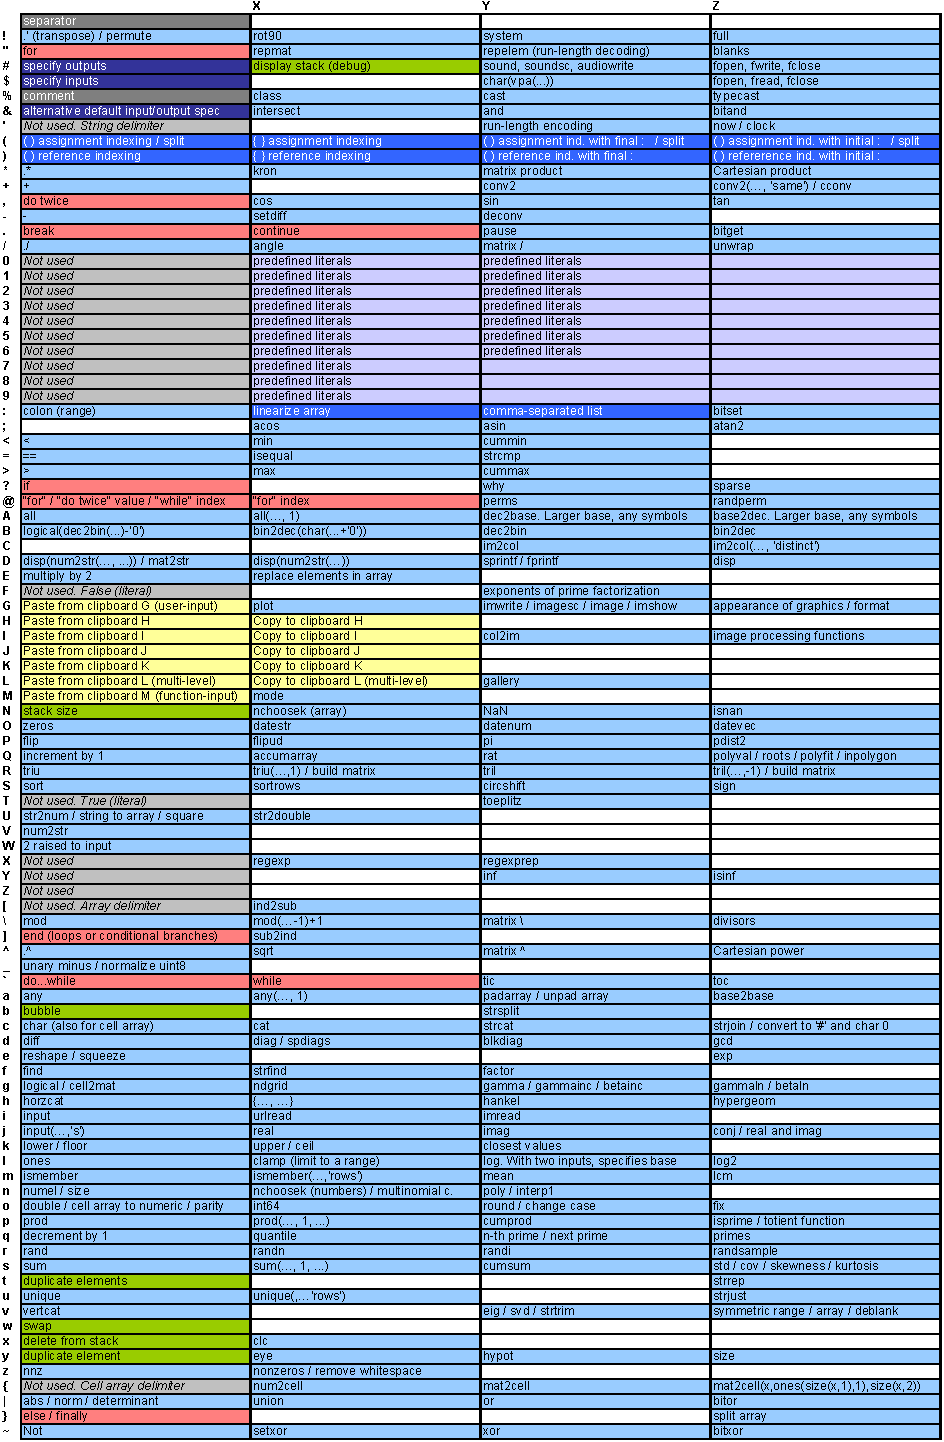
\includegraphics[scale=.82, clip]{functionTable/function_table}\\[5mm]% *!*
\hspace{3mm}\includegraphics[scale=.75, clip]{functionTable/function_table_legend}% *!*
\label{tab: function table}%
\end{table}

Table \ref{tab: function consumption} summarizes function behaviour regarding their consumption of inputs and of input/output specifications, and their overwriting the function-input clipboard.
\begin{table}
\centering
\caption{Behaviour of functions regarding consumption of inputs, consumption of input/output specifications and overwriting of function-input clipboard}
\label{tab: function consumption}
\begin{tabular}{|l|c|c|c|}
\esptab
\hline
\multicolumn{1}{|p{3cm}}{ } & \multicolumn{1}{|p{3cm}}{Consume inputs} & \multicolumn{1}{|p{3cm}|}{Consume input/ output specifications} & \multicolumn{1}{|p{3cm}|}{Overwrite function-input clipboard} \\ \hline\hline
Normal & Yes & Yes & Yes$^a$ \\ \hline
Meta & Yes & No & No\\ \hline
Stack rearranging & No & Yes & No \\ \hline
Clipboard & No & Yes & No \\ \hline
\end{tabular}
\vspace{-2mm}
\flushleft
\footnotesize{$^a$ If the function call has inputs}
\end{table}

\begin{pending}
Some functions I didn't include, and the reasons why:
\begin{itemize}
\item
\matlab+true+, \matlab+false+ functions; they can be done with \matlab+zeros+ and \matlab+ones+ (which are included) followed by conversion to \matlab+logical+ or by negation (each is just one character).
\item
\matlab+ipermute+: I don't think it's used often; and can be substituted by \matlab+permute+.
\item
\matlab+ndims+: it can be realized in two characters with \matlab+size+ followed by \matlab+numel+.
\item
\matlab+isempty+: I removed it because it can be done easily with \matlab+numel+ followed by logical negation.
\item
\matlab+length+. I followed \user{@chappjc}'s advice\footnote{\url{https://web.archive.org/web/20150915161950/http://stackexchange.com/users/3302774/chappjc}}: ``Never use \matlab+length+. Ever.''
\item
I initially thought it would be cool to have function equivalent to \matlab+eval+ in MATL. But it would be hard to implement, and probably not very useful anyway.
\item
\matlab+cellstr+: function \matlab+mat2cell(x, ones(size(x,1),1), size(x,2), ..., size(x,ndims(x)))+ exists. It's a generalization of \matlab+cell2str+ that also works for numeric and logical values, and for any number of dimensions.
\item
\matlab+shiftdim+: it seems unnecessary with \matlab+permute+.
\item
\matlab+iscolumn+, \matlab+isvector+ etc: they can be realized with \matlab+size+, and are not much used anyway, I think.
\item
\matlab+issorted+: it can be easily realized by comparing with the result of \matlab+sort+. Of course \matlab+issorted+ would be more time-efficient, but time efficiency is not the main purpose of code golf.
\item
\matlab+rem+: having \matlab+mod+ is probably enough.
\item
matrix inverse: not used very often; and can be done with matrix power, or with \matlab+eye+ and matrix division. 
\item
\matlab+rank+, matrix pseudoinverse, matrix decompositions: probably too specialized.
\item
\matlab+isequaln+: not used very often, is it?
\item
\matlab+swapbytes+: too specialized. Or is it worth including it?
\item
\matlab+factorial+: it can be done with \matlab+:+ and \matlab+prod+.
\item
\matlab+bitshift+, \matlab+bitcmp+: other bit-wise functions have been included. These two can be easily done with arithmetic operations.
\item
\matlab+strcmpi+: there's \matlab+strcmp+.
\item
\matlab+convmtx+: \matlab+convmtx(x,n)+ can be realized as \matlab+conv2(x, eye(n))+.
\item
\matlab+histcounts+ / \matlab+histc+: \matlab+histc+ would be a little redundant; compare \matlab+histc(x,unique(x))+ with \matl{8\#u} or \matl{SY'}; or compare \matlab+histc(x,y)+ with \matl{!=s}. Besides, MATLAB's \matlab+histc+ is deprecated and replaced by \matlab+histcounts+. The latter works differently; and I preferred the old \matlab+histc+'s behaviour: given \matlab+x = [10 20 30 20 30]+, \matlab+histcounts(x,unique(x))+ gives \matlab+[1 4]+ whereas \matlab+histc(x,unique(x))+ gives \matlab+[1 2 2]+.
\end{itemize}

%Remove these?
%\begin{itemize}
%\item
%\end{itemize}

\end{pending}


\section{The MATL compiler}

\subsection{Usage}

The official MATL compiler is written in MATLAB. It takes a source program in MATL and produces an output (compiled) program that is run in MATLAB. It requires version R105b or newer, although most of the functionality probably works in older versions too. The compiler also works on Octave 4.0 or newer; see \S\ref{parte: compatibility with Octave}. In addition, online compilers are available; see \S\ref{parte: online}.

The compiler can be used in any of the following ways:
\begin{itemize}
\item
\matlab+matl -options program+, or\ \matlab+matl -options 'program'+ (command syntax);
\item
\matlab+matl('-options','program')+ (function syntax).
\end{itemize}
In either case, the first input specifies processing options, starting with the character \matlab+-+; and the second input is a string or character array that contains the MATL program, or the name of a text file where the MATL program is stored. Both input arguments are optional.

The \parte{first input} argument can specify the following options for the \matl{matl} command:
\begin{itemize}
\item
\matlab+p+: parse. Writes parsed program, with one line for each statement and using indenting, in text file \matl{MATLp.txt}.
\item
\matlab+l+: listing. The parsed MATL program listing is shown on screen with one line for each statement and using indenting. Implies \matlab+p+.

\emph{Two} single-digit numeric options can be used to specify the indenting base (number of spaces to be included before any statement) and the indenting step (number of additional spaces for each nesting level). Default values are $4$ and $2$ respectively. If only one numeric option is provided, it is interpreted as the indenting base.

If a \emph{third} numeric option is provided, it is interpreted as the minimum number of spaces before comment symbol. A comment symbol is included at the end of each line, with all comment symbols vertically aligned and separated at least the specified number of spaces from the corresponding statement. This is useful for adding explanations to the code.

Numeric options can be digits \matlab+0+, \ldots, \matlab+9+; or they can be \emph{capital} letters \matlab+A+, \matlab+B+, \ldots, \matlab+Z+, which are interpreted as numbers $10$ (\matlab+A+), $11$ (\matlab+B+), \ldots, $35$ (\matlab+Z+).

File \matl{MATLp.txt} containing the parsed program uses the indenting step, but not the indenting base.

If options \matlab+c+, \matlab+r+ or \matlab+d+ have also been provided, the \matlab+matl+ command stops at this point and waits for a key press before continuing, in order to give the user time to see or copy the displayed listing.
\item
\matlab+e+: listing with comments. It's like option \matlab+l+ but automatic comment texts are added depending on the statement. These provide a good starting point to explain what the code does. Implicit statements (see \S\ref{parte: implicit actions}) are also indicated, as comments only.

In addition to the three numeric options used for option \matlab+l+, a \emph{fourth} number can be specified (using capital letters $10$, $11$, \ldots). This is interpreted as the number of spaces between comment symbols and comment text. If less than four numeric options are provided, the rest take their default values. The third and fourth numeric options have default values $6$ and $1$ respectively.

File \matl{MATLp.txt} doesn't include comments.

As happens with \matlab+l+, if options \matlab+c+, \matlab+r+ or \matlab+d+ have been provided in addition to \matlab+e+, the \matl{matl} command stops at this point and waits for a key press before continuing.
\item
\matlab+c+: compile. Produces a \matlab+.m+ file called \matlab+MATLc.m+ that can be run in MATLAB. Implies \matlab+p+.
\item
\matlab+r+: run. Runs the compiled program in MATLAB. Implies \matlab+p+ and \matlab+c+. If an error occurs in the program, the error message includes a link to open the parsed MATL file at the line of the statement that caused the error.
\item
\matlab+d+: debug. Runs the compiled program in MATLAB in debug mode. Implies \matlab+p+ and \matlab+c+. Breakpoints are set at the beginning of (the MATLAB code corresponding to) each MATL statement, to allow step-by-step execution. The variable editor is opened to show the MATL stack (variable \matlab+STACK+), input and output specifications (\matlab+S_IN+ and \matlab+S_OUT+), and clipboard contents (\matlab+CB_H+, \ldots, \matlab+CB_L+; \matlab+CB_G+; \matlab+CB_M+).

(For debugging see also function \matl{X\#} in Section \ref{parte: stack rearranging functions}).
\item
\matlab+f+: file. Indicates that the second input argument will not be MATL code, but the name of a file containing the code.
\item
\matlab+v+: verbose. Causes the compiler to provide detailed information about what it's doing.
\item
\matlab+h+: help. provides command-line help.
\item
\matlab+o+: online. This option is used in online compilers. It produces the following changes:
\begin{itemize}
\item
removes the default input prompts;
\item
doesn't generate file \matl{defout};
\item
forbids functions that read files or URL's;
% fread, imread, urlread
\item
forbids functions that write to files;
% fwrite
\item
forbids functions that evaluate arbitrary MATLAB functions or system commands.
% feval, system
\end{itemize}
\end{itemize}

If no options are provided (or only option \matlab+f+ is provided), the \matlab+matl+ program defaults to \matlab+-r+ (or \matlab+-rf+).

The \parte{second input} argument is a string that represents one of the following, depending on the selected options:
\begin{enumerate}
\item
\label{case: 2nd input: code}
The program code (options \matlab+p+, \matlab+l+, \matlab+e+, \matlab+c+, \matlab+r+, \matlab+d+);
\item
\label{case: 2nd input: file}
The name of a file containing the program code (option \matlab+f+);
\item
\label{case: 2nd input: help}
Search text to get help (option \matlab+h+).
\end{enumerate}
If the program code, file name or search text have spaces or other symbols that cause MATLAB to misinterpret the string, it needs to be enclosed in quotation marks; and then quotation marks contained within the string need to be duplicated.

In cases \ref{case: 2nd input: code} and \ref{case: 2nd input: file} the second input argument may be omitted. In this event the \matlab+matl+ command waits for input from the keyboard containing the MATL program or the file name. The MATLAB prompt is changed to a space followed by a single \matlab+>+ symbol, which indicates MATL input mode. A program may be entered in a single line or in several lines (\comp{Enter} key), and the end of the program is indicated by a blank line (\comp{Enter} key twice). A file name is entered in a single line.

In case \ref{case: 2nd input: help}, if no string is provided as second input, general help about \matlab+matl+ options is displayed. If a string is provided, it may contain the name of a MATL statement, or arbitrary search text. In the former case the information about that statement will be printed. In the latter, the search is based on case-insensitive partial matching with descriptions of MATL statements (which include equivalent MATLAB function names) and with automatic comment texts.

Examples:
\begin{itemize}
\item
\matlab+matl+: waits for user input, and runs the program represented by that input. Files \matl{MATLp.txt} and \matlab+MATLc.m+ are produced.
\item
\matlab+matl '10:"@D']+: runs the program \matl{10:"@D]}. Files \matl{MATLp.txt} and \matlab+MATLc.m+ are produced.
\item
\matlab|matl -d I4+|: runs the program \matl{I4+} in debug mode (quotation marks are needed because the code contains a space). Files \matl{MATLp.txt} and \matlab+MATLc.m+ are produced.
\item
\matlab|matl -cf file.txt|: compiles the program contained in file \comp{file.txt} and produces files \matl{MATLp.txt} and \matlab+MATLc.m+.
\item
\matlab|matl('-l82v', myProgram)|: parses the program held in character array \matlab+myProgram+, shows the parsed result without automatic comments, using the numeric options for indenting, and produces file \matl{MATLp.txt}. Detailed information about the process is also shown on screen.
\item
\matlab|matl -e0291 '1t8:"yy+'|: parses the program provided as string input (code for the Fibonacci sequence given in \S\ref{parte: examples of programs}) and shows the parsed result with automatic comments, using the numeric options for indenting. The parsed file \matl{MATLp.txt} is also produced. The result printed on screen is as shown in Figure~\ref{fig: code with automatic comments}.
\item
\matlab+matl -h ismember+ would produce the result shown in Figure~\ref{fig: help}.
\end{itemize}

\begin{figure}
\begin{small}
\begin{Verbatim}
    1        % number literal
    t        % duplicate elements
    8        % number literal
    :        % range; vector of equally spaced values
    "        % for
      y      % duplicate element
      y      % duplicate element
      +      % addition (element-wise, singleton expansion)
             % (implicit) end
             % (implicit) convert to string and display
\end{Verbatim}
\end{small}
\caption{Example of parsed code with automatic comments}
\label{fig: code with automatic comments}
\end{figure}

\begin{figure}
\begin{small}
\begin{Verbatim}[commandchars=\\\{\}]
    \textbf{m}   true for set member
        2--4 (2);  1--2 (1)
        \textbf{ismember}. It also works for cell arrays with numeric content, or
        with mixed char/numeric content. See also \textbf{Xm}
    \textbf{Xm}  true for set member, row-wise
        2--3 (2);  1--2 (1)
        \textbf{ismember(..., 'rows', ...)}. See also \textbf{m}
\end{Verbatim}
\end{small}
\caption{Example of command-line help}
\label{fig: help}
\end{figure}


\subsection{Structure}
\label{parte: compiler structure}

The \matlab+matl+ program consists of a \parte{main function}, \matlab+matl+, which calls three other functions, corresponding to the parser, compiler, and runner/debugger.

The \parte{parse function}, \matlab+matl_parse+, separates the program into statements. It includes the array checking referred to in page \pageref{parte: array checking}. Optionally it calls a display function, \matlab+matl_disp+, to print the listing of parsed code on screen. The output of the parser is a MATLAB struct array \matlab+S+ in which each entry is a statement, with fields describing the source code of the statement, the statement type and other information useful for the compiler.

The \parte{compile function}, \matlab+matl_compile+, generates MATLAB code corresponding to each statement: literals, functions and control flow statements.

Each function is defined by the MATLAB code that the compiler generates for that function. That code is divided into \emph{preamble}, \emph{function body} and \emph{postamble}. Most of the preamble and postamble code is common to different groups of functions: take inputs from stack, push results onto stack, delete \matl{\$} and \matl{\#} specifications). The function body, as well as some parameters to be used in the preamble and postamble, are specific to each function, and define what the function actually does.

Functions are defined by means of a \emph{function definition file}, \matlab+funDef.txt+. It is a tab-separated plain text file that for each function contains the function body (directly as MATLAB code) and information that controls how the preamble and postamble code should be generated. This information includes allowed and default numbers of inputs and outputs, and whether the inputs should be consumed (deleted from the stack). The file also contains the text used in automatic comments.

One of the things the preamble does is to define how many outputs the function must produce (whether specified by a previous \matl{\#} statement or by default). The function is then responsible to follow that indication. The preamble code inserted by the compiler depends on the information obtained from the function definition file.

The maximum and minimum number of allowed outputs for each function are fixed numbers specified in the function definition file. For the default number of outputs there are three possibilities:
\begin{itemize}
\item
Most commonly it is also a \emph{fixed number} indicated in the function definition file. This number is read by the compiler to generate the appropriate preamble code.
\item
For some functions, the default number of outputs cannot be determined at compile-time. Consider for example the function \matl{H}, which pastes the contents of clipboard H. Its default number of outputs is the number of elements contained by the clipboard, and thus can only be determined at run-time. In the function definition file this parameter is defined by a \emph{string} that gets directly inserted into the compiled code, and will thus be run. The string can refer to the run-time information it needs, such as number of elements in the clipboard.
\item
For a small set of functions, the default number of outputs is very difficult to compute even at run-time before the function is actually executed. For example, the function \matl{X)}, which applies \matlab+{...}+ reference indexing, produces a default number of elements that depends in a complicated manner on the input array size and on the input indices (specially if \matlab+end+-based indexing is used). In this case the default number of elements will be determined after the function has finished its computations. This is indicated in the function definition file by a \emph{negative} number as default number of outputs. This signals that it's the responsibility of the function at run-time to compute the default number of outputs and produce that many outputs, or to produce the specified number of outputs if it exists.
\end{itemize}

The postamble will discard some of the function outputs if the output specification is a logical array.

The function definition file is processed by a \matlab+genFunDef+ function, which generates a \emph{function definition struct array}, \matlab+F+, to be used by the compiler. This array contains the same information as the text file, and is saved into a \matlab+funDef.mat+ file for future use. When the compiler encounters a function in the MATL parsed code, it looks it up in array \matlab+F+ and generates the compiled (MATLAB) code accordingly. To speed up compilation, the generation of struct array \matlab+F+ is only done when the function definition file is found to be newer than the processed file \matlab+funDef.mat+; otherwise the  latter is loaded.

For functions that generate predefined literals, these are specified on a separate \emph{predefined literal file}, \matlab+preLit.txt+. It is a plain text file that for each function defines a set of key-value pairs. This is processed by a \matlab+genPreLit+ function, which generates a \emph{predefined literal struct array}, \matlab+L+, to be used by the compiler. This array contains the same information as the text file, and is saved into a \matlab+preLit.mat+ file for future use.

Lines of compiled code are stored in a cell array of strings \matlab+C+, from which the compiled file \matlab+MATLc.m+ will be written.

The function definition file and predefined literal file centralize all information about functions. This allows to define new functions without actually modifying the compiler code.

The \parte{run function}, \matlab+matl_compile+, executes the compiled program. If an error is found, an error message is issued with a link to the MATL statement that generated the error. In debug mode it inserts breakpoints and opens relevant variables (taking advantage of MATLAB's \matlab+openvar+).

The \parte{help function}, \matlab+matl_help+, provides command-line help. It uses a struct array \matlab+H+ that contains help information for all MATL functions and statements. This struct array is generated from the function definition file, the predefined literal file and additional information by a \matlab+genHelp+ function, and is stored in file \matlab+help.mat+.


\section{Compatibility with Octave}
\label{parte: compatibility with Octave}

The compiler can also run on Octave, which is a free alternative to MATLAB. Version 4.0.0 or newer is required, although most of the functionality probably works in older versions too.

Although MATLAB and Octave have a large degree of similarity, compatibility between them is not total. This has some implications that are described in the following.


\subsection{Compiler}

The debug mode of the compiler uses MATLAB's \matlab+openvar+ function to visualize the stack, clipboards and input/poutput specifications. This can't be done in Octave, because \matlab+openvar+ doesn't exist.

Octave allows the \matlab+"+ symbol as string delimiter, in addition to \matlab+'+. This implies that MATL programs that include \matlab+"+ need to be enclosed in quotation marks, in addition to those that include \matlab+'+. Note that MATL only uses \matlab+'+ as string delimiter.

An internal aspect of the compiler is that Octave randomly initializes the random number generators automatically, so the compiled code doesn't need to do it.


\subsection{MATL functions}

The definitions of MATL functions are based on MATLAB. If there are differences between a MATLAB function and the corresponding Octave function, the corresponding MATL function is defined following that of MATLAB. This means that the compiler should reproduce that behaviour even when working on Octave, in order to achieve consistent results of MATL programs.

The choice of MATLAB over Octave, admittedly arbitrary, is based on the fact that the author has more experience with MATLAB, and by no means is meant to suggest any of them is better than the other. In any case, differences between MATLAB and Octave functions are few and small, so a programmer used to Octave will not have difficulties using MATL functions.

The compiler should ensure consistent behaviour of MATL programs regardless of the underlying platform being MATLAB or Octave. In the cases when inconsistencies between MATLAB and Octave have been identified, the compiler has been programmed to correct them, if feasible. The exceptions are cases where the correction would be too difficult or when the difference is unimportant (for example, because it occurs using a function with inputs for which behaviour is undocumented).

The way the compiler deals with differences between MATLAB and Octave is as follows. If an Octave function \matlab+foo+ behaves differently from the corresponding MATLAB function, the compiled file \matlab+MATLc.m+ in Octave, which is a function, includes a subfunction that intercepts Octave's \matlab+foo+. This subfunction applies the needed modifications, and usually includes a call to Octave's original \matlab+foo+ via a \matlab+builtin+ statement. With this approach, the definitions in the MATL function definition file (\matlab+funDef.txt+) are the same for MATLAB and for Octave. In other words, the definitions assume MATLAB, and any deviations that might be caused by Octave are dealt with by the compiler.

Similarly, if a MATLAB function doesn't exist in Octave, the compiler includes it as a subfunction in the compiled file.

These compatibility functions are defined in separate files in a \emph{compatibility folder}, called \matlab+compatibility+. Each file is read as text by the compiler, if needed, to insert it as a subfunction in the compiled code.

The following list describes the cases where a discrepancy between a MATLAB and an Octave function has been detected, and indicates if the compiler addresses this or not. In most cases Octave 4.0.0 is assumed. Some of these differences may not exist in newer Octave versions.
\begin{itemize}
\item
\matlab+num2str+ behaves differently in Octave and in MATLAB\footnote{\url{http://stackoverflow.com/q/34483961/2586922}}. The compiler tries to achieve consistent behaviour, adapting the compiled code to give the same output on MATLAB and on Octave in the most common cases.
\item
\matlab+im2col+ behaves differently in Octave and in MATLAB when the block size exceeds the array size. For example, \matlab+im2col(1:8, [2 1])+ outputs \matlab+[]+ in MATLAB, and gives an error in Octave.

\matlab+im2col+ allows char input in MATLAB, but not in Octave.

Another difference exists regarding 3D input arrays. For example, the code \matlab+im2col(cat(3, magic(3), -magic(3)), [1 2])+ gives different output in MATLAB and in Octave. Apparently MATLAB collapses all dimensions of the input array beyond the first.

The above have been fixed. The compiler enforces MATLAB's behaviour when working in Octave.
\item
MATLAB's \matlab+im2col+ ignores the third and subsequent components of the second input: \matlab+im2col(1:8, [1 2 3 4])+ gives the same result as \matlab+im2col(1:8, [1 2 3 4])+. On the other hand, Octave gives an error.

With the \matlab+'distinct'+ option the behaviour is reversed: MATLAB gives an error, and Octave produces a result filled with zeros.

These differences aren't addressed in the compiler, because they are cases that are probably outside the intended use of \matlab+im2col+.
\item
\matlab+spiral+ doesn't exist in Octave. The compiler defines it as part of the compiled code if needed.
\item
\matlab+triu+, \matlab+tril+ with \matlab+[]+ and a nonzero number as inputs give an error in Octave. This has been corrected so that they return \matlab+[]+ as in MATLAB.
\item
\matlab+unique+ in Octave behaves differently than in recent MATLAB versions (it behaves like in old MATLAB versions). For the purposes of the compiler this function is modified so that it finds the first occurrence of each element, not the last; and second and third outputs are always column vectors.

Support for the \matlab+'stable'+ flag has been added.
\item
In \matlab+union+, \matlab+intesect+, \matlab+setdiff+, \matlab+setxor+: support for the \matlab+'stable'+ flag has been added, only in the single-output case.
\item
The second output of \matlab+ismember+ in Octave gives the index of the last occurrence, not the first as in recent versions of MATLAB. Also, it gives error when the first two inputs are char and numeric, whereas in MATLAB that works. Both issues are fixed.

In Octave 4.0 and 4.2, \matlab+ismember+ incorrectly treats complex values in inputs as their absolute values.\footnote{\url{https://savannah.gnu.org/bugs/index.php?52437}} This has been fixed.
% https://chat.stackoverflow.com/transcript/message/40084076#40084076
\item
\matlab+randsample+ with scalar first input produces a row vector in Octave, instead of a column vector as in MATLAB. This has been fixed in the compiler, forcing a column vector in Octave in that case.
\item
Octave's \matlab+nchoosek+, unlike MATLAB's, requires first input to be numeric. This has been fixed, so that it can be a one-dimensional character array or cell array.
\item
Octave's \matlab+vpa+ displays unwanted output. This hasn't been solved; however, it only happens in the first call to a symbolic function.
\item
When using Octave's \matlab+vpa+, conversion from symbolic to char looses precision. This is solved by converting the output of Octave's \matlab+vpa+ to string using \matlab+pretty+ (instead of \matlab+char+). This introduces unwanted whitespace in the beginning, middle and end of the string.
% Ejemplo: pretty(vpa(1, 100))
There may also be wanted whitespace separating elements of an array.
% Ejemplo: pretty(vpa(pi:5, 100))
But it is difficult to distinguish that wanted space from unwanted one. So all whitespace is removed, which only works for scalar data.

Also, in Octave trailing decimals equal to zero are produced. This has been fixed for real numbers.
\item
Octave's \matlab+vpa+ seems to have trouble with long strings containing non-integer numbers. For example, compare the output of \matlab+vpa('1/1234567891011')+ with that of \matlab+vpa('1/.1234567891011')+. This isn't addressed by the compiler.
\item
MATLAB does not support char input to \matlab+vpa+ anymore.
% This happened on R2019a, maybe earlier. In R2017b it was supported (with a warning)
Consequently, \matlab+vpa(str2sym(...), ...)+ is needed for char input. On the other hand, Octave does not have \matlab+str2sym+, but \matlab+vpa+ allows char input representing a scalar, or  \matlab+sym+ can covert char input representing a scalar. The second option is chosen. The compiler uses \matlab+vpa(str2sym(...), ...)+ for char input in the compiled code, but defines \matlab+str2sym+ to call \matlab+sym+ in Octave.
\item
Octave does not have \matlab+str2sym+. Conversion from string to symbolic is done using \matlab+sym+ instead. However, this seems to only handle strings representing scalars.
% Cuando Octave tenga str2sym quiz� se podr� hacer esa conversi�n.
\item
\matlab+sum+ and \matlab+mean+ don't support the \matlab+'omitnan'+ flag in Octave. This has been added.
\item
\matlab+diff+ and \matlab+mod+ don't allow char inputs in Octave. This has been fixed.
\item
Null assignment with less indices than dimensions works differently in MATLAB and in Octave. The code \matlab+x = cat(3,[1 2; 3 4],[1 2; 3 4]); x(:,2) = [];+ produces the result \matlab+[1 1 2; 3 3 4]+ in MATLAB (trailing dimensions are collapsed), but gives \matlab+cat(3, [1;3], [1;3])+ in Octave (no collapsing). This difference isn't addressed by the compiler.
\item
\matlab+dec2bin+ and \matlab+dec2base+ don't allow empty inputs or char inputs in Octave. This has been fixed.
\item
\matlab+hypergeom+ doesn't exist in Octave. This is partly addressed by the compiler. The function is computed either by direct sum (when some of the numerator coefficients is a non-positive integer, in which case the sum is finite) or using a third-party function\footnote{\url{http://www.mathworks.com/matlabcentral/fileexchange/5616-generalized-hypergeometric-function}}, which only works for certain ranges of input values.
\item
Octave's \matlab+disp+, unlike MATLAB's, produces some output for empty input. This has been fixed.
\item
Octave's \matlab+str2func+ works in the form \matlab+y = str2func('max')+, but not in the form \matlab+y = str2func('@(x) max(x)')+, unlike MATLAB's. This has been fixed. (This function is necessary for MATL's equivalent of \matlab+accumarray+.)
\item
In Octave arrays of type \matlab+char+ cannot be converted to \matlab+logical+. This has been fixed.
\item
The three-input version of \matlab+circshift+ doesn't exist in Octave. Also, Octave requires, unlike MATLAB, that the number of elements of the second input doesn't exceed the number of dimensions of the first. This has been fixed.
\item
In Octave, \matlab+pdist2+ allows fewer distance functions than \matlab+pdist+ does. This is solved (not very efficiently) by calling \matlab+pdist+, if needed, with the vertically concatenated inputs, and from the result extracting the desired values.
\item
\matlab+max+ and \matlab+min+ don't allow first and second inputs of type char in Octave. This has been solved.
%\item
%Octave's \matlab+strncmp+ outputs \matlab+false+ if the third input exceeds string length even if the strings are equal, whereas %MATLAB's outputs \matlab+true+. This has been solved.
% ^^ `strncmp` has been removed from MATL (it didn't seem very useful)
%\item
%MATLAB always displays \matlab+char(0)+ as a space. In Octave, on the other hand, the output is system-dependent. For example, on Windows 7 it produces a space, whereas on Linux and OS X it produces no output. To ensure a unique (and perhaps more useful) behaviour, \matlab+char(0)+ is forced to be displayed as a space when running in Octave.
%http://chat.stackoverflow.com/transcript/message/29729521#29729521
% ^^ This has changed. Now many characters below 32 (not just 0) are replaced by a space; and this is done also in MATLAB, not just in Octave, to assure consistent behaviour regardless of terminal or browser. So I indicate this in the help of functions D, XD, ZD, rather than here, because this section is for things specific to Octave.
\item
Some functions in MATLAB automatically convert input to \matlab+double+ if needed, and in Octave don't. This has been solved. These functions include \matlab+cumsum+, \matlab+cumprod+, \matlab+kron+.
\item
Octave's \matlab+datestr+ with input format \matlab+16+ (\matlab+'HH:MM PM'+) produced hour numbers greater than \matlab+12+. This was initially corrected. Then an Octave patch\footnote{\url{https://savannah.gnu.org/bugs/index.php?50673}} came out that corrects a different issue related to rounding, and that apparently incorporates the correction for input format \matlab+16+ too. So the function from that patch is used.
\item
MATLAB's \matlab+regexp+ and \matlab+regexprep+ produce empty outputs or do nothing, respectively, if the regular expression is invalid; whereas Octave's give an error. This has been solved.
\item
MATLAB's \matlab+regexprep+ accepts a numeric value as fourth input, whereas Octave's doesn't. This is partly addressed as follows: if fourth input is equal to $1$ in Octave it is replaced by \matlab+'once'+, so that at least that one works.
\item
Octave's \matlab+strsplit+ gives an error when trying to split on \matlab|+|. This has been fixed.
% The `+` needed escaping; this has been modified in the source code
\item
Octave's \matlab+str2num+ gives an error with certain inputs. This has been fixed.
\item
In Octave, \matlab+str2num+ with input \matlab+'e'+ produces number $e$ (and similarly for inputs like \matlab+'[1; e]'+). In MATLAB it produces an empty array, that is, the string is not recognized as a number. This difference is addressed by the compiler, so that the behaviour in Octave is as in MATLAB.
\item
In MATLAB, \matlab+str2double+ linearizes char input into a row, whereas in Octave it doesn't. This has been solved.
\item
MATLAB's \matlab+imshow+, by default, produces one screen pixel for each image pixel. On the other hand, Octave's \matlab+imshow+ scales the image on the screen. This has been partly fixed, so image pixels and screen pixels coincide. ``Partly'' means that the fix only works in some platforms, for reasons unknown (at least by me).
\item
Octave's \matlab+mat2str+ doesn't handle char input. This has been fixed for inputs containing printable ASCII chars.
\item
Octave's \matlab+strcat+ doesn't remove trailing space when the input is a single string. This has been fixed.
\item
\matlab+y = [1 3 5; 2 4 6]; y([1 3 5]) = []+ gives \matlab+[2 4 6]+ in MATLAB but \matlab+[2; 4; 6]+ in Octave.
% (4.0.0)
The pattern seems to be: if \matlab+~isvector(y)+ MATLAB reshapes as a row, whereas Octave reshapes as a column. This is addressed by explicitly reshaping as a row in that case.
\item
Matlab's \matlab+disp+ displays \matlab+char(0)+ as space on any platform. Octave displays it as either space, or narrow space, or nothing.\footnote{\urlG} MATL's display functions replace \matlab+char(0)+ (and other chars with codepoint below $32$) by space before calling \matlab+disp+.
\item
In MATLAB, \matlab+input(..., 's')+ (unevaluated input) interprets input consisting of only spaces as empty input. This doesn't happen in Octave. This difference has not been addressed.
\item
In MATLAB, \matlab+sprintf('%1.1g', 0.25)+ gives \matlab+0.3+ on Windows (round away from zero) and \matlab+0.2+ on Linux (banker's rounding). In Octave it gives \matlab+0.2+ both on Windows and on Linux.\footnote{\url{https://savannah.gnu.org/bugs/index.php?51515}} These differences have not been addressed.
\item
\matlab+char+ implicitly rounds down in MATLAB, and rounds to closest in Octave. This difference has been addressed by enforcing MATLAB's behaviour.
Octave's \matlab+mode+ doesn't handle char input. This has been fixed.
\item
Octave treats ranges specially to save memory\footnote{\url{https://www.gnu.org/software/octave/doc/v4.2.0/Ranges.html}}. When applying function \matlab+nnz+ to a range an error occurs. This has been fixed.
\end{itemize}


\section{Running MATL online}
\label{parte: online}

MATL code can be executed online in the following two awesome platforms. Many thanks to \user{@Dennis} and \user{@Suever} for providing them!
\begin{itemize}
\item
\user{@Dennis}' \emph{Try It Online} platform\footnote{\url{https://tio.run/\#matl}}. The online compiler runs on Octave. Text output is displayed normally, and graphical output is displayed (with limitations) by Octave's fancy ASCII-graph capabilities.
\item
\user{@Suever}'s \emph{MATL Online} interpreter\footnote{\url{https://matl.suever.net/}}. This platform is MATL-specific and allows real-time text output, graphical output and documentation search, among other features.
\end{itemize}


\section{Example programs explained}
\label{parte: example programs explained}

In the following, the examples given in \S\ref{parte: examples of programs} are explained. This serves to illustrate some of the features of MATL. See \S\ref{parte: table of functions} and \S\ref{parte: list of functions} for the detailed definition of the functions involved.


\subsection{Example 1: infinite loop}

Code: \matl{`T]}.

This is a ``do-while'' loop. This type of loop is always entered at least once. Within the loop, \matl{T} pushes a \matlab+true+ literal to make sure the loop condition is met. This literal is consumed and the program proceeds with the next iteration, indefinitely.

The code could be shortened to \matl{`T}, because MATL automatically closes loops at the end of the program if they have not been previously closed.


\subsection{Example 2: first 10 Fibonacci numbers}

Code: \matl{1t8:"yy+}.

The first statement, \matl{1}, pushes number $1$ onto the stack. \matl{t} makes a copy of it, so the stack now contains \matl{1}, \matl{1}. Statement \matl{8} pushes an $8$. Function \matl{:} by default takes one input, and transforms the top of the stack, which is \matl{8}, into vector \matl{[1 2 3 4 5 6 7 8]}. So the stack now contains, bottom to top: \matl{1}, \matl{1}, \matl{[1 2 3 4 5 6 7 8]}.

Statement \matl{"} begins a ``for'' loop applied on vector \matl{[1 2 3 4 5 6 7 8]}. Thus there will be $8$ iterations, each corresponding to an entry of this vector. Since the vector is consumed by \matl{"}, at the beginning of the first iteration the stack contains \matl{1}, \matl{1}. The loop body begins with \matl{y}, which duplicates the second-top element from the stack and pushes the copy onto the top. So \matl{yy} duplicates the top two elements (like \matl{2\$t} would, but saving one character). Then \matl{+} computes their sum to produce \matl{2}.

Note that the \matl{]} that closes the \matl{"} loop is missing. This is allowed, because it is implicitly inserted by MATL at the end of the program.

So at the end of the first iteration the stack contains \matl{1}, \matl{1}, \matl{2}. The second iteration again operates on the top $2$ elements, \matl{1}, \matl{2}, to produce their sum \matl{3}; and so on. The initial \matl{1}, \matl{1} remain in the stack as the first $2$ members of the Fibonacci sequence, and the $8$ loop iterations produce the next $8$ Fibonacci numbers, to complete the total of $10$.

At the end of the program, the function \matl{XD} is implicitly called. By default this function displays all elements in the stack, from bottom to top.


\subsection{Example 3: unique characters from string in original order}

Code: \matl{ju}.

\matl{j} inputs a string (without any prompt string by default). The second statement is function \matl{u}, which corresponds to \matlab+unique+ with the \matlab+'stable'+ flag by default. This function takes as input the string typed by the user to produce the desired result, which is displayed by the implicit final call to \matl{XD}.



\subsection{Example 4: unique characters from string in original order, manual approach}

Code: \matl{jtt!=XRa\textasciitilde{})}. This produces the same result as in the previous example, but without using \matl{u}.

\matl{j} inputs a string. This is duplicated twice by \matl{tt}, and the last copy is transposed by \matl{!}. Function \matl{=} consumes both copies (normal and transposed) and compares them element-wise with singleton expansion, producing a logical matrix. Entry $(m,n)$ of this matrix is \matlab+true+ if and only if the $m$-th character of the input string equals the $n$-th character. Thus the matrix is symmetric and contains \matlab+true+ values along the diagonal. The stack now conbtains the original string and the comparison matrix.

\matl{XR} corresponds to \matlab+triu(..., 1)+, and thus keeps the part of the matrix above the diagonal, making all other entries \matlab+false+. This will assure that only duplicates with respect to \emph{preceding characters} are detected.

\matl{a} corresponds to \matlab+any+, with $1$ input by default. The result is a logical row vector with a \matlab+true+ at entry $m$ if and only if the upper-triangular matrix produced by the previous function (\matl{XR}) has at least a \matl{true}  value at column $m$; that is, if that character was a duplicate of a preceding character. Function \matl{\textasciitilde{}} negates this logical vector, so that \matlab+true+ indicates characters that should be kept. The stack now contains the original string and this logical vector. Function \matl{)}, which takes $2$ inputs by default, indexes the string with the logical vector to produce the desired result, which will be implicitly displayed.


\section{Acknowledgments}

Thanks to the following people (in alphabetical order) for their contributions:
\begin{itemize}
\item
\user{@AndrasDeak} for his very extensive testing of the compiler. Also for his help (together with \user{@beaker}) regarding a bug in Octave's \matlab+ismember+ function with complex inputs.
% https://chat.stackoverflow.com/transcript/message/40084076#40084076
\item
\user{@beaker} for a helpful discussion
% http://chat.stackoverflow.com/transcript/message/26114026#26114026
that led me to reconsider including a form of \matlab+end+-based indexing, for telling me about Octave's \matlab+repelems+ function, and for pointing out several errata. Also for his help (together with \user{@AndrasDeak}) regarding a bug in Octave's \matlab+ismember+ function with complex inputs.
% https://chat.stackoverflow.com/transcript/message/40084076#40084076
\item
\user{Ben Barrowes} for his function \matlab+genHyper+.
\item
\user{Conor O'Brien} for his suggestion to have a function essentially equivalent to \matl{35*c} but shorter.
% https://codegolf.stackexchange.com/questions/138883/fractal-cathedral/138886#comment340831_138886
\item
\user{@David} for finding a good implementation of the ``$n$-th prime'' function, as well as some errata in this document. Also for suggesting that \matl{G} should take implicit input if needed, and for finding a bug in Octave's \matlab+datestr+ function.
\item
\user{@Dennis} for hosting MATL in his wonderful \emph{Try It Online} platform\footnote{\url
{http://tryitonline.net}}. Also for suggesting modular indexing, and bit-wise operations with negative values.
\item
\user{@DJMcMayhem} for finding some errata, and also for suggesting that a square-power and a divisors function be added.
%http://chat.stackexchange.com/transcript/message/30482878#30482878
%https://chat.stackexchange.com/transcript/message/33065597#33065597
\item
\user{@EriktheOutgolfer} for finding some errata in the documentation.
% https://chat.stackexchange.com/transcript/message/44392192#44392192
\item
\user{@excaza} for his suggestion regarding the hypergeometric function.
\item
\user{@flawr} for his suggestions, including the ``$n$-th prime'' function, ``shuffle'' function and implicit input of data, and for finding several bugs.
\item
\user{@FryAmTheEggman} for helpful comments that led to improvements related to \matlab+nchoosek+.
\item
\user{@Giuseppe} for finding a bug in \matl{u}.
\item
\user{@H.PWiz} for correcting a typo in the documentation.
% https://chat.stackexchange.com/transcript/message/42323700#42323700
\item
\user{@pragmatist1} for suggesting the use of a regular expression to check contents of array literals.
% http://codegolf.stackexchange.com/questions/74789/vandermonde-determinant#comment181478_74799
\item
\user{@quartata} for his suggestions related to the determinant function.
\item
\user{@RainerP} for a helpful discussion related to ``if'' branches and the automatic function clipboard.
%http://codegolf.stackexchange.com/a/68987/36398
\item
\user{@rayryeng} for coming up with the initial idea\footnote{\urlF} and for his invaluable help in getting MATL to work online. Also for his suggestion to include predefined constants, for reading an early version of this document and suggesting changes, and for his support with this project.
\item
\user{@Sanchises} for noticing bugs in \matl{Za} (base conversion), in \matl{Y@} (variations without repetition),
% https://chat.stackexchange.com/transcript/message/40439254#404392
in the Octave compatibility function for \matl{X\textasciitilde{}} (\matlab+setxor+), the latter of which also affected other functions, and for finding another problem in that function, which turned out to be related to a weird Octave bug with vertical concatenation;
% https://chat.stackexchange.com/transcript/message/41392103#41392103
% https://savannah.gnu.org/bugs/index.php?52542
for noticing a difference with \matlab+char+'s implicit rounding in MATLAB and in Octave;
% https://chat.stackexchange.com/transcript/message/41158178#41158178
for suggesting to include \matlab+expm+ (matrix exponential) and to generalize matrix power as a sum over different exponents;
% https://chat.stackexchange.com/transcript/message/41206681#41206681
for finding a bug in the parser, which incorrectly identified \matl{]} or \matl{\}} within strings as closing symbols for array literals;
% https://chat.stackexchange.com/transcript/message/42555761#42555761
for suggesting to generalize \matl{z} for cell arrays;
% https://chat.stackexchange.com/transcript/message/49993614#49993614
and for suggesting that MATL should have a symbolic data type.
% https://chat.stackexchange.com/transcript/message/52437616#52437616
\item
\user{@Steadybox} for finding a bug in Octave's \matlab+nnz+ function when applied to a range.
% Comments in https://codegolf.stackexchange.com/a/155943/36398
\item
\user{@Suever} for his help in finding several differences between Octave and MATLAB,
% regarding the $0$ character, as well as the \matlab+max+ and \matlab+min+ functions;
% concatenation of chars and logical doesn't work in Matlab
and for finding a bug in MATL's extension of \matlab+reshape+, in \matl{YG} (\matlab+imshow+), and in Octave's compatibility patch for \matl{u} and \matl{Xu} (\matlab+unique+). Also for suggesting that \matl{\&} should produce a ``secondary default'' input/output specification, adapted to each function (my initial idea was to simply have it increase the number of inputs by $1$), and for his valuable help in finding the most appropriate secondary specification for each function, including a very useful script to get information from MATL answers posted in the Programming Puzzles and Code Golf site. Thanks too for his suggestion to have automatic input transposition for single-input versions of addition, multiplication and other functions, and for his suggestion which led to the name ``element-wise indexing''. And, specially, thanks for creating and maintaining the awesome \emph{MATL Online} platform\footnote{\url{https://matl.suever.net/}}.
% http://chat.stackoverflow.com/transcript/message/29716461#29716461
% http://chat.stackoverflow.com/transcript/message/29717853#29717853
% http://chat.stackoverflow.com/transcript/message/29835862#29835862
% http://chat.stackoverflow.com/transcript/message/30154628#30154628
% http://codegolf.stackexchange.com/questions/82981/leyland-numbers#comment202388_82995
\item
\user{@sundar} for prompting me to clarify that strings are understood as row vectors of chars in MATL; for several corrections in the documentation, for a correction in \matl{Z\{}; for a correction in \matl{S}; and for suggesting the \matl{Zx} function, two-input char mode for \matl{Yo} and a modification in \matl{Yb}.
% https://chat.stackexchange.com/transcript/message/46222193#46222193
% https://codegolf.stackexchange.com/questions/166527/decoding-the-kaadi-system/168021#comment405995_168021
% https://chat.stackexchange.com/transcript/message/45568841#45568841
% https://chat.stackexchange.com/transcript/39466?m=45568698#45568698
\end{itemize}


\begin{appendices}

\section{Detailed function definitions}
\label{parte: list of functions}

MATL functions are defined in Table~\ref{tab: funDef}.

The notation for allowed, default and alternative numbers of inputs and outputs is as follows. Consider for example the \matl{p} function (which corresponds to MATLAB's \matlab+prod+). Then ``\matl{p}\ \ 1--3 (1 / 2)\ 1'' means that this function can accept $1$ to $3$ inputs, with $1$ as default and $2$ as secondary default; and produces $1$ output. This notation may be abbreviated if the number of inputs or outputs is unbounded or is fixed: ``\matl{(}\ \ 3-- (3 / 4)\ \ 1'' means that the number of inputs can be any integer starting at $3$, the number of outputs is always $1$; the default is $3$ inputs, and the secondary default is $4$ inputs.


\begin{small}
\begin{longtable}{lllp{.67\textwidth}}
\caption{Function definitions}\\ % It seems "\\" is needed in this case
%\esptab
\label{tab: funDef}
\matl{!} & 1--2 (1 / 2) & 1 & If $1$ input: \matlab+.'+ (\matlab+transpose+), or \matlab+permute(..., [2 1 ...])+ for multidimensional arrrays. If $2$ inputs: \matlab+permute+. If the second input is 1, 2 or 3 it indicates which dimension is not permuted for a 3D array; that is, it corresponds to [1 3 2], [3 2 1] or [2 1 3] respectively \\
\matl{X!} & 1--2 (2) & 1 & \matlab+rot90+ \\
\matl{Y!} & 1 & 0--2 (2) & \matlab+system+ \\
\matl{Z!} & 1 & 1 & \matlab+full+ \\
\matl{X"} & 2-- (3) & 1 & \matlab+repmat+ \\
\matl{Y"} & 2-- (2 / 3) & 1 & \matlab+repelem+ (run-length decoding). With $2$ inputs: if the first or second inputs are empty the output is empty. Else, the second input is linearized if needed; and if the first or second input is shorter than the other, entries are repeated cyclically to match lengths \\
\matl{Z"} & 1 & 1 & \matlab+blanks+. It allows vector input, and in that case it produces a matrix or multidimensional array \\
\matl{X\#} & 0 & 0 & display stack as a cell array \\
\matl{Y\#} & 2-- (2 / 3) & 0 & (i) With $2$ inputs: \matlab+sound+. If second input is \matl{T}, it is interpreted as \matl{44100}. If second input is \matl{F}, it is interpreted as \matl{44100} and \matlab+audiowrite+ is called instead of \matlab+sound+, with file name \matlab+'audio.wav'+. (ii) With $3$ inputs: if third input is a truthy scalar, \matlab+soundsc+ is called with the first two inputs. If third input is a numeric vector of size $2$, \matlab+soundsc+ is called with the three inputs. In both cases, \matl{T} in second input is interpreted as \matl{44100}. If third input is a string, it defines a file name, and \matlab+audiowrite+ is called with that file name and the other two inputs. (iii) With more than $3$ inputs: \matlab+audiowrite+ is called using the third input as file name. Further inputs specify parameter-value pairs. \matl{T} in second input is interpreted as \matl{44100}.  \\
\matl{Z\#} & 1--3 (1 / 2) & 0 & Writes first input to file \comp{inout}, creating it if necessary. If the file exists, by default its previous contents are overwritten. If the input is a numeric or char array each entry is treated as a raw byte and written. Behaviour is undefined for entries exceeding $255$. If the input is a cell array, the contents of each cell are written, with a byte $10$ (representing newline) in between. With $2$ inputs: second input specifies file name; it is converted to char is necessary; if empty defaults to \comp{inout}. With $3$ inputs: third input specifies whether previous contents of the file should be kept \\
\matl{X\$} & 1-- (2 / 2) & 0-- (1) & execute Matlab function specified by first input, using the rest of the inputs as arguments. \\
\matl{Y\$} & 1--2 (2) & 1 & \matlab+char(vpa(...))+ \\
\matl{Z\$} & 0--1 (0 / 1) & 1 & Reads bytes from specifed file. Each individual byte is then converted to a char, and the output is a row vector of char. If $0$ inputs or empty input: file name is \comp{inout}. \\
\matl{X\%} & 1 & 1 & class of input (\matlab+class+ with one input) \\
\matl{Y\%} & 2--3 (2) & 1 & \matlab+cast+. This function allows strings in second input to be replaced by numbers, as follows: 1: \matlab+'uint8'+, 2: \matlab+'int8'+, 3: \matlab+'uint64'+, 4: \matlab+'int64'+, 5: \matlab+'uint16'+, 6: \matlab+'int16'+, 7: \matlab+'uint32'+, 8: \matlab+'int32'+, 9: \matlab+'double'+, 10: \matlab+'single'+ \\
\matl{Z\%} & 2 & 1 & \matlab+typecast+. This function allows strings in second input to be replaced by numbers, as follows: 1: \matlab+'uint8'+, 2: \matlab+'int8'+, 3: \matlab+'uint64'+, 4: \matlab+'int64'+, 5: \matlab+'uint16'+, 6: \matlab+'int16'+, 7: \matlab+'uint32'+, 8: \matlab+'int32'+, 9: \matlab+'double'+, 10: \matlab+'single'+ \\
\matl{X\&} & 2--4 (2 / 3) & 1--3 (1) & \matlab+intersect+. Uses the \matlab+'stable'+ flag by default. If one input is char and the other is numeric, the latter is converted to char. This function allows flag strings in third and subsequent inputs to be replaced by numbers, as follows: 1: \matlab+'rows'+, 2: \matlab+'stable'+, 3: \matlab+'sorted'+ \\
\matl{Y\&} & 0-- (2 / $^\ddagger$) & 1 & \matlab+&+ (\matlab+and+), element-wise with singleton expansion \\
\matl{Z\&} & 2--3 (2) & 1 & \matlab+bitand+ (bitwise 'and'), element-wise with singleton expansion. If first or second inputs are \matlab+char+ they are converted to \matlab+double+. \matlab+double+ inputs are rounded. If the inputs are \matlab+double+ they can have negative values, and in that case they must be in the range from \matlab+-2^52+ up to \matlab+2^52-1+. \sa \matl{Z|}, \matl{Z\textasciitilde{}} \\
\matl{Y'} & 1 & 2 (2 / 2nd) & run-length encoding (inverse of \matlab+repelem+). Input may be an array or cell array. Numeric values must be finite \\
\matl{Z'} & 0--1 (0 / 1) & 1 & \matlab+now+. With $1$ input: the input should be numeric with values from 1 to 6, which are used as indices into the output of \matlab+clock+ \\
\matl{(} & 3-- (3 / 4) & 1 & assignment \matlab+( )+ indexing. Null assignment (\matlab+x(...) = []+) can only be done with a single index. \sa \matl{Y(}, \matl{Z(} \\
\matl{X(} & 3-- (3) & 1 & assignment \matlab+{ }+ indexing \\
\matl{Y(} & 2-- (3) & 1 & assignment \matlab+(..., :)+ indexing. Null assignment (\matlab+x(..., :) = []+) can only be done with a single index (in addition to the implicit colon). \sa \matl{(}, \matl{Z(} \\
\matl{Z(} & 2-- (3) & 1 & assignment \matlab+(:, ...)+ indexing. Null assignment (\matlab+x(:, ...) = []+) can only be done with a single index (in addition to the implicit colon). \sa \matl{(}, \matl{Y(} \\
\matl{)} & 2-- (2) & 1--2 (1 / 2) & reference \matlab+( )+ indexing. If $2$ outputs: only one input index can be used. The second output produces the "complementary" array \matlab+y=x; y(ind)=[]+, where \matlab+y+ and \matlab+ind+ are the inputs. \sa \matl{Y)}, \matl{Z)} \\
\matl{X)} & 2-- (2) & 0-- ($^\bigtriangledown$) & reference \matlab+{ }+ indexing \\
\matl{Y)} & 1-- (2) & 1--2 (1 / 2) & reference \matlab+(..., :)+ indexing. If $2$ outputs: only one input index can be used. The second output produces the "complementary" array \matlab+y=x; y(ind,:)=[]+, where \matlab+y+ and \matlab+ind+ are the inputs. \sa \matl{)}, \matl{Z)} \\
\matl{Z)} & 1-- (2) & 1--2 (1 / 2) & reference \matlab+(:, ...)+ indexing. If $2$ outputs: only one input index can be used. The second output produces the "complementary" array \matlab+y=x; y(:,ind)=[]+, where \matlab+y+ and \matlab+ind+ are the inputs. \sa \matl{)}, \matl{Y)} \\
\matl{*} & 1-- (2 / 1) & 1 & \matlab+.*+ (\matlab+times+), element-wise with singleton expansion. If $1$ input: a second input is used given by the first transposed \\
\matl{X*} & 2 & 1 & \matlab+kron+ \\
\matl{Y*} & 2 & 1 & matrix product, \matlab+*+ (\matlab+mtimes+) \\
\matl{Z*} & 1-- (2 / $^\ddagger$) & 1 & Cartesian product. Given a number $n$ of arrays of possibly different sizes, generates an $n$-column matrix whose rows describe all combinations of elements taken from those arrays \\
\matl{+} & 1-- (2 / 1) & 1 & \matlab|+| (\matlab+plus+), element-wise with singleton expansion. If $1$ input: a second input is used given by the first transposed \\
\matl{Y+} & 2--3 (2 / 3) & 1 & \matlab+conv2+. Doesn't allow two-vector and one matrix mode. Converts first two inputs to \matlab+double+. This function allows flag strings in third and subsequent inputs to be replaced by numbers, as follows: 1: \matlab+'same'+, 2: \matlab+'valid'+, 3: \matlab+'full'+. \sa \matl{Z+} \\
\matl{Z+} & 2--3 (2 / 3) & 1 & (i) If $2$ inputs: \matlab+conv2(..., 'same')+. (ii) If $3$ inputs: \matlab+cconv+. Non-vector inputs are linearized into column vectors. The output is of type \matlab+double+. Integer inputs are guaranteed to give exact integer results, up to \matlab+double+ data type limitations. (i,ii) Inputs are converted to \matlab+double+. \sa \matl{Y+} \\
\matl{X,} & 1 & 1 & \matlab+cos+ \\
\matl{Y,} & 1 & 1 & \matlab+sin+ \\
\matl{Z,} & 1 & 1 & \matlab+tan+ \\
\matl{-} & 1--2 (2 / 1) & 1 & \matlab+-+ (\matlab+minus+), element-wise with singleton expansion. If $1$ input: a second input is used given by the first transposed \\
\matl{X-} & 2--4 (2 / 3) & 1--2 (1) & \matlab+setdiff+. Uses the \matlab+'stable'+ flag by default. If one input is char and the other is numeric, the latter is converted to char. This function allows flag strings in third and subsequent inputs to be replaced by numbers, as follows: 1: \matlab+'rows'+, 2: \matlab+'stable'+, 3: \matlab+'sorted'+. \sa \matl{X\textasciitilde{}} \\
\matl{Y-} & 2 & 1--2 (1 / 2) & \matlab+deconv+ \\
\matl{Y.} & 0--1 (1) & 0 & \matlab+pause+ (without outputs) \\
\matl{Z.} & 2--3 (2) & 1 & \matlab+bitget+. If first input is \matlab+char+ it is automatically converted to \matlab+double+ \\
\matl{/} & 2 & 1 & \matlab+./+ (\matlab+rdivide+), element-wise with singleton expansion \\
\matl{X/} & 1 & 1 & \matlab+angle+ \\
\matl{Y/} & 2 & 1 & right matrix division, \matlab+/+ (\matlab+mrdivide+) \\
\matl{Z/} & 1--3 (1) & 1 & \matlab+unwrap+ \\
\matl{X0} & 1 & 1 & predefined literal depending on input \\
\matl{Y0} & 1 & 1 & predefined literal depending on input \\
\matl{X1} & 1 & 1 & predefined literal depending on input \\
\matl{Y1} & 1 & 1 & predefined literal depending on input \\
\matl{X2} & 1 & 1 & predefined literal depending on input \\
\matl{Y2} & 1 & 1 & predefined literal depending on input \\
\matl{X3} & 1 & 1 & predefined literal depending on input \\
\matl{Y3} & 1 & 1 & predefined literal depending on input \\
\matl{X4} & 1 & 1 & predefined literal depending on input \\
\matl{Y4} & 1 & 1 & predefined literal depending on input \\
\matl{X5} & 1 & 1 & predefined literal depending on input \\
\matl{Y5} & 1 & 1 & predefined literal depending on input \\
\matl{X6} & 1 & 1 & predefined literal depending on input \\
\matl{Y6} & 1 & 1 & predefined literal depending on input \\
\matl{X7} & 1 & 1 & predefined literal depending on input \\
\matl{X8} & 1 & 1 & predefined literal depending on input \\
\matl{X9} & 1 & 1 & predefined literal depending on input \\
\matl{:} & 1--3 (1 / 2) & 1 & \matlab+colon+ (with three inputs \matlab+x+, \matlab+y+, \matlab+z+ produces \matlab+x:y:z+; with two inputs \matlab+x+, \matlab+y+ produces \matlab+x:y+). If one input: produces \matlab+1:x+, or \matlab+' ':x+ if \matlab+x+ is char. For a single cell-array input, the contents of the cell array are interpreted as the actual inputs. \\
\matl{X:} & 1 & 1 & linearize to column array (index with \matlab+(:)+) \\
\matl{Y:} & 1 & 0-- ($^\triangle$) & generate comma-separated list from cell array (index with \matlab+{:}+) and push each element onto stack \\
\matl{Z:} & 2--4 (3) & 1 & \matlab+bitset+. If first input is \matlab+char+ it is automatically converted to \matlab+double+ \\
\matl{X;} & 1 & 1 & \matlab+acos+ \\
\matl{Y;} & 1 & 1 & \matlab+asin+ \\
\matl{Z;} & 2 & 1 & \matlab+atan2+, element-wise with singleton expansion \\
\matl{<} & 1--2 (2 / 1) & 1 & \matlab+<+ (\matlab+lt+), element-wise with singleton expansion. If $1$ input: a second input is used given by the first transposed \\
\matl{X<} & 1--3 (1) & 1--2 (1 / 2nd) & \matlab+min+. If $2$ inputs: element-wise with singleton expansion. With more than $2$ inputs, the second is replaced by \matl{[]}. This function does not support flags \matlab+'omitnan'+ or \matlab+'includenan'+. Output is \matlab+char+ if input is. \sa \matl{X>}, \matl{Xl} \\
\matl{Y<} & 1--3 (1 / 2) & 1 & \matlab+cummin+. Output is \matlab+char+ if input is. \sa \matl{Y>} \\
\matl{=} & 1--2 (2 / 1) & 1 & \matlab+==+ (\matlab+eq+), element-wise with singleton expansion. If $1$ input: a second input is used given by the first transposed \\
\matl{X=} & 0-- (2 / $^\ddagger$) & 1 & \matlab+isequal+. Works for any number of inputs \\
\matl{Y=} & 2 & 1 & \matlab+strcmp+. If first or second inputs are numeric they are converted to char \\
\matl{>} & 1--2 (2 / 1) & 1 & \matlab+>+ (\matlab+gt+), element-wise with singleton expansion. If $1$ input: a second input is used given by the first transposed \\
\matl{X>} & 1--3 (1) & 1--2 (1 / 2nd) & \matlab+max+. If $2$ inputs: element-wise with singleton expansion. With more than $2$ inputs, the second is replaced by \matl{[]}. This function does not support flags \matlab+'omitnan'+ or \matlab+'includenan'+. Output is \matlab+char+ if input is. \sa \matl{X<}, \matl{Xl} \\
\matl{Y>} & 1--3 (1 / 2) & 1 & \matlab+cummax+. Output is \matlab+char+ if input is. \sa \matl{Y<} \\
\matl{Y?} & 0 & 1 & answer why. Sort of \\
\matl{Z?} & 1--6 (3) & 1 & \matlab+sparse+. If $3$ inputs and third input is \matlab+char+, the output is converted to \matlab+char+ \\
\matl{Y@} & 1--2 (1 / 2) & 1 & If $1$ input: \matlab+perms+. If $2$ inputs: variations (without repetition). In either case, the results are sorted \\
\matl{Z@} & 1--3 (1 / 2) & 1 & \matlab+randperm+ (produces a row vector as output). If $3$ inputs: third input indicates number of permutations, each on a different row. If first input is char it is interpreted as population (not as size) \\
\matl{A} & 1--2 (1 / 2) & 1 & \matlab+all+. \sa \matl{XA} \\
\matl{XA} & 1 & 1 & \matlab+all(..., 1)+. \sa \matl{A} \\
\matl{YA} & 2--3 (2 / 3) & 1 & (i) \matlab+dec2base+. (ii) If second input has more than one element: it defines the symbols, which can be characters or numbers. The number of symbols defines the base, which can exceed $36$. (iii) If second input is a negative number \matlab+-n+: it is interpreted as symbols \matlab+0:n-1+ (case ii). (i, ii) Base \matl{0} is interpreted as \matl{10}, \matl{1} as \matl{16}, \matl{F} as \matl{0:9}, \matl{T} as \matl{0:15}. \sa \matl{ZA}, \matl{Za} \\
\matl{ZA} & 2 & 1 & (i) \matlab+base2dec+. (ii) If second input has more than one element: it defines the symbols, which can be characters (case-sensitive) or numbers. The number of symbols defines the base, which can exceed $36$. (iii) If second input is a negative number \matlab+-n+: it is interpreted as symbols \matlab+0:n-1+ (case ii). (i, ii, iii) Non-recognized digits are ignored. Base \matl{0} is interpreted as \matl{10}, \matl{1} as \matl{16}, \matl{F} as \matl{0:9}, \matl{T} as \matl{0:15}. \sa \matl{YA}, \matl{Za} \\
\matl{B} & 1--2 (1 / 2) & 1 & \matlab|logical(dec2bin(...)-'0')|. \sa \matl{YB} \\
\matl{XB} & 1 & 1 & \matlab|bin2dec(char(logical(...)+'0'))|. Works also for cell array input. \sa \matl{ZB} \\
\matl{YB} & 1--2 (1 / 2) & 1 & \matlab|dec2bin|. \sa \matl{B} \\
\matl{ZB} & 1 & 1 & \matlab|bin2dec|. \sa \matl{XB} \\
\matl{YC} & 2--4 (2) & 1 & \matlab+im2col+. If the second input is a scalar \matlab+n+, it is transformed into \matlab+[1 n]+ if the first input is a row vector, or to \matlab+[n 1]+ otherwise. First input can also be a cell array. \sa \matl{ZC} \\
\matl{ZC} & 2--3 (2) & 1 & \matlab+im2col(..., 'distinct')+. If the second input is a scalar n, it is transformed into [1 n] if the first input is a row vector, or to [n 1] otherwise. First input can also be a cell array. \sa \matl{YC} \\
\matl{D} & 0-- (1) & 0--1 (0 / 1) & (i) With $0$ outputs: If $1$ input: \matlab+disp(num2str(..., '%.15g '))+. If several inputs: \matlab+disp(num2str(eachInput,lastInput))+, where \matlab+eachInput+ loops over all inputs but the last. In either case, (nested) cell arrays are (recursively) unboxed in linear order. Most characters below 32 are replaced by space. (ii) With $1$ output: \matlab+mat2str+. Empty arrays are always shown as \matlab+[]+, \matlab+''+ or \matlab+{}+. Most input characters below 32 are replaced by space. Cell arrays are converted to string representation too. Optional second, third and fourth inputs respectively specify column separator, row separator and whether the separators should be used for non-cell arrays too. Second and third output are converted to char is needed. \sa \matl{XD}, \matl{YD}, \matl{ZD} \\
\matl{XD} & 0-- ($^\ddagger$ / 1) & 0 & \matlab+disp(num2str(eachInput, '%.15g '))+, where \matlab+eachInput+ loops over all inputs. (Nested) cell arrays are (recursively) unboxed in linear order. Most characters below 32 are replaced by space. \sa \matl{D}, \matl{YD}, \matl{ZD} \\
\matl{YD} & 1-- (2 / 1) & 0--2 (1 / 0) & \matlab+sprintf+ with format string as last input. If $0$ outputs: prints to screen using \matlab+fprintf(...)+. \sa \matl{D}, \matl{XD}, \matl{ZD} \\
\matl{ZD} & 0-- (1) & 0 & \matlab+disp+ for each input. For char input, most characters below 32 are replaced by space. \sa \matl{D}, \matl{XD}, \matl{YD} \\
\matl{E} & 1 & 1 & \matlab|(...)*2| \\
\matl{XE} & 3 & 1 & With numeric or char inputs, replace in first input all occurrences of each element of the second input by the corresponding element of the third input. The third input may be longer than the second, and then the extra elements are ignored. Or it may have a single element, and then it is implicitly replicated. Output has the same class and size as the first input. If the three inputs are cell arrays of strings (the second may also be a string instead of a cell array of strings), each string of the first input is considered atomic, that is, replacing is based on whole strings. If the first input is a cell array and the others are numeric or char, replacing is done on each cell's contents as if the cell's contents were the first input \\
\matl{YF} & 1 & 1--2 (1 / 2) & (i) With $1$ output: exponents of prime factor decomposition, without skipping primes. If the input is a numeric array it is linearized, and each result is in an output row. If any entry in the input is negative, the absolute value is taken, and the output contains only non-zero exponents. (ii) With $2$ outputs: first output gives the prime factors, second gives the exponents. Primes that are not factors are skipped, as are their zero exponents. If any entry in the input is negative, the absolute value is taken, and all intermediate primes are included, possibly with zero exponents. \sa \matl{Yf} \\
\matl{ZF} & 1--3 (1 / 2) & 1 & (i) With $1$ or $2$ inputs: \matlab+nfft+. If first input is a vector and second input is a scalar, a $1$ is prepended or appended to the second input according to the vector orientation (so the result is the same as that of \matlab+fft+). (ii) With $3$ inputs: \matlab+fft+ \\
\matl{G} & 0--1 ($^\sqcup$ / 0) & 0-- ($^\sqcap$) & paste from user-input clipboard G. If $0$ input arguments: addresses all levels. If $1$ input argument: addresses specified level. In either of those cases, if clipboard G has no levels one user-input is implicitly taken to fill the first level \\
\matl{XG} & 1-- (1 / 2) & 0 & \matlab+plot+. Calls \matlab+drawnow+ to update figure immediately. With one input, or with several inputs the second of which is a string: if the first input is complex (even with zero imaginary part), \matlab+axis equal+ is also called. \\
\matl{YG} & 2-- (2 / 3) & 0 & \matlab+imwrite+, \matlab+imagesc+, \matlab+image+ or \matlab+imshow+. (i) If last input is a scalar: \matlab+0+ corresponds to \matlab+imwrite+, \matlab+1+ to \matlab+imagesc+, \matlab+2+ to \matlab+image+ and \matlab+3+ to \matlab+imshow+. The corresponding function is called with the remaining inputs. (ii) If last input is numeric or logical and not a scalar: \matlab+imshow+ is called with all inputs. (iii) If last input is char: \matlab+imwrite+ is called with all inputs. (i, iii) For \matlab+imwrite+, the first input of type char is interpreted as file name. If it has no extension '.png' is added; if it's empty it is replaced by 'image.png'; and if non existent 'image.png' is used as final input. (i, ii, iii) For \matl{imshow} and \matl{imwrite}, if the second input is logical it is converted to \matlab+double+. If it is numeric, has the shape of a colormap, and has some entry greater than $1$, it is normalized by converting to \matlab+uint8+, then to \matlab+double+, and then dividing by $255$. For \matlab+imagesc+ and \matlab+image+, the function call is followed by \matlab+axis ij, axis image+. For \matlab+imagesc+, \matlab+image+ and \matlab+imshow+, \matlab+drawnow+ is called to update figure immediately \\
\matl{ZG} & 1-- (2 / 3) & 0--1 (0) & Depending on numeric last input, calls a graphic function or \matlab+format+ with the remaining inputs.  $0$: \matlab+format+.  $1$: \matlab+axis+. Calls \matlab+drawnow+ to update figure immediately. Flag strings in first to second-last inputs can be replaced by numbers, as follows: 1: \matlab+'equal'+, 2: \matlab+'image'+, 3: \matlab+'square'+, 4: \matlab+'ij'+, 5: \matlab+'xy'+, 6: \matlab+'normal'+, 7: \matlab+'off'+, 8: \matlab+'on'+, 9: \matlab+'tight'+, 10: \matlab+'manual'+, 11: \matlab+'fill'+, 12: \matlab+'auto'+, 13: \matlab+'vis3d'+.  $2$: \matlab+colormap+. If the first input is numeric, has the shape of a colormap, and has some entry greater than $1$, it is normalized by converting to \matlab+uint8+, then to \matlab+double+, and then dividing by $255$. With $0$ outputs, calls \matlab+drawnow+ to update figure immediately.  $3$: \matlab+hold+. Flag strings in first input can be replaced by numbers, as follows: 1: \matlab+'on'+, 2: \matlab+'off'+. \\
\matl{H} & 0 & 0-- ($^\dagger$) & paste from clipboard H \\
\matl{XH} & 0-- (1 / 2) & 0 & copy to clipboard H \\
\matl{I} & 0 & 0-- ($^\dagger$) & paste from clipboard I \\
\matl{XI} & 0-- (1) & 0 & copy to clipboard I \\
\matl{YI} & 3--4 (3 / 4) & 1 & \matlab+col2im+. Uses \matlab+'distinct'+ option by default. Second and third inputs may be scalars, and then they are interpreted as numbers of columns. Third input may be a two-vector with product less then the number of elements of first input, and then it is appropriately scaled. This function allows flag strings in fourth input to be replaced by numbers, as follows: 1: \matlab+'distinct'+, 2: \matlab+'sliding'+ \\
\matl{ZI} & 1-- (2 / 3) & 1-- (1) & Depending on numeric last input, calls an image processing function with the remaining inputs.  $0$: \matlab+imfill+. If first input is logical or numerical it is converted to char.  $1$: \matlab+bwlabeln+.  $2$: \matlab+imdilate+. This function allows second input to be number $4$, $5$, $8$ or $9$, which is interpreted as the corresponding neighbourhood mask.  $3$: \matlab+imerode+. This function allows second input to be number $4$, $5$, $8$ or $9$, which is interpreted as the corresponding neighbourhood mask. \\
\matl{J} & 0 & 0-- ($^\dagger$) & paste from clipboard J \\
\matl{XJ} & 0-- (1) & 0 & copy to clipboard J \\
\matl{K} & 0 & 0-- ($^\dagger$) & paste from clipboard K \\
\matl{XK} & 0-- (1) & 0 & copy to clipboard K \\
\matl{L} & 1 & 0-- ($^\dagger$) & paste from multi-level clipboard L. Input specifies level \\
\matl{XL} & 1-- (2 / 3) & 0 & copy to multi-level clipboard L. Last input specifies level \\
\matl{YL} & 1-- (2 / 3) & 1-- (1) & \matlab+gallery+ with matrix name as last input. Also includes \matlab+magic+, \matlab+hilb+, \matlab+invhilb+, \matlab+hadamard+, \matlab+pascal+, \matlab+spiral+. This function allows some strings in last input to be replaced by numbers, as follows:  1: \matlab+'spiral'+, 2: \matlab+'pascal'+, 3: \matlab+'magic'+, 4: \matlab+'hadamard'+, 5: \matlab+'circul'+, 6: \matlab+'gcdmat'+, 7: \matlab+'minij'+, 8: \matlab+'hilb'+, 9: \matlab+'invhilb'+, 10: \matlab+'tridiag'+, 11: \matlab+'ris'+ \\
\matl{M} & 1 & 0-- ($^\ast$) & paste from function-input clipboard M. Input specifies level ($1$ to $4$) or individual input ($5$ or larger) \\
\matl{XM} & 1--2 (1) & 1--3 (1) & \matlab+mode+. First input can be a cell array of strings \\
\matl{N} & 0 & 1 & number of elements in the stack \\
\matl{XN} & 2 & 1 & \matlab+nchoosek+. This interprets first input as an array (even if it is a single number). For inputs \matlab+x+ and \matlab+k+, if \matlab+x+ has less than \matlab+k+ elements or if \matlab+k+ is non-positive the result is an empty array. \sa \matl{Xn} \\
\matl{YN} & 0-- (0) & 1 & \matlab+NaN+ function. If $0$ inputs: produces literal \matlab+NaN+. \\
\matl{ZN} & 1 & 1 & \matlab+isnan+ \\
\matl{O} & 0-- (0 / 2) & 1 & \matlab+zeros+ (if $0$ inputs: produces output $0$) \\
\matl{XO} & 1--4 (2) & 1 & \matlab+datestr+ \\
\matl{YO} & 1--6 (1 / 2) & 1 & \matlab+datenum+. With $2$ inputs, if the second input is numeric it is interpreted as a format specifier as in \matlab+datestr+ \\
\matl{ZO} & 1--3 (1 / 2) & 1--6 (1) & \matlab+datevec+ \\
\matl{P} & 1--2 (1 / 2) & 1 & \matlab+flip+. \sa \matl{XP} \\
\matl{XP} & 1 & 1 & \matlab+flipud+. \sa \matl{P} \\
\matl{YP} & 0 & 1 & \matlab+pi+ \\
\matl{ZP} & 2--5 (2 / 3) & 1--2 (1) & \matlab+pdist2+. Only predefined distance functions are allowed. This function allows flag strings in the third input to be replaced by numbers, as follows:  1: \matlab+'cityblock'+, 2: \matlab+'hamming'+, 3: \matlab+'chebychev'+, 4: \matlab+'correlation'+, 5: \matlab+'cosine'+, 6: \matlab+'seuclidean'+, 7: \matlab+'minkowski'+, 8: \matlab+'mahalanobis'+, 9: \matlab+'spearman'+, 10: \matlab+'jaccard'+, 11: \matlab+'euclidean'+ \\
\matl{Q} & 1 & 1 & \matlab|(...)+1| \\
\matl{XQ} & 2--6 (3) & 1 & \matlab+accumarray+. If first input is \matlab+char+ it is converted to \matlab+double+. The third input may be omitted, and then it is interpreted as \matlab+[]+. Fourth/third argument specifies an anonymous function, as follows:  1: \matlab+'@sum'+, 2: \matlab+'@mean'+, 3: \matlab+'@(x){sort(x).'}'+, 4: \matlab+'@max'+, 5: \matlab+'@min'+, 6: \matlab+'@prod'+, 7: \matlab+'@(x){x.'}'+, 8: \matlab+'@(x){x}'+, 9: \matlab+'@(x){sort(x)}'+, 10: \matlab+'@(x)x(1)'+, 11: \matlab+'@(x)x(end)'+, 12: \matlab+'@(x){cumsum(x).'}'+, 13: \matlab+'@(x){cumprod(x)}'+, 14: \matlab+'@nansum'+, 15: \matlab+'@nanmean'+, 16: \matlab+'@nanmax'+, 17: \matlab+'@nanmin'+, 18: \matlab+'@(x){cummax(x).'}'+, 19: \matlab+'@(x){cummin(x)}'+, 20: \matlab+'@(x){cummax(x).'}'+, 21: \matlab+'@(x){cummin(x)}'+ \\
\matl{YQ} & 1--2 (1) & 1--2 (2) & \matlab+rat+ \\
\matl{ZQ} & 1--4 (2 / 1) & 1--2 (1) & (i) If $1$ input: \matlab+roots+. (ii) If $2$ inputs: \matlab+polyval+. If $3$ inputs: \matlab+polyfit+. If $4$ inputs: \matlab+inpolygon+ \\
\matl{R} & 1--2 (1 / 2) & 1 & \matlab+triu+. \sa \matl{XR}. \\
\matl{XR} & 1--2 (1 / 2) & 1 & \matlab+triu(..., 1)+. If $2$ inputs: builds an upper triangular or symmetric matrix from a vector (or from an array in linear order). Second input indicates if the diagonal is filled/not and if the matrix is made symmetric, as follows. 0: don't use diagonal, don't make symmetric. 1: use diagonal, don't make symmetric. 2: don't use diagonal, make symmetric. 3: use diagonal, make symmetric. \sa \matl{R}, \matl{ZR} \\
\matl{YR} & 1--2 (1 / 2) & 1 & \matlab+tril+. \sa \matl{ZR}. \\
\matl{ZR} & 1--2 (1 / 2) & 1 & \matlab+tril(..., -1)+. If $2$ inputs: builds a lower triangular or symmetric matrix from a vector (or from an array in linear order). Second input indicates if the diagonal is filled/not and if the matrix is made symmetric, as follows. 0: don't use diagonal, don't make symmetric. 1: use diagonal, don't make symmetric. 2: don't use diagonal, make symmetric. 3: use diagonal, make symmetric. \sa \matl{XR}, \matl{YR}. \\
\matl{S} & 1--3 (1) & 1--2 (1 / 2nd) & sort an array (\matlab+sort+) / sort an array based on another. (i) Single-array mode works like Matlab's \matlab+sort+. If $2$ inputs, a negative value of the second input corresponds to descending order. If first input is a cell array and the first cell contains a char array, the rest of the cells' contents are converted to char. (ii) If the first input is a cell array and the first cell contains a numeric array, single-array numeric mode is used. The first input is linearized if it's not a vector, and its contents are linearized for the purposes of sorting. The first input is then sorted in lexicographic order, ignoring other inputs. (iii) In two-array mode, this function takes as first $2$ inputs an array and a vector array which is not char. If the first array is not a vector it is linearized. The second vector is sorted and its order is applied to the first. An optional third input specifies direction as a string, or as a negative number in the non-singleton dimension of the second vector. The outputs are the two sorted arrays. (In two-array mode, if the two input arrays are scalar the result is the same as if the second input is interpreted as dimension, corresponding to single array mode). \sa \matl{XS} \\
\matl{XS} & 1--2 (1) & 1--2 (1 / 2nd) & \matlab+sortrows+. \sa \matl{S} \\
\matl{YS} & 2--3 (2 / 3) & 1 & \matlab+circshift+. If second input is a scalar and there's no third input, the shift is applied along the first non-singleton dimension. This function also allows first input a 2D array; third input a scalar specifying dimension; and second input a vector or array specifying the shift for each position in the other dimension \\
\matl{ZS} & 1--2 (1 / 2) & 1 & (i) With $1$ input: \matlab+sign+. (ii) With $2$ inputs: \matlab+fftshift+. Second input equal to $0$ corresponds to \matlab+fftshift+ with $1$ input \\
\matl{YT} & 1--2 (1 / 2) & 1 & \matlab+toeplitz+. Output is char if any input is \\
\matl{U} & 1 & 1--2 (1) & (i) For char input: \matlab+str2num+ with content checking. Most characters below 32 are replaced by space (as in \matl{D}). The input content is then checked. If it fails, \matlab+[]+ is returned. Else \matlab+str2num+ is applied. If that fails, the input string is evaluated. If that also fails, \matlab+[]+ is returned. The second output is supported in all cases. (ii) For numeric input: \matlab+(...).^2+ \\
\matl{XU} & 1 & 1 & \matlab+str2double+ \\
\matl{V} & 1--2 (1 / 2) & 1 & \matlab+num2str+. Uses format \matlab+'%.15g '+ by default. To get Matlab's default format use \matlab+[]+ as format specification \\
\matl{W} & 1 & 1 & \matlab+2.^(...)+. Array power (or rather exponentiation) with base $2$ \\
\matl{XX} & 2--9 (2 / 3) & 1--6 ($^\Diamond$) & \matlab+regexp+. With $2$ inputs and $1$ output: \matlab+regexp(..., ..., 'match')+. If first or second inputs are numeric they are converted to char. If they are numeric or char arrays they are linearized into a row. If they are cells their contents are converted to char. \matlab+'names'+ output is not supported. This function allows flag strings in third and subsequent inputs to be replaced by numbers, as follows: 1: \matlab+'start'+, 2: \matlab+'split'+, 3: \matlab+'end'+, 4: \matlab+'once'+, 5: \matlab+'tokenExtents'+, 6: \matlab+'tokens'+, 7: \matlab+'match'+ \\
\matl{YX} & 3--5 (3 / 4) & 1 & \matlab+regexprep+. If first, second or third inputs are numeric they are converted to char. If they are numeric or char arrays they are linearized into a row. If they are cells their contents are converted to char \\
\matl{YY} & 0-- (0) & 1 & \matlab+inf+ function. If $0$ inputs: produces literal \matlab+inf+. \\
\matl{ZY} & 1 & 1 & \matlab+isinf+ \\
\matl{X[} & 2 & 1-- ($^\triangle$) & \matlab+ind2sub+ without input restrictions \\
\matl{\textbackslash } & 2 & 1--2 (1 / 2) & \matlab+mod+, element-wise with singleton expansion. With $2$ outputs: second output is \matlab+floor(.../...)+. \sa \matl{X\textbackslash }, \matl{o} \\
\matl{X\textbackslash } & 2 & 1 & \matlab|mod(...-1, ...)+1|, element-wise with singleton expansion. \sa \matl{\textbackslash } \\
\matl{Y\textbackslash } & 2 & 1 & left matrix division, \matlab+\+ (\matlab+mldivide+) \\
\matl{Z\textbackslash } & 1 & 1 & divisors of a number. For negative input the absolute value is used \\
\matl{X]} & 3-- (3) & 1 & \matlab+sub2ind+ without input restrictions \\
\matl{\textasciicircum{}} & 2 & 1 & \matlab+.^+ (\matlab+power+), element-wise with singleton expansion \\
\matl{X\textasciicircum{}} & 1 & 1 & \matlab+sqrt+ \\
\matl{Y\textasciicircum{}} & 2 & 1 & \matlab+^+ (\matlab+mpower+) \\
\matl{Z\textasciicircum{}} & 2 & 1 & (i) Given an array and a number $n$, computes the Cartesian power of the array times itself $n$ times. (ii) If the first input is a number and the second input is an array of at least two elements, the inputs are interpreted in reverse order. When using this mode, caution is needed in case the second input (array) may become a scalar, because then mode (i) will be used. \sa \matl{Z*} \\
\matl{\_} & 1 & 1 & (i) If input is \matlab+uint8+: unary \matlab+-+ (\matlab+uminus+), that is, output is the negative of the input. (ii) If input is \matlab+uint8+: converts to \matlab+double+ and divides by $255$ \\
\matl{Y`} & 0 & 0--1 (0) & \matlab+tic+. \sa \matl{Z`} \\
\matl{Z`} & 0--1 (0) & 0--1 (1) & \matlab+toc+. \sa \matl{Y`} \\
\matl{a} & 1--2 (1 / 2) & 1 & \matlab+any+. \sa \matl{Xa} \\
\matl{Xa} & 1 & 1 & \matlab+any(..., 1)+. \sa \matl{a} \\
\matl{Ya} & 2--4 (2 / 3) & 1 & (i) \matlab+padarray+. It allows the first input to be \matlab+char+; and then the output is also \matlab+char+. If the second input is \matlab+logical+ or the pad value is \matlab+char+ they are converted to \matlab+double+. This function allows flag strings in fourth input to be replaced by numbers, as follows: 1: \matlab+'pre'+, 2: \matlab+'post'+, 3: \matlab+'both'+. (ii) If the second input contains at least one negative or complex value, the array in the first input is unpadded. The array can only have two dimensions. The second input can have one or two entries, specifying dimensions. A negative value indicates unpad along that dimension. A complex value indicates unpad along the two dimensions. The third input specifies which values are considered padding; by default $0$ \\
\matl{Za} & 3--4 (3 / 4) & 1 & Converts the number represented by input 1 from the base specified by input 2 to that of input 3. Each base can be a number or a vector. In the first case the alphabet is from 0 to that number minus 1. If the second or third input equals \matl{T} or \matl{F}, it is respectively interpreted as \matlab+' ':'~'+ (all printable ASCII chars) or \matlab+[' ':'&' '(':'~']+ (all printable ASCII chars except single quote). Non-valid digits in the first input are discarded. An optional fourth input indicates number of digits of the result. First input can be a matrix or a cell array; and then the result is a matrix in which each row corresponds to a row of the input matrix, or to a cell of the input cell array in linear order. \sa \matl{YA}, \matl{ZA} \\
\matl{b} & 0-- (3 / 4) & 0 & bubble up element in stack \\
\matl{Yb} & 1-- (1 / 2) & 1--2 (1) & (i) \matlab+strsplit+. If second input is numeric it is converted to char. This function allows flag strings in third, fifth etc inputs to be replaced by numbers, as follows: 1: \matlab+'CollapseDelimiters'+, 2: \matlab+'DelimiterType'+, 3: \matlab+'RegularExpression'+, 4: \matlab+'Simple'+. (ii) First input can be a cell array of strings, and then the result is a cell array of cell arrays of strings. Only one output is supported in this mode. (iii) First input can be numeric. In this mode only one output is supported, the default delimiter is 0, and the parameter \matlab+'CollapseDelimiters'+ can be used. The second input (delimiter) can be a single number or a numeric array, and in the latter case each element is a possible delimiter. If the first input is a row array the output will contain row arrays; otherwise it will contain column arrays \\
\matl{c} & 1-- (1) & 1 & \matlab+char+. Sparse input is first converted to full, and logical input is first converted to double. For cell array input, non-char cell contents are first converted to char \\
\matl{Xc} & 3-- (3 / $^\ddagger$) & 1 & \matlab+cat+. The dimension is the last input \\
\matl{Yc} & 1-- (2 / $^\ddagger$) & 1 & \matlab+strcat+. If not all inputs are numerical or logical, numerical or logical inputs are converted to char. If all inputs are numerical or logical the result is numerical or logical (with singleton expansion along the first dimension), and no trailing values are removed  \\
\matl{Zc} & 1--2 (1 / 2) & 1 & If cell input: \matlab+strjoin+. This function also allows input with numeric content. The first cell of the first input determines char or numeric mode. If that cell contains a char (resp. numeric) array, numeric (resp. char) contents in other cells, as well as the second input or its contents, are converted to char (resp. double). (i) Char mode corresponds to \matlab+strjoin+. (ii) Numeric mode is similar: it has a default delimiter, which is 0; or a single delimiter may be specified, which may be a scalar or an array; or a cell array of delimiters may be used. (i, ii) Both in char and in numeric mode, non-vector arrays are linearized, and the result is a row vector. Surplus delimiters are ignored. (iii) With a single, non-cell input: nonzeros are replaced by 35 (code point of \matlab+'#'+) and the result is converted to char \\
\matl{d} & 1--3 (1 / 2) & 1 & \matlab+diff+ with second and third input interchanged: second specifies dimension, third specifies difference order. \\
\matl{Xd} & 1--4 (1 / 2) & 1--2 (1) & If $1$ input and $1$ output: \matlab+diag+. Otherwise: \matlab+spdiags+, with char inputs automatically converted to \matlab+double+. With $2$ inputs and $1$ output, if the second input is \matlab+true+ it selects all diagonals from the first input \\
\matl{Yd} & 1-- (2 / $^\ddagger$) & 1 & \matlab+blkdiag+ \\
\matl{Zd} & 1--2 (2 / 1) & 1--3 (1) & \matlab+gcd+, element-wise with singleton expansion. With $1$ input and $1$ output, computes the greatest common divisor of all elements of the input \\
\matl{e} & 1-- (2 / 1) & 1 & (i) With $1$ input: \matlab+squeeze+. (ii) With more than $1$ input: \matlab+reshape+. If second input is logical, contiguous equal values indicate dimensions that will be collapsed; and a final \matlab+[]+ is implicit. If second input is a (non-logical) scalar, a final \matlab+[]+ is implicit. If size specification doesn't contain \matlab+[]+ (explicit or implicit), the first input is padded or truncated if needed; padding is done with \matlab+0+, \matlab+false+, \matlab+char(0)+ or \matlab+{[]}+ according to type of first input. If size specification contains \matlab+[]+ (explicit or implicit), the first input is padded if needed \\
\matl{Ze} & 1 & 1 & \matlab+exp+ \\
\matl{f} & 1--3 (1) & 1--3 (1 / 2) & \matlab+find+ \\
\matl{Xf} & 1--4 (2 / 1) & 1 & (i) If 2 or more inputs: \matlab+strfind+. Works also when the first input is a numeric array or a cell array of numeric arrays. In this case each numeric array is linearized, and results are row vectors. (ii) If 1 input: output is a cell array of all non-empty substrings. Works also for numeric or cell arrays \\
\matl{Yf} & 1 & 1 & \matlab+factor+. For input $1$ it returns an empty array, not $1$ like \matlab+factor+ does. For negative input, \matlab+factor+ is applied to the absolute value of the input (so input $-1$ produces $1$). \sa \matl{YF} \\
\matl{g} & 1 & 1 & (i) For non-cell input: \matlab+logical+. Works also for complex numbers, using their absolute value. (ii) For cell input: \matlab+cell2mat+ \\
\matl{Xg} & 1-- (2) & 1-- ($^\square$) & \matlab+ndgrid+ \\
\matl{Yg} & 1--3 (1) & 1 & \matlab+gamma+ / \matlab+gammainc+ / \matlab+betainc+, depending on number of inputs \\
\matl{Zg} & 1--2 (1 / 2) & 1 & \matlab+gammaln+ / \matlab+betaln+, depending on number of inputs \\
\matl{h} & 0-- (2 / $^\ddagger$) & 1 & \matlab+horzcat+. If inputs are matrices with non-matching sizes they are linearized \\
\matl{Xh} & 0-- ($^\ddagger$ / 2) & 1 & concatenate into cell array (\matlab+{..., ...}+) \\
\matl{Yh} & 1--2 (2 / 1) & 1 & \matlab+hankel+. If any input is of type char: returns char output \\
\matl{Zh} & 3 & 1 & \matlab+hypergeom+. If a numerator coefficient is a nonpositive integer the series is truncated at the first index for which a zero appears in the numerator, regardless of the denominator \\
\matl{i} & 0--2 (0) & 1 & \matlab+input+ with content checking. If $0$ inputs: uses default prompt string. \sa \matl{j}. \\
\matl{Xi} & 1--5 (1) & 1--2 (1) & \matlab+urlread+. If the input string doesn't contain \matl{'://'}, the string \matl{'http://'} is prepended \\
\matl{Yi} & 1-- (1) & 1--3 (1) & \matlab+imread+ \\
\matl{j} & 0--1 (0) & 1 & \matlab+input(..., 's')+. If $0$ inputs: uses default prompt string. \sa \matl{i} \\
\matl{Xj} & 1 & 1 & \matlab+real+ \\
\matl{Yj} & 1 & 1 & \matlab+imag+ \\
\matl{Zj} & 1 & 1--2 (1 / 2) & (i) With one output: complex conjugate (\matlab+conj+). (ii) With two outputs: real and imaginary parts (\matlab+real+, \matlab+imag+) \\
\matl{k} & 1 & 1 & \matlab+lower+ for strings or cell arrays; \matlab+floor+ for numerical arrays \\
\matl{Xk} & 1 & 1 & \matlab+upper+ for strings or cell arrays of strings; \matlab+ceil+ for numerical arrays \\
\matl{Yk} & 2 & 1--3 (1 / 3rd) & closest value in second input to each value in first input, in terms of absolute difference. For equidistant values it picks the one that appears first (in linear order) in the second input. Second output gives resulting absolute differences. Third output gives linear indices of selected elements \\
\matl{l} & 0-- (0 / 2) & 1 & \matlab+ones+ (if $0$ inputs: produces output $1$) \\
\matl{Xl} & 2--3 (2 / 3) & 1 & (i) With $2$ inputs, the minimum of the two inputs is computed, element-wise with singleton expansion. (ii) With $3$ inputs, the function computes the minimum between the first and the second, and then the maximum between that and the third, element-wise with singleton expansion. (i, ii) Output is \matlab+char+ if first input is. \sa \matl{X<}, \matl{X>} \\
\matl{Yl} & 1--2 (1 / 2) & 1 & \matlab+log+. If $2$ inputs: second input specifies logarithm base \\
\matl{Zl} & 1 & 1--2 (1) & \matlab+log2+ \\
\matl{m} & 2--4 (2) & 1--2 (1 / 2nd) & \matlab+ismember+. It also works for cell arrays with numeric content, or with mixed char/numeric content. \sa \matl{Xm} \\
\matl{Xm} & 2--3 (2) & 1--2 (1 / 2nd) & \matlab+ismember(..., 'rows', ...)+. \sa \matl{m} \\
\matl{Ym} & 1--4 (1 / 2) & 1 & \matlab+mean+. This function allows flag strings in third and subsequent inputs to be replaced by numbers, as follows: 1: \matlab+'omitnan'+, 2: \matlab+'includenan'+, 3: \matlab+'double'+, 4: \matlab+'native'+, 5: \matlab+'default'+ \\
\matl{Zm} & 1--2 (2 / 1) & 1 & \matlab+lcm+, element-wise with singleton expansion. With $1$ input, computes the least common multiple of all elements of the input \\
\matl{n} & 1 & 1-- (1 / $^\times$) & \matlab+numel+. For several outputs, or a single output other than the first, gives \matlab+size+ along those dimensions \\
\matl{Xn} & 1--2 (2 / 1) & 1 & (i) If $2$ inputs: \matlab+nchoosek+. This interprets first input as number(s). If the inputs are arrays, the function is computed element-wise with singleton expansion. For values \matlab+n+ and \matlab+k+ in first and second inputs, if \matlab+n+ is less than \matlab+k+ the result is \matlab+0+. (ii) If $1$ input: multinomial coefficient. The input contains the lower terms; their sum is the upper term. \sa \matl{XN} \\
\matl{Yn} & 1--5 (2 / 4) & 1 & (i) If $1$ input: \matlab+poly+. (ii) If $2$ or more inputs: \matlab+interp1+. With $2$ or $3$ numeric inputs, flags \matlab+'linear'+ and \matlab+'extrap'+ are assumed. \matlab+'pp'+ option not supported. A finite numeric value in the fourth input is replaced by a flag string, as follows: 1: \matlab+'linear'+, 2: \matlab+'nearest'+, 3: \matlab+'next'+, 4: \matlab+'previous'+, 5: \matlab+'spline'+, 6: \matlab+'pchip'+, 7: \matlab+'cubic'+, 8: \matlab+'v5cubic'+ \\
\matl{o} & 1--3 (1 / 2) & 1 & (i) \matlab+double+. (ii) For cell array input behaves similarly to \matlab+char+: linearizes cell array, converts cell contents to \matlab+double+ and concatenates vertically, padding if needed. By default, padding is with zeros on the right. Optional second input indicates fill side: left if it evaluates to \matlab+false+, right if it evaluates to \matlab+true+. Third optional input specifies fill value. (iii) If input is already of type \matlab+double+: \matlab+mod(..., 2)+  \\
\matl{Xo} & 1 & 1 & \matlab+int64+ \\
\matl{Yo} & 1--3 (1 / 2) & 1 & (i) For numeric arrays: \matlab+round+. Third input can be a number instead of a string, as follows: 1: \matlab+'significant'+, 2: \matlab+'decimals'+. (ii) For character arrays or cell arrays of strings: change case \\
\matl{Zo} & 1 & 1 & \matlab+fix+ \\
\matl{p} & 1--3 (1 / 2) & 1 & \matlab+prod+. If first input is \matlab+char+ it is converted to \matlab+double+. \sa \matl{Xp} \\
\matl{Xp} & 1--3 (1) & 1 & \matlab+prod(..., 1, ...)+. If first input is \matlab+char+ it is converted to \matlab+double+. \sa \matl{p}. \\
\matl{Yp} & 1--4 (1 / 2) & 1 & \matlab+cumprod+. Allows first input to be char. If $3$ numeric inputs: the third input is interpreted as a minimum which is applied after the product at each position. If $4$ numeric inputs: last two inputs are minimum and maximum respectively \\
\matl{Zp} & 1 & 1 & For input with non-negative entries: \matlab+isprime+. For input with non-positive entries: Euler's totient function for absolute value of each entry \\
\matl{q} & 1 & 1 & \matlab+(...)-1+ \\
\matl{Xq} & 2--3 (2 / 3) & 1 & \matlab+quantile+ \\
\matl{Yq} & 1 & 1 & For input with positive entries: $n$-th prime for each value $n$ in the input array. For input with non-positive entries: next prime for absolute value of each entry \\
\matl{Zq} & 1 & 1 & \matlab+primes+ \\
\matl{r} & 0-- (0 / 2) & 1 & \matlab+rand+ \\
\matl{Xr} & 0-- (0 / 2) & 1 & \matlab+randn+ \\
\matl{Yr} & 1-- (1 / 2) & 1 & \matlab+randi+. If the first input is a vector of $2$ elements it is automatically sorted. With $2$ inputs, if the second input is a scalar \matlab+n+ it is transformed into \matlab+[1 n]+ \\
\matl{Zr} & 2--4 (2 / 3) & 1 & \matlab+randsample+. Does not support stream specification \\
\matl{s} & 1--4 (1 / 2) & 1 & \matlab+sum+. This function allows flag strings in third and subsequent inputs to be replaced by numbers, as follows: 1: \matlab+'omitnan'+, 2: \matlab+'includenan'+, 3: \matlab+'double'+, 4: \matlab+'native'+, 5: \matlab+'default'+. \sa \matl{Xs} \\
\matl{Xs} & 1--3 (1) & 1 & \matlab+sum(..., 1, ...)+. This function allows flag strings in third and subsequent inputs to be replaced by numbers, as follows: 1: \matlab+'omitnan'+, 2: \matlab+'includenan'+, 3: \matlab+'double'+, 4: \matlab+'native'+, 5: \matlab+'default'+. \sa \matl{s} \\
\matl{Ys} & 1--4 (1 / 2) & 1 & \matlab+cumsum+. Allows first input to be char. Optional third and fourth numerical scalar inputs are interpreted as minimum and maximum values, which are applied after the sum at each position. These can be substituted by a 2-element numerical array as second or third input \\
\matl{Zs} & 1--4 (1 / 2) & 1 & (i) \matlab+std+. (ii) With $2$ inputs \matlab+x+, \matlab+k+ and \matlab+k+ equal to $2$ or $3$, gives \matlab+cov(x, k-2)+. (iii) With $2$ inputs \matlab+x+, \matlab+k+ and \matlab+k+ equal to $4$ or $5$, gives \matlab+skewness(x(:), k-4)+. (iv) With $2$ inputs \matlab+x+, \matlab+k+ and \matlab+k+ equal to $6$ or $7$, gives \matlab+kurtosis(x(:), k-6)+ \\
\matl{t} & 0-- (1) & 0 & duplicate elements in stack. The duplicated elements are those specified as inputs \\
\matl{Zt} & 3 & 1 & (i) If first input is char or a cell array: \matlab+strrep+. Numerical second and third inputs are converted to char. (ii) The first input can be a numerical or logical array (not a cell array of numeric or logical arrays). In this case the other inputs can be char, numeric or logical (not cell); each input array is linearized; result is a row vector; and result has the type of the third input, even if no substitutions have been actually done \\
\matl{u} & 1--4 (1) & 1--4 (1) & \matlab+unique+, with \matlab+'stable'+ option by default. It includes a fourth output with the count for each unique element. It also allows cell array input with numeric content, or mixed char/numeric content. In this case it only works with a single output, either in sorted or stable mode. This function allows flag strings in second and subsequent inputs to be replaced by numbers, as follows: 1: \matlab+'stable'+, 2: \matlab+'sorted'+, 3: \matlab+'last'+, 4: \matlab+'first'+, 5: \matlab+'rows'+. \sa \matl{Xu} \\
\matl{Xu} & 1--3 (1) & 1--4 (1) & \matlab+unique(..., 'rows', ...)+, with \matlab+'stable'+ option by default. It includes a fourth output with the count for each unique row. This function allows flag strings in second and subsequent inputs to be replaced by numbers, as follows: 1: \matlab+'stable'+, 2: \matlab+'sorted'+, 3: \matlab+'last'+, 4: \matlab+'first'+. \sa \matl{u} \\
\matl{Zu} & 2 & 1 & \matlab+strjust+. Strings in second input can be replaced by numbers, as follows: 1: \matlab+'right'+, 2: \matlab+'left'+, 3: \matlab+'center'+ \\
\matl{v} & 0-- ($^\ddagger$ / 2) & 1 & \matlab+vertcat+. If inputs are matrices with non-matching sizes they are linearized \\
\matl{Yv} & 1--2 (1) & 1--3 (1 / 2nd) & (i) If input is numeric: with $1$ or $2$ outputs: \matlab+eig+. With $3$ outputs: \matlab+svd+. (ii) If input is a string or cell array of strings: \matlab+strtrim+. For string or char array input, char $0$ also counts as whitespace \\
\matl{Zv} & 1--2 (1 / 2) & 1 & (i) For one numeric input \matlab+n+: symmetric range. For nonnegative \matlab+n+ it rounds down and then gives \matlab+[1:n n-1:-1:1]+; for negative \matlab+n+ it removes sign, rounds down and gives \matlab+[n:-1:1 2:n]+. (ii) For two inputs: applies symmetric range indexing to the first input along each dimension given by the (linearized) second input. The indexing along a given dimension doesn't repeat the last entry if the dimension is positive, and repeats it if it is negative. (iii) For one string or cell array input: \matlab+deblank+ \\
\matl{w} & 0-- (2) & 0 & swap elements in stack \\
\matl{x} & 0-- (1) & 0 & delete from stack \\
\matl{Xx} & 0--1 (0 / 1) & 0 & \matlab+clc+. With $1$ input \matlab+x+: \matlab+pause(x/10)+ and then \matlab+clc+. Inputs \matl{F} and \matl{T} are interpreted as \matl{2.5} and \matl{10} respectively \\
\matl{y} & 0-- (2 / 3) & 0 & duplicate one element in stack. The duplicated element is the lowest among those specified as inputs \\
\matl{Xy} & 1--4 (1) & 1 & \matlab+eye+ (matrix with ones on diagonal and zeros elsewhere) \\
\matl{Yy} & 2 & 1 & \matlab+hypot+, element-wise with singleton expansion \\
\matl{Zy} & 1--2 (1) & 1-- (1) & \matlab+size+ \\
\matl{z} & 1 & 1 & \matlab+nnz+ \\
\matl{Xz} & 1 & 1 & \matlab+nonzeros+. If input is a string or char array: removes whitespace, including \matlab+char(0)+; the result is a string. If input is cell array of strings: operates on each string \\
\matl{X\{} & 1--2 (1 / 2) & 1 & \matlab+num2cell+ \\
\matl{Y\{} & 2-- (3 / 2) & 1 & \matlab+mat2cell+ \\
\matl{Z\{} & 1 & 1 & \matlab+mat2cell(x, ones(size(x,1),1), size(x,2),...,size(x,ndims(x)))+. It's a generalization of \matlab+cellstr+ that works for numeric, logical or char arrays of any number of dimensions \\
\matl{|} & 1--2 (1 / 2) & 1 & If $1$ input: \matlab+abs+. If $2$ inputs, second input non-zero: \matlab+norm+. If $2$ inputs, second input zero: \matlab+det+, or \matlab+sqrt(det(A*A.'))+ for first input \matlab+A+ non-square \\
\matl{X|} & 2--4 (2 / 3) & 1--3 (1) & \matlab+union+. Uses the \matlab+'stable'+ flag by default. If one input is char and the other is numeric, the latter is converted to char. This function allows flag strings in third and subsequent inputs to be replaced by numbers, as follows: 1: \matlab+'rows'+, 2: \matlab+'stable'+, 3: \matlab+'sorted'+ \\
\matl{Y|} & 0-- (2 / $^\ddagger$) & 1 & \matlab+|+ (\matlab+or+), element-wise with singleton expansion \\
\matl{Z|} & 2--3 (2) & 1 & \matlab+bitor+ (bitwise 'or'), element-wise with singleton expansion. If first or second inputs are \matlab+char+ they are converted to \matlab+double+. \matlab+double+ inputs are rounded. If the inputs are \matlab+double+ they can have negative values, and in that case they must be in the range from \matlab+-2^52+ up to \matlab+2^52-1+. \sa \matl{Z\&}, \matl{Z\textasciitilde{}} \\
\matl{Z\}} & 1--2 (1 / 2) & 0-- ($^\bigtriangledown$) & split array into subarrays along the first non-singleton dimension. With $2$ inputs: split into subarrays along the dimension indicated by the second input \\
\matl{\textasciitilde{}} & 1 & 1 & \matlab+~+ (\matlab+not+) \\
\matl{X\textasciitilde{}} & 2--4 (2 / 3) & 1--3 (1) & \matlab+setxor+. Uses the \matlab+'stable'+ flag by default. If one input is char and the other is numeric, the latter is converted to char. This function allows flag strings in third and subsequent inputs to be replaced by numbers, as follows: 1: \matlab+'rows'+, 2: \matlab+'stable'+, 3: \matlab+'sorted'+. \sa \matl{X-} \\
\matl{Y\textasciitilde{}} & 2 & 1 & \matlab+xor+, element-wise with singleton expansion \\
\matl{Z\textasciitilde{}} & 2--3 (2) & 1 & \matlab+bitxor+ (bitwise 'xor'), element-wise with singleton expansion. If first or second inputs are \matlab+char+ they are converted to \matlab+double+. \matlab+double+ inputs are rounded. If the inputs are \matlab+double+ they can have negative values, and in that case they must be in the range from \matlab+-2^52+ up to \matlab+2^52-1+. \sa \matl{Z\&}, \matl{Z|} \\

\end{longtable}
\end{small}

\begin{small}
$^\dagger$ Number of elements in clipboard (H, I, J, K), or in clipboard level (L).

$^\ddagger$ Number of elements in stack.

$^\ast$ Number of elements in clipboard level for combined addressing; or $1$ for individual addressing.

$^\triangle$ Number of elements of first input.

$^\bigtriangledown$ Number of elements or arrays that will be produced.

$^\sqcup$ $0$ if clipboard currently has $0$ or $1$ levels; $1$ otherwise.

$^\sqcap$ Number of levels addressed according to input specification.

$^\Diamond$ According to specified keywords.

$^\square$ Number of inputs.

$^\times$ Number of dimensions of first input.

\ %
\end{small}


Functions \matl{X0}\ldots\matl{Z9} produce predefined literals depending on their numeric input. These are specified in Table \ref{tab: preLit}.

\begin{table}
\centering
\caption{Output of predefined literal functions}
\label{tab: preLit}
\begin{small}
\input{preLitTable/preLitTableX0}
\input{preLitTable/preLitTableX1}
\input{preLitTable/preLitTableX2}
\input{preLitTable/preLitTableX3}
\input{preLitTable/preLitTableX4}
\end{small}
\end{table}

\begin{table}
\centering
\caption*{Table \ref{tab: preLit}: Output of predefined literal functions---\emph{continued}}
\begin{small}
\input{preLitTable/preLitTableX5}
\begin{longtable}{|p{.03\textwidth}|p{.29\textwidth}||p{.03\textwidth}|p{.29\textwidth}||p{.03\textwidth}|p{.29\textwidth}|}
\hline
\multicolumn{6}{|c|}{Function \matl{X6}} \\ \hline\hline
\matl{1} & \matl{'get'} &
\matl{2} & \matl{'post'} &
\matl{3} & \matl{'Timeout'} \\ \hline
\matl{4} & \matl{'png'} &
\matl{5} & \matl{'ppm'} &
\matl{6} & \matl{'gif'} \\ \hline
\matl{7} & \matl{'bmp'} &
\matl{9} & \matl{'none'} &
\matl{11} & \matl{'Frames'} \\ \hline
\matl{12} & \matl{'BackgroundColor'} &
\matl{13} & \matl{'Index'} &
\matl{14} & \matl{'Info'} \\ \hline
\matl{15} & \matl{'ReductionLevel'} &
\matl{16} & \matl{'PixelRegion'} &
\matl{17} & \matl{'V79Compatible'} \\ \hline
\matl{20} & \matl{'Border'} &
\matl{21} & \matl{'Colormap'} &
\matl{22} & \matl{'DisplayRange'} \\ \hline
\matl{23} & \matl{'InitialMagnification'} &
\matl{24} & \matl{'Parent'} &
\matl{25} & \matl{'Reduce'} \\ \hline
\matl{30} & \matl{'BitsPerSample'} &
\matl{31} & \matl{'BitRate'} &
\matl{32} & \matl{'Quality'} \\ \hline
\matl{33} & \matl{'maximal'} &
\matl{34} & \matl{'ispacked'} &
\matl{35} & \matl{'notpacked'} \\ \hline
\end{longtable}

\input{preLitTable/preLitTableX8}
\input{preLitTable/preLitTableX9}
\end{small}
\end{table}

\begin{table}
\centering
\caption*{Table \ref{tab: preLit}: Output of predefined literal functions---\emph{continued}}
\begin{small}
\begin{longtable}{|p{.03\textwidth}|p{.29\textwidth}||p{.03\textwidth}|p{.29\textwidth}||p{.03\textwidth}|p{.29\textwidth}|}
\hline
\multicolumn{6}{|c|}{Function \matl{Y0}} \\ \hline\hline
\matl{1} & \matl{'Color'} &
\matl{2} & \matl{'LineStyle'} &
\matl{3} & \matl{'LineWidth'} \\ \hline
\matl{4} & \matl{'Marker'} &
\matl{5} & \matl{'MarkerSize'} &
\matl{6} & \matl{'on'} \\ \hline
\matl{7} & \matl{'off'} &
\matl{8} & \matl{'CDataMapping'} &
\matl{9} & \matl{'scaled'} \\ \hline
\matl{10} & \matl{'manual'} &
\matl{11} & \matl{'tight'} &
\matl{12} & \matl{'fill'} \\ \hline
\matl{13} & \matl{'ij'} &
\matl{14} & \matl{'xy'} &
\matl{15} & \matl{'equal'} \\ \hline
\matl{16} & \matl{'image'} &
\matl{17} & \matl{'normal'} &
\matl{20} & \matl{'auto'} \\ \hline
\matl{21} & \matl{'LineJoin'} &
\matl{22} & \matl{'chamfer' } &
\matl{23} & \matl{'miter'} \\ \hline
\matl{24} & \matl{'round'} &
\matl{25} & \matl{'square'} &
\matl{26} & \matl{'diamond'} \\ \hline
\matl{27} & \matl{'pentagram'} &
\matl{28} & \matl{'hexagram'} &
\matl{29} & \matl{'visible'} \\ \hline
\matl{30} & \matl{'Clipping'} &
\matl{31} & \matl{'MarkerEdgeColor'} &
\matl{32} & \matl{'MarkerFaceColor'} \\ \hline
\matl{40} & \matl{'direct'} &
\matl{41} & \matl{'AlphaData'} &
\matl{42} & \matl{'AlphaDataMapping'} \\ \hline
\matl{43} & \matl{'Cdata'} &
\matl{44} & \matl{'Xdata'} &
\matl{45} & \matl{'Ydata'} \\ \hline
\matl{46} & \matl{'ZData'} &
\matl{50} & \matl{'autumn'} &
\matl{51} & \matl{'bone'} \\ \hline
\matl{52} & \matl{'colorcube'} &
\matl{53} & \matl{'cool'} &
\matl{54} & \matl{'copper'} \\ \hline
\matl{55} & \matl{'flag'} &
\matl{56} & \matl{'gray'} &
\matl{57} & \matl{'hot'} \\ \hline
\matl{58} & \matl{'hsv'} &
\matl{59} & \matl{'jet'} &
\matl{60} & \matl{'lines'} \\ \hline
\matl{61} & \matl{'parula'} &
\matl{62} & \matl{'pink'} &
\matl{63} & \matl{'prism'} \\ \hline
\matl{64} & \matl{'spring'} &
\matl{65} & \matl{'summer'} &
\matl{66} & \matl{'winter'} \\ \hline
\matl{70} & \matl{'filled'} &
\matl{71} & \matl{'grouped'} &
\matl{72} & \matl{'stacked'} \\ \hline
\end{longtable}

%\input{preLitTable/preLitTableY1}
\end{small}
\end{table}

\begin{table}
\centering
\caption*{Table \ref{tab: preLit}: Output of predefined literal functions---\emph{continued}}
\begin{small}
\begin{longtable}{|p{.03\textwidth}|p{.29\textwidth}||p{.03\textwidth}|p{.29\textwidth}||p{.03\textwidth}|p{.29\textwidth}|}
\hline
\multicolumn{6}{|c|}{Function \matl{Y2}} \\ \hline\hline
\matl{1} & \matl{'A':'Z'} &
\matl{2} & \matl{'a':'z'} &
\matl{3} & \matl{['A':'Z' 'a':'z']} \\ \hline
\matl{4} & \matl{'0':'9'} &
\matl{5} & \matl{['0':'9' 'A':'F']} &
\matl{6} & \matl{' ':'\textasciitilde{}'} \\ \hline
\matl{7} & \matl{[' ':'\&' '(':'\textasciitilde{}']} &
\matl{8} & \matl{['0':'9' 'A':'Z' 'a':'z']} &
\matl{9} & \matl{['0':'9' 'A':'Z' '\_' 'a':'z']} \\ \hline
\matl{11} & \matl{'aeiou'} &
\matl{12} & \matl{'AEIOU'} &
\matl{13} & \matl{'aeiouAEIOU'} \\ \hline
\matl{14} & \matl{'bcdfghjklmnpqrstvwxyz'} &
\matl{15} & \matl{'BCDFGHJKLMNPQRSTVWXYZ'} &
\matl{16} & \matl{'bcdfghjklmnpqrstvwxyzBCDFGHJKLMNPQRSTVWXYZ'} \\ \hline
\matl{17} & \matl{'aeiouy'} &
\matl{18} & \matl{'AEIOUY'} &
\matl{19} & \matl{'aeiouyAEIOUY'} \\ \hline
\matl{20} & \matl{['Mon'; 'Tue'; 'Wed'; 'Thu'; 'Fri'; 'Sat'; 'Sun']} &
\matl{21} & \matl{[298 302 288 305 289 296 310]} &
\matl{22} & \matl{\{'January' 'February' 'March' 'April' 'May' 'June' 'July' 'August' 'September' 'October' 'November' 'December'\}} \\ \hline
\matl{23} & \matl{\{'Monday' 'Tuesday' 'Wednesday' 'Thursday' 'Friday' 'Saturday' 'Sunday'\}} &
& & & \\ \hline
\end{longtable}

\end{small}
\end{table}

\begin{table}
\centering
\caption*{Table \ref{tab: preLit}: Output of predefined literal functions---\emph{continued}}
\begin{small}
\input{preLitTable/preLitTableY3}
\begin{longtable}{|p{.03\textwidth}|p{.29\textwidth}||p{.03\textwidth}|p{.29\textwidth}||p{.03\textwidth}|p{.29\textwidth}|}
\hline
\multicolumn{6}{|c|}{Function \matl{Y4}} \\ \hline\hline
\matl{1} & \matl{'\textbackslash d+'} &
\matl{2} & \matl{'[+-]?\textbackslash d+(\textbackslash .\textbackslash d*)?'} &
\matl{3} & \matl{'[A-Za-z]+'} \\ \hline
\matl{4} & \matl{'[A-Za-z\textbackslash -]+'} &
\matl{5} & \matl{'[A-Za-z\textbackslash -\textbackslash d]+'} &
\matl{6} & \matl{'\textbackslash w+'} \\ \hline
\matl{7} & \matl{'[a-z]'} &
& & & \\ \hline
\end{longtable}

\begin{longtable}{|p{.03\textwidth}|p{.29\textwidth}||p{.03\textwidth}|p{.29\textwidth}||p{.03\textwidth}|p{.29\textwidth}|}
\hline
\multicolumn{6}{|c|}{Function \matl{Y5}} \\ \hline\hline
\matl{1} & \matl{'circular'} &
\matl{2} & \matl{'replicate'} &
\matl{3} & \matl{'symmetric'} \\ \hline
\matl{4} & \matl{'pre'} &
\matl{5} & \matl{'post'} &
\matl{6} & \matl{'both'} \\ \hline
\matl{7} & \matl{'nonsymmetric'} &
& & & \\ \hline
\end{longtable}

\end{small}
\end{table}

\begin{table}
\centering
\caption*{Table \ref{tab: preLit}: Output of predefined literal functions---\emph{continued}}
\begin{small}
\input{preLitTable/preLitTableY6}
\end{small}
\end{table}

\end{appendices}


\end{document}


% Outtakes

% #1

(push from ``for'' loop). When a ``for'' loop is entered (see below), the top element from the stack is cut into pieces and these pieces are iterated on. Within the loop statements, \matl{@} can be used to push the current piece onto the stack. The argument to \matl{\#} is interpreted as in paste functions.


% #2

It would be natural to include ``cut'' functions, that copy to clipboards and remove the original element from the stack. But I doubt that would be useful; and that functionality can always be achieved with something like \matl{Y0x}.


% #3
The limitations imposed on \matl{X)} are based on the following reasoning. If something like \matlab+[a{[1,2]}] = deal(42,43)+ were to be implemented in MATL, the specification of input to \matl{X)} would be ambiguous. In this example, \matl{X)} should take a cell array (\matlab+a+), one or several indices (in this case one: \matlab+[1,2]+) and a number of.... Ei. S� se puede. El n�mero de cosas que coge es el que digan los �ndices. Es lioso, pero se puede hacer.


% #4

But some functions don't consume the inputs. For example the \matl{D} function displays stack contents without deleting them). ...Or rather they all consume. If some don't, this should be indicated in the function definition with a symbol, and should be included in the example definitions below


% #5

(usefulness of \matl{[1 0]} will be clearer when indexing is discussed; see \S\ref{parte: indexing}).


% #6

Numerical or string arrays can also be used as arguments to \matl{\$}. They are automatically transformed into logical. This allows using for example \matl{[1,0,0]} instead of \matl{TFF}. <---No: con "3" por ejemplo habr�a ambig�edad


% #7

The interpretation of \matl{\$} and \matl{\#} varies a little depending on whether it applies to a normal function, stack rearranging function or clipboard function. The rest of this section focuses on \matl{\$} and \matl{\#} when applied to normal functions. The semantics of \matl{\$} and \matl{\#} for stack rearranging and clipboard functions will be presented in \S\ref{parte: stack rearranging functions} and \S\ref{parte: clipboard functions} respectively.


% #8: # con t

If a logical array is used as argument to \matl{\#}, it specifies where those elements should be pasted. For example, if the stack contains \matl{'a'}, \matl{'b'}, \matl{'c'}, the code \matl{TFT\$TTF\#k} will insert \matl{'a'}, \matl{'c'} between elements third and second from the top, and also between elements second and first from the top; so the stack will be left as \matl{'a'}, \matl{'a'}, \matl{'c'}, \matl{'b'}, \matl{'a'}, \matl{'c'} \matl{'c'}.


% #9: # con XI

\matl{\#} specifies where or how many times the clipboard contents will be pasted. Positions for pasting are on top of the highest current element in the stack; between that element and the one below; etc. For example, \matl{2\#I} or \matl{TT\#I} indicates paste the contents of clipboard I to those two positions. If the stack contains \matl{10}, \matl{20} and clipboard I contains elements \matl{'a'}, \matl{'b'}, the code \matl{2\#I} will leave the stack as \matl{10}, \matl{'a'}, \matl{'b'}, \matl{20}, \matl{'a'}, \matl{'b'}.


% #10: $ con I

How many or which of the copied elements will be pasted is specified with \matl{\$}.


% #11

\begin{pending}
Any better name for ``normal'' functions? Some alternatives I discarded: ``ordinary'' sounds dismissing; ``regular'' reminds of regular expressions; ``standard'' seems to suggest ``usual'' or ``core'', which is not necessarily the case.
\end{pending}


% #12

A less serious reason is that ``I'', ``J'', ``K'' resemble the names (lowercase) used for unit vectors corresponding to the three axes of a Cartesian coordinate system; and ``L'' reminds of ``levels'', which is precisely what this clipboard has. The numbers and names seemed to suit.


% #13

The high-level function \matlab+importdata+ for file input is not included, because it does some strange things with blank lines

I don't think it`s necessary to include \matlab+fopen+, \matlab+fprintf+ etc. Some code-golf languages even lack any file input/output capabilities altogether. (\matlab+sprintf+ has been included).


% #14

File names \matl{MATLp.txt} and \matlab+MATLc.m+ could be changed via options. Probably that wouldn't be very useful, as they are temporary files anyway.


% #15

MATL numerical array literals don't support \matlab+inf+ or \matlab+NaN+. That is, something analogous to \matlab+[1 2 inf]+ cannot be defined \emph{directly}. \emph{Functions} \matlab+inf+ and \matlab+NaN+ are supported, though; and their results can be assigned to arrays. For example, \matlab+inf+ can be defined in MATL by the equivalent to \matlab+inf(1,1)+; and then it can be appended to
\matlab+[1 2]+, or filled into \matlab+[1 2 3]+ via indexing.

% #16

Not supporting \matlab+inf+ or \matlab+NaN+ in literals is hopefully not a big issue. Supporting them would significantly complicate the logic to used detect literals. It \emph{could} be done, but I think the benefits would be small and wouldn't justify the effort. What do you think?

% #17

\matl{\$} could have been defined for \matl{I}, \matl{J}, \matl{K} to select which elements are pasted among those present in the clipboard. This could of course be included as a future extension if it's considered useful. But the benefits of this should be balanced against the drawback of breaking \matl{\$} semantics: \matl{\$} applied to \matl{I} would not indicate the number of inputs from the stack, as it does for other functions. And with \matl{L} it's much worse: because \matl{L} would have an input from the stack (as it currently has), and then some ``inputs'' from the clipboard. Confusing and ugly, I think.

\matl{\#} could have been defined for \matl{t}, \matl{I}, \matl{J}, \matl{K}, \matl{L} to specify the number of times or positions (logical array) \emph{between} the current stack elements where the group of pasted elements should be pasted. Again, this would spoil the coherence of \matl{\#} semantics across functions.


% #18

\begin{table}
\centering
\caption{Characters that have special meaning within number literals or array literals. Italic text indicates meaning is the same as in MATLAB}
\label{tab: table of characters in arrays}
\begin{tabular}{|l|l|p{.3\textwidth}|l|}
\esptab
\hline
Character & Numerical literals & \matl{[ ]} or \matl{\{ \}} arrays & Outside literals \\ \hline\hline
\matl{T} \matl{F} & --- & \comp{true}, \comp{false} & Functions, unrelated \\ \hline
\matl{Y} & --- & $\infty$ & --- \\ \hline
\matl{N} & --- & \comp{NaN} & Function (unrelated) \\ \hline
\matl{K} \matl{M}, \matl{P} & --- & $-1$, $\sqrt{-1}$, $\pi$  & Functions, unrelated \\ \hline
\matl{j} \matl{e} & \emph{$\sqrt 1$, exponent} & \emph{$\sqrt 1$, exponent} & Functions, unrelated \\ \hline
\matl{(} \matl{)} & --- & \emph{Grouping} & Functions, unrelated \\ \hline
\matl{\&} \matl{+} \matl{-} \matl{<} \matl{>} \matl{\^} \matl{|} & --- & \emph{Operators; infix} & Functions \\ \hline
\matl{.} & \emph{Decimal point} & \emph{Decimal point, or element-wise} & --- \\ \hline
\matl{*}, \matl{/} & --- & \emph{Matrix operations; infix} & Functions \\ \hline
\matl{\\} & --- & \emph{Matrix operation; infix} & Function, unrelated \\ \hline
\matl{:} & --- & \emph{Colon operator} & --- \\ \hline
\matl{;} & --- & \emph{End row} & Function, unrelated \\ \hline
\matl{=} & --- & \emph{In relational operators} & Function \\ \hline
\matl{[} & --- & \emph{Grouping arrays} & --- \\ \hline
\matl{]} & --- & \emph{Grouping arrays} & Statement, unrelated \\ \hline
\matl{\{} & --- & \emph{Grouping cell arrays} & --- \\ \hline
\matl{\}} & --- & \emph{Grouping cell arrays} & Statement, unrelated \\ \hline
\matl{\textasciitilde} & --- & \emph{In relational operators, or unary operator} & Function \\ \hline
\end{tabular}
\end{table}


% #19

The only case when \matlab+a{index} = ...+ is indeed possible is when  \matlab+index+  specifies a single element: for example, \matlab+a{2} = b{3}+, or \matlab+a{2} = 'The mice were furious'+. Of course, those can be considered particular cases of the preceding.


% #20

Values $0$ and $1$ can be obtained with \matl{T} and \matl{F}, followed if necessary by a conversion to \matlab+double+ using \matl{o}. This conversion is often not needed, because most arithmetic operations involving logical arrays produce double values.

\matlab+ones+, \matlab+zeros+; they can be done with \matlab+true+, \matlab+false+ (which have been included) followed by conversion to \matlab+double+ (also included, just one character). Even that conversion can often be skipped, as noted above.


% #21

Note that which inputs are indices and which are data is not indicated explicitly, but is \emph{implicitly} determined by the sizes of the indices. In the previous example, before the assignment statement \matl{7\$X(} the stack contains, bottom to top: destination cell array, \matl{42}, \matl{[]}, \matl{'Mostly harmless'}, \matl{1:5}, \matl{[1,2]}, \matl{[3,4]}. When \matl{7\$X(} is executed, MATL has to determine if there are $1$ index and $5$ data (plus $1$ destination array); or $2$ indices and $4$ data; or $3$ and $3$\ldots. If there were just $1$ index, \matl{[3,4]}, the number of data would be $5$, whereas the index specifies $2$ entries. If there were $3$ indices, namely \matl{1:5}, \matl{[1,2]} and \matl{[3,4]}, $20$ data would be needed according to those indices, when only $3$ would be available. So the only possibility is $2$ indices and $4$ data. There is always at most one valid possibility, because interpreting one input as index instead of data causes the number of \emph{required} data to increase, while at the same time reduces the amount of \emph{available} data.


% #22

Maybe at the end of the program automatically print the stack contents (from bottom to top). This would be ``implicit'' printing. Currently there are two ``explicit'' printing methods: \matlab+disp+ (\matl{D}), and \matlab+num2str+ followed by \matlab+disp+ (\matl{E}). Which one should be chosen for implicit printing? Or maybe one of the two printing methods should be removed altogether?

A related question is: should explicit printing consume the stack contents? For consistency I think it should (it's a normal function). But it could be argued that printing an element should not remove it from the stack. In that case, the explicit printing function should be classified with the stack rearranging functions or clipboard functions, which don't consume their inputs either. But if implicit printing exists, perhaps explicit printing will be used less often, and then it can be left as a normal (consuming) function.

Another possibility would be: printing always consumes; no implicit printing at the end; but there's a function for printing (and consuming) all stack contents (to be called at the end of the program if needed). I like this option. But again, print with or without \matlab+num2str+?


% #23

\begin{pending}
This list will be completed as more functions are implemented. The list (its \LaTeX{} code) automatically generated from the function definition file, so if a function appears on this list that means it has already been implemented.
\end{pending}


% #24

Conversion to \matlab+uint64+ is supported by a dedicated function corresponding to MATLAB's \matlab+uint64+,

\begin{pending}
I think the function to convert to \matlab+uint64+ can be removed. It's not that useful; and it could always be done with the general \matlab+cast+ function.
\end{pending}


% #25

There don't seem to be many editors than can adequately handle tab-separated files. \comp{Excel} messes up the saved file if any cell contains quotation marks. \comp{ReCsvEdit} seems well suited for this. Windows \comp{notepad} can be used but doesn't align columns.


% #26

referred to as L$1$, L$2$, \ldots


% #27

I hope the framework represented by the function definition file can accommodate all functions foreseen in \S\ref{parte: table of functions}; if that's not the case the compiler will need to be modified. Currently it does seem to be flexible enough, but until all functions have been included it's hard to tell


% #28

I've considered several options for displaying results. I've decided on these, but I'm open to suggestions:
\begin{itemize}
\item
\matl{D}: \matlab+disp+: it causes weird horizontal alignment with numbers, and so it's perhaps not very useful. But it's the only one that can display cell arrays.
\item
\matl{E}: \matlab+disp(num2str(...,...))+: useful to display stuff left aligned. It displays all its inputs except for the last, which is interpreted as a format specifier to \matlab+sprintf+. With $1$ input (default) no format specifier is used. Cell arrays can't be used as inputs.
\item
\matl{XE}: \matlab+disp(num2str(...))+: . It displays its inputs, by default the whole stack, without format specifier. Useful at the end of program. Cell arrays can't be used as inputs.
\end{itemize}

\begin{pending}
The compiler currently works with all the indicated functionality (and probably with some bugs too), except that not all functions have been implemented. It can compile programs using the implemented functions. Currently this includes all functions in Table\ref{tab: function table} except for the functions that generate predefined literals.
\end{pending}

% #29

\matl{.} is not currently used as a function name. It would be confusing to do so, because numerical literals can begin or start with \matl{.}, so separators would often be needed.


% #30

The statement \matl{.} takes (consumes) the top of the stack. If the real part of that array has all nonzero elements (as in MATLAB's \matlab+if+), the innermost ``for'', ``do\ldots{}while'' or ``while'' loop is exited. Similarly, \matl{X.} takes (consumes) the top of the stack, and if the real part of that array has all nonzero elements, the current iteration of the innermost loop is ended, and the loop proceeds with the next iteration, if any.


% #31

\matl{X0} is a predefined-literal function; for input \matl{1} it produces the string \matl{'stable'} (see \S\ref{parte: list of functions} ). \matl{2\$} specifies that the next function will use $2$ inputs.

Note that literal \matl{2\$} is interpreted separately from the ``0'' in function \matl{X0}. This is because when MATL encounters an ``X'' it reads the next character to form a two-character statement, and then proceeds reading a new statement. So no space is needed here between ``0'' and ``2''. 